\documentclass[11pt,a4paper]{article}
\usepackage[T1]{fontenc}
\usepackage[utf8]{inputenc}
\usepackage{lmodern}
\usepackage[margin=1in]{geometry}
\usepackage{amsmath,amssymb,amsthm,mathtools}
\usepackage{booktabs,tabularx,array}
\usepackage{enumitem}
\usepackage{xcolor}
\usepackage{microtype}
\usepackage{pgfplots}
\pgfplotsset{compat=1.18}
\usetikzlibrary{patterns,decorations.pathreplacing,calc}
\usepackage[numbers,sort&compress]{natbib}
\usepackage[colorlinks=true,linkcolor=blue!50!black,citecolor=blue!50!black,urlcolor=blue!50!black]{hyperref}
\usepackage[capitalise,noabbrev]{cleveref}

\theoremstyle{plain}
\newtheorem{theorem}{Theorem}
\newtheorem{proposition}{Proposition}
\newtheorem{lemma}{Lemma}
\newtheorem{corollary}{Corollary}
\theoremstyle{definition}
\newtheorem{definition}{Definition}
\newtheorem{example}{Example}
\theoremstyle{remark}
\newtheorem{remark}{Remark}

\newcommand{\Pf}{P_f}
\newcommand{\gbar}{\bar\gamma}
\newcommand{\fsbar}{\bar f_s}
\newcommand{\R}{\mathbb{R}}
\newcommand{\pos}[1]{\left(#1\right)^{+}}
\newcommand{\op}[1]{{\normalfont\textsc{#1}}}
\newcommand{\vone}{\citep{dabc2026}}
\newcommand{\J}{\mathcal{J}}
\setlist{itemsep=2pt,topsep=4pt}
% generated by scripts/make_macros.py from outputs/test_run.txt
\newcommand{\TSpecEp}{20{,}000}
\newcommand{\TSpecOps}{3{,}051{,}199}
\newcommand{\TSpecFail}{0}
\newcommand{\TSpecJTwo}{0}
\newcommand{\TSpecCov}{0}
\newcommand{\TSpecDec}{0}
\newcommand{\TSpecLiq}{0}
\newcommand{\TSpecLiqMax}{0}
\newcommand{\TCapEp}{20{,}000}
\newcommand{\TCapOps}{3{,}252{,}132}
\newcommand{\TCapFail}{0}
\newcommand{\TCapJTwo}{0}
\newcommand{\TCapCov}{0}
\newcommand{\TCapDec}{0}
\newcommand{\TCapLiq}{0}
\newcommand{\TCapLiqMax}{0}
\newcommand{\TLockEp}{2{,}000}
\newcommand{\TLockOps}{333{,}928}
\newcommand{\TLockFail}{1{,}817}
\newcommand{\TLockJTwo}{1{,}817}
\newcommand{\TLockCov}{867}
\newcommand{\TLockDec}{0}
\newcommand{\TLockLiq}{361}
\newcommand{\TLockLiqMax}{121}
\newcommand{\TFloorEp}{2{,}000}
\newcommand{\TFloorOps}{311{,}460}
\newcommand{\TFloorFail}{1{,}936}
\newcommand{\TFloorJTwo}{417}
\newcommand{\TFloorCov}{37}
\newcommand{\TFloorDec}{1{,}936}
\newcommand{\TFloorLiq}{2}
\newcommand{\TFloorLiqMax}{1}
\newcommand{\TSpotEp}{2{,}000}
\newcommand{\TSpotOps}{305{,}205}
\newcommand{\TSpotFail}{321}
\newcommand{\TSpotJTwo}{321}
\newcommand{\TSpotCov}{198}
\newcommand{\TSpotDec}{0}
\newcommand{\TSpotLiq}{27}
\newcommand{\TSpotLiqMax}{17}
\newcommand{\TRNoTrials}{100{,}000}
\newcommand{\TRNoRefused}{0}
\newcommand{\TRNoWins}{66{,}589}
\newcommand{\TRCapTrials}{100{,}000}
\newcommand{\TRCapRefused}{59{,}278}
\newcommand{\TRCapWins}{0}
\newcommand{\TSandTrials}{100{,}000}
\newcommand{\TSandViol}{0}
\newcommand{\TTotalOps}{6{,}303{,}331}

% generated by empirics/analyze.py -- do not edit
\newcommand{\ELogs}{6{,}645}
\newcommand{\EDays}{209}
\newcommand{\EEndBlock}{26{,}414{,}400}
\newcommand{\EStartBlock}{24{,}915{,}618}
\newcommand{\EPools}{6}
\newcommand{\EUpgrades}{14}
\newcommand{\EBorrow}{49}
\newcommand{\ELeverage}{167}
\newcommand{\ERepay}{119}
\newcommand{\EDeleverage}{157}
\newcommand{\ESwap}{1{,}890}
\newcommand{\EReduce}{276}
\newcommand{\EDelevPct}{57}
\newcommand{\EFullDelev}{82}
\newcommand{\EFullRepay}{27}
\newcommand{\ESoldHour}{90}
\newcommand{\ESoldWeek}{93}
\newcommand{\ESoldBeforeHour}{73}
\newcommand{\ECatSold}{93}
\newcommand{\ECatReborrow}{2}
\newcommand{\ECatNeither}{24}
\newcommand{\EReborrowAny}{3}
\newcommand{\ERepaySoldPct}{78}
\newcommand{\ETopTwoEvents}{52}
\newcommand{\ETopTwoPct}{44}
\newcommand{\ERestSold}{41}
\newcommand{\ERestN}{67}
\newcommand{\ERestPct}{61}
\newcommand{\EAmtSoldPct}{53}
\newcommand{\ELeverAmtPct}{90}
\newcommand{\EAmtBorrow}{44.1}
\newcommand{\EAmtLever}{398.9}
\newcommand{\EKMThirty}{49}
\newcommand{\EKMNinety}{41}
\newcommand{\EKMHalfYear}{41}
\newcommand{\EKMRiskThirty}{32}
\newcommand{\EKMRiskNinety}{26}
\newcommand{\EKMRiskHalfYear}{21}
\newcommand{\EKMLateCloses}{1}
\newcommand{\EBaseRate}{3.4}
\newcommand{\EFullRepSold}{21}
\newcommand{\EFullRepN}{27}
\newcommand{\EPartRepSold}{72}
\newcommand{\EPartRepN}{92}
\newcommand{\ENoOnyxSold}{31}
\newcommand{\ENoOnyxN}{51}
\newcommand{\EAddrClusters}{43}
\newcommand{\EAddrCILo}{53}
\newcommand{\EAddrCIHi}{90}
\newcommand{\EKMFirstThirty}{55}
\newcommand{\EKMFirstNinety}{46}
\newcommand{\EKMFirstHalfYear}{46}
\newcommand{\ERepayCILo}{53}
\newcommand{\ERepayCIHi}{90}
\newcommand{\ERepayClusters}{45}
\newcommand{\EHalfOneN}{70}
\newcommand{\EHalfOneSold}{48}
\newcommand{\EHalfTwoN}{49}
\newcommand{\EHalfTwoSold}{45}
\newcommand{\EUpCredit}{2}
\newcommand{\EUpSwap}{3}
\newcommand{\EUpLens}{4}
\newcommand{\EUpController}{3}
\newcommand{\EUpFactory}{2}
\newcommand{\EUpDates}{7}
\newcommand{\EUpLastCredit}{25{,}502{,}925}
\newcommand{\ERegOneN}{31}
\newcommand{\ERegOneSold}{12}
\newcommand{\ERegTwoN}{88}
\newcommand{\ERegTwoSold}{81}
\newcommand{\ECreditAfterUp}{175}
\newcommand{\ECreditAll}{492}
\newcommand{\EOnyxLensTotal}{1{,}000{,}000}
\newcommand{\EOnyxErcTotal}{790{,}825}
\newcommand{\EOnyxCirc}{660{,}291}
\newcommand{\EOnyxShareErc}{94}
\newcommand{\EOnyxOff}{209{,}175}
\newcommand{\EFloorEndSame}{5}
\newcommand{\EElFloorEndPct}{3.3}
\newcommand{\EMaxSwapGap}{44}
\newcommand{\ELinked}{252}
\newcommand{\ELinkedPct}{91}
\newcommand{\ERepayAccts}{45}
\newcommand{\EAcctSoldAfter}{29}
\newcommand{\ENeverReduced}{869}
\newcommand{\ENeverReducedSold}{11}
\newcommand{\ENeverReducedSoldPct}{1.3}
\newcommand{\ESnap}{944}
\newcommand{\ESnapOpen}{879}
\newcommand{\ESnapOpenPct}{93}
\newcommand{\ESnapSame}{831}
\newcommand{\ESnapSamePct}{88}
\newcommand{\EActive}{148}
\newcommand{\EActiveClosed}{64}
\newcommand{\EActiveClosedPct}{43}
\newcommand{\ENewAccts}{56}
\newcommand{\EEpisodes}{65}
\newcommand{\EEpLeverage}{53}
\newcommand{\EEpBorrow}{12}
\newcommand{\EEpClosed}{39}
\newcommand{\EEpOpen}{26}
\newcommand{\EEpClosedThirty}{33}
\newcommand{\EFirstClosed}{31}
\newcommand{\EFirstClosedThirty}{25}
\newcommand{\EAcctsShort}{25}
\newcommand{\EEpMedianClose}{3.2}
\newcommand{\EEpMedianOpenAge}{194}
\newcommand{\EFeeMedian}{1.00}
\newcommand{\EBShare}{98}
\newcommand{\EBLtv}{99.8}
\newcommand{\EBOpen}{689}
\newcommand{\EBPremFirst}{1.22}
\newcommand{\EBPremLast}{1.02}
\newcommand{\EShareMin}{23}
\newcommand{\EShareMax}{98}
\newcommand{\EFlatPools}{5}
\newcommand{\EElChanges}{99}
\newcommand{\EElRatio}{6.4}
\newcommand{\EElLtv}{80}
\newcommand{\EElAccounts}{7}
\newcommand{\EElOpen}{5}
\newcommand{\EHourBlocks}{300}
\newcommand{\EWeekBlocks}{50{,}400}
\newcommand{\EPoolRows}{%
BLT & 33 & 21 & 65\% & 99.9\% & 1.45 & 1.15 & 0 & 27 & 19 & 19 & 14 & 18\\
B & 734 & 689 & 98\% & 99.8\% & 1.22 & 1.02 & 0 & 701 & 676 & 127 & 34 & 97\\
ONYX & 123 & 99 & 64\% & 99.5\% & 1.52 & 1.00 & 0 & 114 & 94 & 50 & 68 & 22\\
AI & 65 & 59 & 80\% & 96.2\% & 1.03 & 1.00 & 0 & 65 & 59 & 5 & 1 & 8\\
FLAPPY & 38 & 32 & 85\% & 95.4\% & 1.31 & 1.00 & 0 & 37 & 31 & 3 & 1 & 8\\
ELEFENT & 7 & 5 & 23\% & 80.1\% & 1.05 & 19.31 & 99 & 0 & 0 & 12 & 1 & 4\\}
\newcommand{\ERepayPoolRows}{%
BLT & 14 & 6 & 12\\
B & 34 & 19 & 17\\
ONYX & 68 & 17 & 62\\
AI & 1 & 1 & 1\\
FLAPPY & 1 & 1 & 1\\
ELEFENT & 1 & 1 & 0\\}

% generated by empirics/rewards.py -- do not edit
\newcommand{\RNDistributions}{2{,}233}
\newcommand{\RNClaims}{173}
\newcommand{\RTotal}{21.4365}
\newcommand{\RProtocol}{5.3591}
\newcommand{\RCreator}{7.7711}
\newcommand{\RStaking}{8.3062}
\newcommand{\RClaimed}{1.9493}
\newcommand{\RCreditN}{216}
\newcommand{\RCreditTotal}{4.4298}
\newcommand{\RCreditStaking}{1.6665}
\newcommand{\RSwapN}{1{,}890}
\newcommand{\RSwapTotal}{17.0066}
\newcommand{\RUnassignedN}{127}
\newcommand{\RUnassignedTotal}{0.0000205242}
\newcommand{\RPoolRows}{%
BLT & 0.5137 & 0.1284 & 0.0000 & 0.3853 & 0.1948\\
B & 17.6169 & 4.4042 & 6.6063 & 6.6063 & 1.3168\\
ONYX & 2.9432 & 0.7358 & 1.1037 & 1.1037 & 0.3450\\
AI & 0.0373 & 0.0093 & 0.0280 & 0.0000 & 0.0000\\
FLAPPY & 0.0441 & 0.0110 & 0.0331 & 0.0000 & 0.0000\\
ELEFENT & 0.2812 & 0.0703 & 0.0000 & 0.2109 & 0.0927\\
\midrule
Total & 21.4365 & 5.3591 & 7.7711 & 8.3062 & 1.9493\\}


\title{\textbf{Lending the Redemption Reserve:\\ Collateral Release and Credit Limits}}
\author{\"Omer Demirel\\[2pt] {\normalsize Snowfall Finance LLC}\\[2pt] {\normalsize\texttt{omer@progfi.xyz}}}
\date{November 2026}
\hypersetup{pdftitle={Lending the Redemption Reserve: Collateral Release and Credit Limits},pdfauthor={Ömer Demirel},pdfsubject={Reserve safety, collateral release, credit capacity, and participation},pdfkeywords={bonding curves, redemption reserve, collateralized lending, liquidation-free credit, decentralized finance, formal verification}}
% Where a reader gets the code and data.
\newcommand{\artifactlocation}{It is at \url{https://github.com/demirelo/lending-the-redemption-reserve-artifact}.}

\emergencystretch=1.5em
\begin{document}
\maketitle

\begin{abstract}
\noindent
An issuer that lends its redemption reserve against its own locked tokens can pay every redemption today and still fail after a borrower repays part of a loan and withdraws collateral. What the issuer may safely lend is therefore set by the withdrawal rights that its loans promise. We characterize coverage after every permitted repayment for a fixed issuance curve. With proportional release and no extra reserve, every individual loan must be bounded by the floor value of its collateral, whatever the allocation of debt. With a committed reserve, a sorted debt-per-collateral envelope gives the exact reserve requirement and the maximum aggregate credit, and equal debt ratios minimize the requirement. Our main result ties that requirement to incentives: under stated zero-fee coalition assumptions, the required reserve equals the most that borrowers can gain by repaying in part, redeeming what is released and abandoning the rest, so that at the maximum admitted credit the strategy can exhaust a reserve that others funded. A contract with nonlinear release lends against the reserve value of a whole lock without that exposure, at the cost of less flexible withdrawals and stronger conditions on repricing and splitting.

These results rest on a safety theorem for the floor-capped contract: for an arbitrary issuance schedule, a three-part invariant gives redemption coverage and loan payability on every path without any repayment, and its preservation under a complete operation set is formalized in Lean~4. For that contract, a price-taking borrower who values cash flows and has no use for the locked tokens in the meantime weakly prefers to defer repayment, since the loan has no carrying cost, and a stationary economy with given arrivals determines utilization and floor growth; its own cash flows cannot support voluntary entry when growth is below the discount rate and the loan limit is below the net floor. Further results separate reserve safety from redistribution and bound sandwich and repricing extraction.

An integer reference model, Solidity tests and exact rational checks support distinct parts of the analysis. Descriptive evidence from \ELogs{} event logs of Baseline's credit system shows that \ELeverAmtPct\% of new gross debt finances token purchases, and a reconciliation of fee distributions separates amounts allocated to staking from rewards claimed. These observations motivate a theory of leveraged demand; they do not identify one.
\end{abstract}

\section{Introduction}\label{sec:intro}

\subsection{The question}

Collateralized lending in decentralized finance values collateral at a market price and closes positions by forced sale when that price falls. Forced sales depress prices and can trigger further liquidations \citep{perez2021,qin2021liquidations,lehar2022,chiu2023}. On 12 March 2020, more than \$8 million of ETH collateral in MakerDAO vaults was sold in auctions that cleared at a price of zero \citep{glassnodeblackthursday}.

A different design removes the market price from the loan altogether. Suppose the borrower's collateral is a token that the lender itself issues through a mint-and-burn bonding curve, and that the lender also holds the reserve from which that token is redeemed. The lender then knows a lower bound on the token's redemption value that does not depend on any market: the lowest price on its own curve, the \emph{floor price} $\Pf$. If a loan never exceeds the floor value of the tokens locked behind it, and the floor never falls, the loan never becomes under-collateralized, whatever the market does. No oracle and no liquidation are needed.

The idea is no longer new as a product. Nirvana offered loans at the floor value in 2022, paid out in its own stablecoin \citep{nirvanadocs}. Baseline's current system lends against its floor (``baseline value'') at zero interest, with a one-time origination fee, no expiry and no liquidation threshold \citep{baselinedocs}. Debt-aware bonding curves \vone{} combine a stepped issuance curve with a credit facility of the same kind. What these designs have in common is credit anchored to the issuer's own floor. This paper analyzes the case in which the loan is paid from the reserve, so that the issuer \emph{lends the redemption reserve} to the holders whose tokens that reserve backs. (A loan paid in a token that the issuer creates, as in Nirvana, has a different balance sheet.)

That balance sheet raises three connected questions:
\begin{quote}
\emph{Which credit allocations remain safe under the collateral-withdrawal rights promised to borrowers? How much additional reserve, or restriction on those rights, is needed to lend more? What does this safety imply for borrowers' incentives and willingness to enter?}
\end{quote}
The earlier paper \vone{} gives a coverage argument for stepped curves. We extend that argument to arbitrary non-decreasing schedules and then examine its boundary. A loan book can cover every redemption today and fail after an allowed partial repayment tomorrow. The relevant restriction is therefore a condition on both the amount lent and the collateral that repayments release.

\subsection{Contributions}

\paragraph{Credit capacity determined by withdrawal rights.}
\Cref{sec:credit} fixes the curve and characterizes coverage after every permitted repayment and collateral release (\cref{cr:kernel}). The current-state condition $D\le R(L)$ without surplus is insufficient for that stronger requirement. With unrestricted proportional release and no committed reserve beyond curve backing, every individual loan must satisfy the floor bound, even when loan limits are heterogeneous or depend on the state (\cref{cr:buffer}). With a buffer $W$, a sorted debt-per-collateral envelope $H$ gives the exact requirement
\[
W\ge\max_{0\le q\le L}\{H(q)-R(q)\}.
\]
Equal debt ratios weakly minimize that requirement and attain the greatest aggregate credit for a fixed buffer (\cref{cr:capacity}). The envelope is classical fractional knapsack, equivalently an upper integrated-quantile curve; the contribution is its connection to the states made attainable by the repayment contract. The requirement has a second meaning, which is the result we consider most consequential: under stated zero-fee coalition assumptions it equals the most that borrowers can gain by repaying in part, redeeming the released collateral and abandoning the rest, and at the maximum admitted credit that strategy can exhaust a reserve funded by others (\cref{cr:extraction}). Payment safety and the interest of whoever funds the safety are different things. The appendix gives an exact finite algorithm and shows why checking indivisible exit rights instead contains a subset-selection problem (\cref{cr:complexity}).

\paragraph{A different contract, with different costs.}
A loan-local cap based on $R(\ell)$, the reserve value of the entire lock, can permit more credit than the floor value if partial releases preserve the same nonlinear bound (\cref{cr:nonlinearsafety}). It requires a stronger reshape guard and gives less collateral back for a repayment at the loan limit. Within this zero-buffer alternative, pooling can increase capacity by keeping collateral subject to a joint release condition. Arbitrary proportional splitting into independently repayable loans recovers the floor bound (\cref{cr:splitting}); small locks within the flat part of a stepped curve obtain no extra capacity. These are analytically specified alternatives. The supplied Solidity implementation remains the floor-cap contract.

\paragraph{The foundation: a complete floor-cap safety theorem.}
\Cref{sec:model} states three invariant conditions: locked tokens are in custody and cannot be redeemed (J1); each loan is bounded by a fixed fraction of its collateral's floor value (J2); and cash plus debt covers the curve reserve of the whole supply (J3). \Cref{thm:safety} proves their preservation over the full operation set and derives payability of every free-token redemption and admissible loan, without assuming any repayment. Curve changes need a non-decreasing floor and adequate funding. The argument is elementary, independent of discreteness, and formalized in Lean~4. Its contribution is a complete specification whose operations and guards can be compared with an implementation.

\paragraph{Incentives and the participation constraint.}
For that floor-cap contract, \cref{sec:incentives} analyzes repayment as the exercise of a perpetual option with no carry, following the stock-loan interpretation of \citet{xiazhou2007}. Deferring repayment until the tokens are used is weakly optimal, and borrowing benefits a holder with a sufficiently long horizon. A cap below the net-floor ratio guarantees a collateral-funded close and removes the cash advantage of borrowing and abandoning over redeeming. At the floor, with arrivals given, the optimal plans aggregate into a stationary loan book and a floor-growth rate (\cref{thm:eq}). But when growth is below the discount rate and the cap is below the net floor, the mean entry value is negative (\cref{thm:entry}). The mechanism's cash flows then cannot explain positive voluntary entry. In a numerical example the missing benefit is $1.16\%$ of the floor price per token and year. A refundable-capital benchmark shows what a service benefit would have to compensate and why a deposit offering the same service is an essential comparison (\cref{prop:deposit-benchmark}). It is not a model of endogenous adoption.

\paragraph{Redistribution, extraction and executable evidence.}
Coverage does not prevent a reconfiguration from moving exit value between holders (\cref{sec:reconf}). \Cref{sec:extraction} derives exact sandwich and repricing profits and states the limits of the corresponding guards. An integer reference model, a floor-cap Solidity implementation and differential traces support the original mechanism. Separate exact-rational checks support the new credit-capacity calculations, including adverse repayment paths and changes that deliberately omit a required guard (\cref{sec:evidence}). The formal proof, testing and analytic results have distinct scopes.

\paragraph{Evidence from a deployed design.}
\Cref{sec:empirics} examines \ELogs{} Baseline event logs on Ethereum over \EDays{} days. In the pool with the most accounts, \EBShare\% of circulating tokens are locked; plain repayments are followed within about a week by a sale by the same account in \ERepaySoldPct\% of cases, or \ERestPct\% after excluding the two most active accounts. By amount, \ELeverAmtPct\% of new gross debt finances token purchases. A new reconciliation of fee-distribution events separates allocations to protocol, creators and staking from separately recorded claims, and matches origination and swap fees conservatively. This documents a reward channel absent from the no-payout benchmark. It does not identify borrowers' earnings, beliefs or returns. All empirical findings are descriptive.

\subsection{Relation to the earlier paper}

This paper follows \vone, which introduced debt-aware discrete bonding curves and of which the present author is a co-author. It is written to stand alone. It generalizes the core result of that paper and adds the analysis summarized above. \Cref{app:errata} lists where its statements differ from the earlier ones. The difference that matters most for anyone building on the earlier text is the reshape guard: a reconfiguration must also keep the floor from falling, (G1), because solvency depends on it (\cref{ex:reconf}).

\subsection{Scope}

The floor-cap safety theorem and the credit-capacity extensions concern \emph{issuance-native} collateral only: tokens minted by the curve and redeemable from its reserve. They are stated in units of the reserve asset. A floor that never falls in units of a reserve token says nothing about the value of that token. The floor is a primary-market redemption price before fees; a secondary market can trade below it (\cref{sec:secondary}). We do not model the demand for the token and make no claim about whether such a token is a good investment. The credit-capacity characterization fixes the curve and specifies the allowed repayment rights; its dynamic extensions require their own guards. The incentive results return to the floor-cap contract and compare the plans of a single price-taking agent under stated assumptions; the aggregate result covers a market at the floor with given arrivals and not the interdependent exit decisions above it. The empirical section is descriptive and concerns one protocol. We do not claim that any deployed protocol satisfies all of the model's assumptions; \cref{sec:conformance} states what that would require.

\section{Related Work}\label{sec:related}

\paragraph{Liquidation-based lending.} Pooled lending protocols and collateralized debt positions mark collateral to an oracle price and liquidate below a threshold; the mechanics and their failure modes are surveyed in \citep{bartoletti2021,werner2022sok,gudgeon2020}. Empirical and theoretical work documents that liquidations are procyclical and that leverage transmits shocks \citep{perez2021,qin2021liquidations,heimbach2024leverage,tian2025,lehar2022,chiu2023}. Stablecoin models show how endogenous collateral produces deleveraging spirals \citep{klagesmundt2020,klagesmundt2021,kozhan2021}, and the Terra collapse is the canonical run on an endogenously backed claim \citep{liu2023terra}; \citet{ma2025} study runs on reserve-backed stablecoins when redemption is in the hands of a few arbitrageurs. crvUSD softens liquidation by converting collateral continuously in a dedicated AMM, but it still uses price oracles and retains a hard liquidation when a loan's health falls below zero \citep{crvusd,crvusddocs}. Our setting differs in one structural respect: the collateral's lower value bound is a redemption right against a reserve the lender holds, not a market price.

\paragraph{Lending without an external price.} Removing the external price does not by itself remove liquidation. Ajna has no external price feeds; lenders choose the prices at which they lend, a borrower who is under-collateralized with respect to the lowest utilized price is eligible for liquidation, and a liquidation is started by a kicker who posts a bond, or by a lender \citep{ajna}. Olympus Cooler~V2 lends a stablecoin against gOHM in perpetual positions. It does not use external market prices; governance sets an origination limit per unit of collateral and a higher liquidation limit. Debt grows by interest, and an account whose debt exceeds its collateral times the liquidation limit can be liquidated \citep{nethermindcooler}. Cooler is close to the present class in how it values collateral, and differs in that accrual can carry a position across a liquidation threshold. \Cref{sec:carry} shows how much accrual a floor-anchored loan can carry without one.

\paragraph{Floor-price issuers.} Nirvana combined a virtual AMM, a rising floor and loans at the floor value: a holder locked the token ANA and minted the protocol's own stablecoin NIRV up to the floor value of the lock, with an origination fee and no interest \citep{nirvanadocs}. In July 2022 an attacker used a flash loan to buy ANA, moved its curve price from about \$8 to \$24, and extracted about \$3.5 million from the treasury \citep{certiknirvana}. Baseline pairs a protocol-owned market with a floor (``BLV''). A 2024 security review of Baseline~V2.1 already discusses reserves that leave the floor position on borrowing and are ``accounted for in the virtual reserves'', and analyzes how this interacts with the system's capacity invariant \citep{guardianbaseline}. Baseline's current documentation describes borrowing the full floor value of the locked tokens at zero interest, with a one-time origination fee, no expiry and no liquidation threshold; it states that the floor can never decrease, and that borrowers continue to receive trading fees on their locked tokens \citep{baselinedocs}. Debt-aware bonding curves \vone{} combine a stepped issuance curve with loans at a fraction of the floor value, and give invariant-style arguments for reserve coverage, floor monotonicity and loan safety, together with discussions of leverage, fees and extraction.

Debt-aware reserve accounting and floor-anchored perpetual credit are thus established practice, and the earlier paper contains a reserve-coverage argument. The contributions of the present paper are specific: one induction over a complete set of operations, for arbitrary schedules; a characterization of credit capacity under contractual release rights; the separation of safety from redistribution; conditional results on borrower behavior; a participation result; and exact conditions for two extraction strategies. The safety theorem is an elementary invariant argument. Its value is the specification: a complete list of operations and guards under which the argument closes, stated precisely enough to be machine-checked and to be compared with an implementation line by line.

Three earlier works are particularly close to the floor-cap model, and \cref{tab:novel} states what each already contains and what this paper adds. The mechanism is not new here: lending the reserve against the issuer's own floor-backed tokens, a reserve invariant, locks that stay if a loan is never repaid, and recursive leverage are all in \citet{dabc2026}, and the accounting of lent reserves appears in audits of deployed code \citep{guardianbaseline}. Our question is narrower: under exactly which conditions an issuer can lend its redemption backing without weakening the claims that remain redeemable, and what that safety does and does not imply for the economics.

\begin{table}[t]
\centering\small
\caption{The three closest prior works and what this paper adds to each.}\label{tab:novel}
\begin{tabularx}{\textwidth}{@{}>{\raggedright\arraybackslash}p{0.15\textwidth}>{\raggedright\arraybackslash}X>{\raggedright\arraybackslash}X>{\raggedright\arraybackslash}X@{}}
\toprule
Prior work & Already there & Formal statement new here & Failure exposed or economic implication new here\\
\midrule
\citet{dabc2026} & Floor-anchored loans from the reserve on a stepped curve; a coverage argument; permanent locks; recursive leverage & \Cref{thm:safety} for arbitrary schedules and a complete operation set, machine-checked; future-repayment coverage and its floor boundary (\cref{cr:kernel,cr:buffer}); integer refinement (\cref{prop:int}) & The floor guard on reshapes, (G1); locks rounded up (\cref{prop:int}); abandonment when the sell fee at the floor reaches $1-\gamma(1-\phi)$ (\cref{prop:route}); the differences listed in \cref{app:errata}\\
\citet{kirste2025} & Mint-and-burn market makers with a reserve; curve shapes; mechanisms that raise the backing & The debt side of the same balance sheet; exit payoff and exit distortion of a reconfiguration & A funded reconfiguration can still move value between holders (\cref{sec:reconf})\\
\citet{xiazhou2007} & A collateralized loan as a perpetual American option & Deferral and break-even horizon when the floor is the lender's own liability and the loan rate is zero (\cref{prop:repay,prop:util}) & The loan is a transfer of time value (\cref{prop:issuer}); in the stationary floor economy with $g<\rho$ and $\gamma+f_s<1$ the mean entry value is negative (\cref{thm:entry})\\
\bottomrule
\end{tabularx}
\end{table} \Cref{tab:class} compares the designs with our model. We do not claim that any deployed system is an instance of the model. Whether it is depends on details that \cref{sec:conformance} lists, and two differences are visible already: a loan at the full floor value is the boundary case $\gbar=1$ of \cref{thm:safety}, which the incentive results cover only in the extended form of \cref{sec:general}; and a loan paid out in a token that the issuer itself creates, as in Nirvana, is not a withdrawal from a reserve and needs a model of that token's liabilities.

\begin{table}[t]
\centering\small
\caption{Protocol-native credit designs and the model of this paper. Sources: \citep{nethermindcooler,ajna,nirvanadocs,baselinedocs,dabc2026}.}\label{tab:class}
\begin{tabularx}{\textwidth}{@{}l>{\raggedright\arraybackslash}X>{\raggedright\arraybackslash}X>{\raggedright\arraybackslash}X@{}}
\toprule
Design & Loan limit & Carrying cost & Forced closure\\
\midrule
Ajna & from lender-chosen prices & interest & when under-collateralized against the lowest utilized price\\
Olympus Cooler V2 & governance-set origination limit & interest & when debt exceeds the liquidation limit\\
Nirvana (2022) & floor value, paid in own stablecoin & none; one-time fee & none by design\\
Baseline (2026) & full floor value & none; one-time fee; locked tokens earn fees & none by design\\
DABC \citep{dabc2026} & fraction $\gamma<1$ of floor value & none; one-time fee & none by design\\
Floor-cap model (this paper) & fraction $\gamma\le\gbar\le1$ of floor value & none, or capped (\cref{prop:carry}) & none (\cref{cor:liqfree})\\
\bottomrule
\end{tabularx}
\end{table}

\paragraph{Bonding curves and primary issuance.} Bonding curves as issuance mechanisms with an invariant linking supply and reserve are formalized in \citep{zargham2020}; \citet{kirste2025} analyze supply-sovereign market makers that mint and burn against a reserve. Constant-function market makers for existing inventories are analyzed in \citep{angeris2020uniswap}, and \citet{xu2023sok} survey them; \citet{bartoletti2022amm} give an operational theory of such market makers and \citet{bichuch2026} an axiomatic one. \Citet{chitra2022borrowing} study loans against market-maker shares under liquidation rules based on the value of the collateral, which depends on the pool price; the collateral here is a claim on a floor that the lender itself maintains. Our model takes the curve as an arbitrary non-decreasing price schedule and adds the debt side of the balance sheet.

\paragraph{Aggregation and release rights.}
The adverse residual-debt envelope in \cref{sec:credit} is the classical fractional-knapsack value function \citep{kellerer2004}. Its upper integrated-quantile representation and its ordering with dispersion are established tools \citep{gushchin2017}; equal debt ratios minimize it by a chord comparison. We use these tools to derive the exact reserve requirement associated with independently exercisable collateral-release rights. For whole-position release the analogous condition is over subsets, and \cref{cr:hardness} applies the classical PARTITION reduction \citep{karp1972}. Neither algorithmic ingredient is presented as a new general mathematical method. The contract-specific conclusions are the necessity of the individual floor cap under proportional release, the reserve needed to exceed it, and the withdrawal, splitting and repricing constraints of alternative caps.

\paragraph{Participation and platform finance.}
\Citet{cong2021tokenomics} jointly model token adoption and valuation through transactional demand and network effects; \citet{cong2022finance} study token issuance and investment in platform productivity. \Citet{limann2025} show how costly observable token purchases can coordinate subsequent platform use. Our conditional floor economy does not replace these demand models. Its participation identity locates a missing benefit in the cash-only benchmark, and the elementary deposit comparison in \cref{prop:deposit-benchmark} states the capital commitment that a service must compensate. Whether redeemability and reserve credit improve adoption or weaken a commitment signal remains an economic question outside the proved results.

\paragraph{Runs and options.} The redemption side of the mechanism resembles a demand-deposit contract in the sense of \citet{diamond1983}, with the difference that each redeemer's curve return is fixed by a schedule that the reserve covers in full; we use the comparison as an analogy (\cref{cor:run}). The borrower's claim is a perpetual American call. \Citet{xiazhou2007} introduced this reading for stock loans, in which a borrower may repay and recover the stock or abandon it (\citet{daixu2011} treat the finite-maturity case), and our repayment result is in the spirit of the no-early-exercise argument of \citet{merton1973}. A loan whose only enforcement is the loss of the collateral is also the building block of collateral equilibrium \citep{geanakoplos2014}; there equilibrium selects which contracts are traded from a set that is given, whereas here contracts are evaluated against an issuer-maintained redemption reserve. The floor-cap contract uses the floor anchor; \cref{sec:credit} characterizes how different release rights change its feasible obligations.

\paragraph{Extractable value.} Front-running and sandwich attacks on automated market makers are documented and analyzed in \citep{daian2020,zhou2021hft,qin2022bev,heimbach2022sandwich}; loss-versus-rebalancing quantifies the adverse selection of passive liquidity \citep{milionis2022lvr}, and \citet{capponi2025} study how competition for extractable value distorts the allocation of block space. A mint-and-burn curve has no passive liquidity providers, but it does have a deterministic price path, and \cref{sec:extraction} analyzes the sandwich on that path directly.

\section{Model and Safety}\label{sec:model}

Reserve amounts are in units of one reserve asset, token amounts in token units, and prices in reserve units per token. All amounts are real numbers in this section; \cref{sec:integer} treats integer arithmetic. \Cref{tab:notation} collects the notation.

\begin{table}[t]
\centering\small
\caption{Notation.}\label{tab:notation}
\begin{tabular}{@{}ll@{\qquad}ll@{}}
\toprule
$p$, $C$ & price schedule and its capacity & $A$ & reserve cash held by the issuer\\
$R(x)$ & reserve function, $\int_0^x p$ & $W$ & surplus, $A+D-R(S)$\\
$\Pf$, $S_0$ & floor price $p(0)$, floor capacity & $\gamma$, $\gbar$ & LTV policy and its immutable cap\\
$S$ & token supply & $f_b$, $f_s$, $\fsbar$ & buy fee, sell fee, sell-fee cap\\
$h_u$ & free balance of account $u$ & $\phi$ & origination fee\\
$(\ell_i,d_i)$ & locked tokens and debt of loan $i$ & $\kappa$ & round-trip fee factor $(1+f_b)/(1-f_s)$\\
$L$, $D$ & locked supply, total debt & $\rho$ & outside rate of return\\
\bottomrule
\end{tabular}
\end{table}

\subsection{Price schedules and the reserve function}

\begin{definition}[Price schedule]\label{def:schedule}
A \emph{price schedule} with capacity $C\in(0,\infty)$ is a bounded, non-decreasing, right-continuous function $p:[0,C)\to(0,\infty)$. Its \emph{reserve function} is $R_p(x)=\int_0^x p(u)\,du$ for $0\le x\le C$, its \emph{floor price} is $\Pf=p(0)$, and its \emph{floor capacity} is $S_0=\sup\{x\in[0,C): p(x)=\Pf\}$.
\end{definition}

We write $R$ for $R_p$ when the schedule is clear. The issuer mints the token at position $x$ at price $p(x)$ and burns tokens from the top of the supply: taking the supply from $S$ to $S+x$ has \emph{curve cost} $R(S+x)-R(S)$, and taking it from $S$ to $S-x$ has \emph{curve return} $R(S)-R(S-x)$. Stepped, piecewise-linear and smooth curves are all instances. The discrete curves of \vone{} are step functions with $S_0>0$; a smooth increasing curve has $S_0=0$. A schedule without a finite capacity is covered by restricting it to supplies below any finite bound.

\begin{lemma}\label{lem:R}
For $0\le a<b\le C$: $p(a)\,(b-a)\le R(b)-R(a)\le p(b^-)\,(b-a)$, where $p(b^-)$ is the left limit. Consequently $R$ is increasing and convex; $R(b)-R(a)\ge \Pf\,(b-a)$ for $a\le b$; $R(x)\le \tfrac{x}{b}R(b)$ for $0\le x\le b$ with $b>0$; and $R(x)/x\to\Pf$ as $x\downarrow0$.
\end{lemma}
\begin{proof}
The two bounds hold because $p$ is non-decreasing. $R$ is the integral of a non-decreasing function and is therefore convex; the chord bound is convexity with $R(0)=0$. The limit holds because $p$ is right-continuous at $0$.
\end{proof}

\subsection{State and operations}

A \emph{state} consists of a schedule $p$, the supply $S\in[0,C]$, the reserve cash $A\ge 0$, the LTV policy $\gamma$, a free balance $h_u\ge0$ for each account $u$, and a set of loans. A loan $i$ is a record $(\ell_i,d_i)$ with $\ell_i>0$ tokens locked in the issuer's custody and debt $d_i>0$; an account without a record has no loan. We write $L=\sum_i\ell_i$ and $D=\sum_i d_i$. One constant is fixed at deployment and cannot be changed: the \emph{LTV cap} $\gbar\in(0,1]$. A state is \emph{valid} if these domain conditions hold and $0<\gamma\le\gbar$.

An operation whose guard fails does nothing. Fees are deliberately left open: a fee may be retained in the reserve or paid to a third party. The operations are stated in terms of what enters and what leaves the reserve in total, so the statements below hold in both cases: an amount paid by a user to a third party never enters $A$, and an amount paid out of the reserve to a third party counts as part of the outflow.

\begin{description}[leftmargin=1.2em,itemsep=3pt]
\item[\op{Buy}$(u,x)$.] Guard: $x>0$, $S+x\le C$. An amount $c\ge R(S+x)-R(S)$ enters the reserve. Effect: $S\gets S+x$, $h_u\gets h_u+x$, $A\gets A+c$.
\item[\op{Sell}$(u,x)$.] Guard: $0<x\le h_u$. An amount $o$ with $0\le o\le R(S)-R(S-x)$ leaves the reserve: the seller's receipt plus any fee paid out to a third party. Effect: $S\gets S-x$, $h_u\gets h_u-x$, $A\gets A-o$.
\item[\op{Borrow}$(i,\ell^+,b)$.] Guard: $0\le \ell^+\le h_i$, $b>0$, and
\begin{equation}\label{eq:ltv}
d_i+b\;\le\;\gamma\,\Pf\,(\ell_i+\ell^+),
\end{equation}
where $(\ell_i,d_i)=(0,0)$ if $i$ has no loan. An amount $o$ with $0\le o\le b$ leaves the reserve: the borrower's receipt plus any fee paid out to a third party. Effect: $h_i\gets h_i-\ell^+$, $\ell_i\gets \ell_i+\ell^+$, $d_i\gets d_i+b$, $A\gets A-o$. This one operation covers origination, a top-up of debt against an existing lock ($\ell^+=0$), and an added lock. By \eqref{eq:ltv} the resulting record has $\ell_i>0$.
\item[\op{Repay}$(i,r)$.] Guard: $i$ has a loan and $0<r\le d_i$. Effect: $A\gets A+r$. If $r=d_i$, all $\ell_i$ tokens are released, $h_i\gets h_i+\ell_i$, and the record is deleted. If $r<d_i$, then $d_i\gets d_i-r$ and $u$ tokens are released, $\ell_i\gets\ell_i-u$, $h_i\gets h_i+u$, where $u=\upsilon(\ell_i,d_i,r)$ for a fixed release rule $\upsilon$ that depends only on the loan and the repayment and satisfies $0\le\upsilon(\ell,d,r)\le \ell\,r/d$. The proportional rule $\upsilon=\ell r/d$ is the natural choice.
\item[\op{Transfer}$(u,v,x)$.] Guard: $0<x\le h_u$, $v\ne u$. Effect: $h_u\gets h_u-x$, $h_v\gets h_v+x$. Only free tokens can be transferred; a lock is not transferable. A transfer to oneself changes nothing and is not an operation.
\item[\op{SetLTV}$(\gamma')$.] Guard: $0<\gamma'\le\gbar$. Effect: $\gamma\gets\gamma'$.
\item[\op{Reshape}$(p',c)$.] The schedule is replaced by a schedule $p'$ of capacity at least $S$, and $c\ge0$ of new reserve is paid in. Guards:
\begin{align}
&\text{(G1) floor guard:} && p'(0)\ \ge\ p(0), \label{eq:G1}\\
&\text{(G2) funding guard:} && R_{p'}(S)\ \le\ A+c+D. \label{eq:G2}
\end{align}
Effect: $p\gets p'$, $A\gets A+c$. Raising the floor (\cref{sec:raise}) and every other change of the curve are instances. A pure inflow of reserve is the case $p'=p$.
\item[\op{Skim}$(w)$.] Guard: $0<w\le A+D-R(S)$. Effect: $A\gets A-w$. This models retained fees leaving the issuer, for example to a treasury.
\end{description}

Locked tokens cannot be sold or transferred, because \op{Sell} is guarded by the free balance and custody is exclusive. A loan may be reassigned to another owner; this changes no quantity below. Two kinds of operation are deliberately absent: none increases a debt without the borrower's action (interest is treated in \cref{sec:carry}), and none releases or removes locked tokens other than the borrower's own \op{Repay}.

\subsection{The invariant}

\begin{definition}[Safety invariant]\label{def:J}
A valid state satisfies $\J$ if
\begin{align}
&\text{(J1) custody:} && \textstyle\sum_u h_u+L=S; \\
&\text{(J2) loan cover:} && d_i\ \le\ \gbar\,\Pf\,\ell_i\quad\text{for every loan } i;\label{eq:J2}\\
&\text{(J3) reserve adequacy:} && A+D\ \ge\ R(S).\label{eq:J3}
\end{align}
\end{definition}

The quantity $W=A+D-R(S)\ge 0$ is the \emph{surplus}: reserve that backs no curve obligation, such as retained fees not yet used. \Cref{fig:sheet} shows the balance sheet.

\begin{figure}[t]
\centering
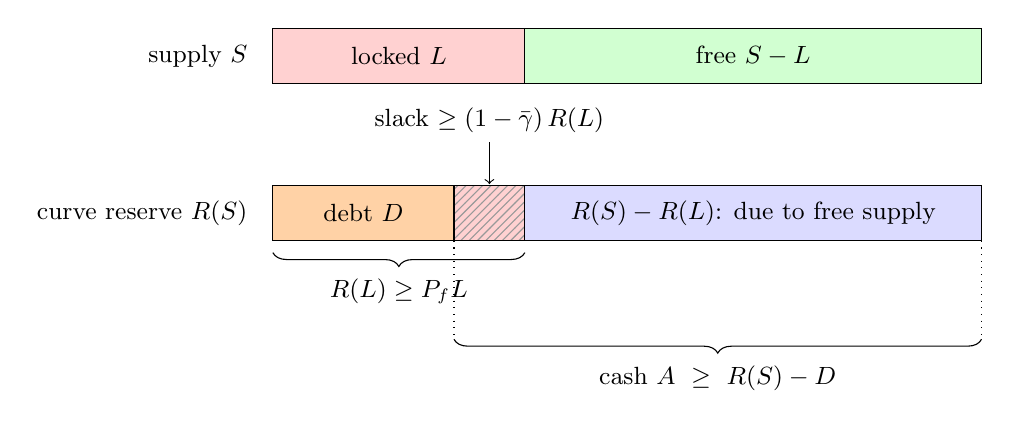
\begin{tikzpicture}[x=1cm,y=1cm,font=\small]
\node[anchor=east] at (-0.2,2.35) {supply $S$};
\draw[fill=red!18] (0,2) rectangle (3.2,2.7); \node at (1.6,2.35) {locked $L$};
\draw[fill=green!18] (3.2,2) rectangle (9,2.7); \node at (6.1,2.35) {free $S-L$};
\node[anchor=east] at (-0.2,0.35) {curve reserve $R(S)$};
\draw[fill=red!18] (0,0) rectangle (3.2,0.7);
\draw[fill=orange!35] (0,0) rectangle (2.3,0.7); \node at (1.15,0.35) {debt $D$};
\draw[pattern=north east lines,pattern color=black!40] (2.3,0) rectangle (3.2,0.7);
\draw[fill=blue!14] (3.2,0) rectangle (9,0.7); \node at (6.1,0.35) {$R(S)-R(L)$: due to free supply};
\draw[decorate,decoration={brace,mirror,amplitude=5pt}] (0,-0.15) -- (3.2,-0.15) node[midway,below=6pt] {$R(L)\ge \Pf L$};
\draw[decorate,decoration={brace,mirror,amplitude=5pt}] (2.3,-1.25) -- (9,-1.25) node[midway,below=6pt] {cash $A\ \ge\ R(S)-D$};
\draw[thin,dotted] (2.3,0) -- (2.3,-1.25); \draw[thin,dotted] (9,0) -- (9,-1.25);
\draw[->,thin] (2.75,1.25) node[above,align=center] {slack $\ge(1-\gbar)\,R(L)$} -- (2.75,0.72);
\end{tikzpicture}
\caption{The balance sheet under $\J$. Debt is at most $\gbar\Pf L\le\gbar R(L)$, a fraction of the reserve of the lowest $L$ units of the curve, so the cash that remains covers the curve return of the entire free supply with slack $(1-\gbar)R(L)$.}\label{fig:sheet}
\end{figure}

\begin{theorem}[Safety]\label{thm:safety}
\begin{enumerate}[label=(\alph*)]
\item The empty state ($S=A=0$, no balances, no loans, $0<\gamma\le\gbar$) is valid and satisfies $\J$, and every operation whose guard holds maps a valid $\J$-state to a valid $\J$-state.
\item In every valid $\J$-state, for every $x$ with $0\le x\le S-L$,
\begin{equation}\label{eq:coverage}
A\ \ge\ \bigl[R(S)-R(S-x)\bigr]+(1-\gbar)\,R(L).
\end{equation}
Hence every \op{Sell} whose guard holds can be paid its full curve return.
\item In every valid $\J$-state, every \op{Borrow} whose guard holds satisfies $b\le A-(1-\gbar)R(S)$, and every \op{Skim} whose guard holds satisfies $w\le A$. Hence both can be paid in full.
\end{enumerate}
\end{theorem}
\begin{proof}
(b) By (J3), (J2) summed over loans, and \cref{lem:R},
\[
A\ \ge\ R(S)-D\ \ge\ R(S)-\gbar\,\Pf L\ \ge\ R(S)-\gbar\,R(L)\ =\ \bigl[R(S)-R(L)\bigr]+(1-\gbar)R(L).
\]
Since $S-x\ge L$ and $R$ is increasing, $R(S)-R(L)\ge R(S)-R(S-x)$.

(c) After a \op{Borrow} whose guard holds, loan $i$ satisfies $d_i\le\gamma\Pf\ell_i\le\gbar\Pf\ell_i$ and the other loans are unchanged, so the new totals satisfy $D+b\le\gbar\Pf L'\le\gbar R(L')\le\gbar R(S)$, where $L'=L+\ell^+\le S$ by (J1). With (J3), $A-b\ge R(S)-(D+b)\ge(1-\gbar)R(S)\ge0$. For \op{Skim}, $w\le A+D-R(S)\le A$ because $D\le\gbar R(S)\le R(S)$.

(a) The empty state is valid and satisfies $\J$ trivially. We check each operation, writing primes for the new state. In each case validity is immediate from the guard and from (b) and (c), which show $A'\ge0$.

\op{Transfer} changes two free balances by opposite amounts and nothing else. \op{Buy}: (J1) is immediate, (J2) is untouched because $p$ and the loans are unchanged, and $A'+D\ge A+D+R(S+x)-R(S)\ge R(S+x)$.

\op{Sell}: (J1) holds by the guard $x\le h_u$. $A'+D=A-o+D\ge R(S)-[R(S)-R(S-x)]=R(S-x)$.

\op{Borrow}: (J1) holds by the guard $\ell^+\le h_i$. (J2) holds for loan $i$ by \eqref{eq:ltv} and $\gamma\le\gbar$. $A$ falls by at most $b$ and $D$ rises by exactly $b$, so $A'+D'\ge A+D$.

\op{Repay}: $A'+D'=A+D$, and (J1) holds because released tokens move from the lock to the free balance. If $r=d_i$ the record is deleted. Otherwise $d_i'=d_i-r>0$ and $\ell_i'=\ell_i-u\ge \ell_i(1-r/d_i)=\ell_i\,d_i'/d_i>0$, so $d_i'\le (d_i/\ell_i)\,\ell_i'\le\gbar\Pf\ell_i'$.

\op{SetLTV}: only $\gamma$ changes, and it stays in $(0,\gbar]$.

\op{Reshape}: (J1) is untouched. (J2) is preserved because debts and locks are unchanged and $\Pf'\ge\Pf$ by (G1). (J3) is (G2).

\op{Skim}: $A'+D=A+D-w\ge R(S)$ by the guard.
\end{proof}

Two remarks on the scope of the theorem. First, the proof uses the schedule only through $R(0)=0$ and the bound $R(b)-R(a)\ge\Pf\,(b-a)$ of \cref{lem:R}, that is, through $p\ge\Pf$. Monotonicity of $p$ is not needed for safety, and the formal statement in \cref{app:lean} assumes only that bound. Monotonicity is what makes $\Pf=p(0)$ the lowest price and $R$ convex, and it is used from \cref{sec:tight} on. Second, the operation set is closed in the following sense: the state changes only through the operations listed above, each of which is covered by part~(a), and an implementation is an instance of the model only if it has no other way to change the state (\cref{sec:conformance}, C7). An implementation may also change the representation of the schedule inside an operation, as the reference model does when a sale retires unminted capacity at the floor (\cref{sec:integer}). Such a change leaves $p$ unchanged on $[0,S)$ and is a \op{Reshape} with $c=0$ that satisfies (G1) and (G2) with equality in $R$, so it is covered.

The proof uses no property of the fee policy, no assumption that any loan is ever repaid, and no property of the schedule beyond monotonicity. The following consequences are stated for \emph{gross} amounts, that is curve returns before any sell fee; \cref{sec:net} treats net amounts.

\begin{corollary}[Redemption at the curve price]\label{cor:redeem}
From any reachable state, any sequence of \op{Sell} operations by holders of free tokens can be executed, each with its full curve return available. The curve return of $x$ tokens is $R(S)-R(S-x)\ge\Pf x$.
\end{corollary}

\begin{corollary}[Exit order]\label{cor:run}
Let free holders redeem $x_1,\dots,x_n>0$ tokens in this order with no other operation in between, and let $x=\sum_k x_k\le S-L$. The curve returns sum to $R(S)-R(S-x)$, independently of the order and of how $x$ is split. The curve return per token is non-increasing in the order of redemption, is at least $\Pf$ for every redeemer, and differs between any two redeemers by at most $p(S^-)-\Pf$.
\end{corollary}
\begin{proof}
The $k$-th redeemer's curve return is $R(S_k)-R(S_k-x_k)$ with $S_k=S-\sum_{j<k}x_j$; the sum telescopes. Monotonicity and the bounds follow from \cref{lem:R}.
\end{proof}

The comparison with the demand-deposit model of \citet{diamond1983} is an analogy, but an instructive one. There, a depositor who arrives after the liquid asset is exhausted receives nothing, and this is what makes a run self-fulfilling. Here the last free token has a curve return of at least $\Pf$ whatever the others do, so a belief that others will redeem cannot make redemption at the floor fail. A first-mover advantage remains for the part of the price above the floor: early redeemers are paid from higher parts of the curve. It is bounded by the premium $p(S^-)-\Pf$ and is a property of every bonding curve, with or without credit.

\begin{corollary}[Non-rivalrous credit]\label{cor:nonrival}
Whether a borrower can borrow $b$ depends only on that borrower's own position and on $(\gamma,\Pf)$, through \eqref{eq:ltv}. It does not depend on other loans, on utilization, or on $A$.
\end{corollary}

\begin{definition}[Liquidation-free]\label{def:liqfree}
A credit facility is \emph{liquidation-free} if (i) no operation other than the borrower's own repayment releases or removes a loan's locked tokens, and (ii) every payment the issuer owes under its operations can be made on every path, including paths on which no loan is ever repaid.
\end{definition}

\begin{corollary}\label{cor:liqfree}
The mechanism of this section is liquidation-free. In every reachable state a borrower recovers all $\ell_i$ locked tokens by paying $d_i\le\gbar\Pf\ell_i$, which is strictly less than their floor value when $\gbar<1$.
\end{corollary}

The price of this property is borne by the borrower who never repays: the tokens stay locked for ever, and the borrower forgoes their residual value. \Cref{sec:incentives} examines when that is a rational choice.

\begin{remark}[The case $\gbar=1$]\label{rem:gbar1}
\Cref{thm:safety} includes $\gbar=1$: coverage then holds with zero slack. A cap strictly below one is needed for three further things: a positive margin against any rounding that is not conservative (\cref{sec:integer}), a positive residual value for every borrower, and the incentive results of \cref{sec:incentives} in their basic form (\cref{sec:general} treats $\gbar=1$).
\end{remark}

\begin{remark}[Floor monotonicity]\label{rem:mono}
The floor price changes only through \op{Reshape}, so by (G1) it never falls. In this model that is a guard, not a theorem. Removing the guard admits unsafe reshapes (\cref{ex:reconf}). The guard is not the weakest condition that preserves $\J$: a funded reshape that lowers the floor while keeping $d_i\le\gbar\Pf'\ell_i$ for every loan would also do so. (G1) is the form of that condition that does not depend on the loan book.
\end{remark}

\begin{remark}[Policy LTV and persistent safety]\label{rem:gamma}
(J2) is stated with the constant cap $\gbar$, not with the current policy $\gamma$. A loan originated at $\gamma=0.9$ still satisfies (J2) after the policy is lowered to $0.8$, but it no longer satisfies $d_i\le\gamma\Pf\ell_i$. The persistent inequality is the one with $\gbar$. \Citet{dabc2026} state the loan bound with the current $\gamma$; when $\gamma$ can be lowered, the form with $\gbar$ is the one that persists.
\end{remark}

\subsection{Tightness of the floor anchor}\label{sec:tight}

\begin{lemma}[Exact coverage condition]\label{lem:exact}
In a valid state with (J1) and no surplus, $A+D=R(S)$, the curve return of the whole free supply can be paid if and only if $D\le R(L)$.
\end{lemma}
\begin{proof}
The curve return of the free supply is $R(S)-R(L)$, and $A=R(S)-D$.
\end{proof}

So what coverage requires is an \emph{aggregate} bound: total debt must not exceed the reserve of the lowest $L$ units of the curve. Rule (J2) enforces it loan by loan through $\Pf\ell_i$, a quantity that depends on nothing but the loan itself. No larger uniform per-token cap works.

\begin{proposition}[Tightness]\label{prop:tight}
Fix any schedule and any number $\lambda>\Pf$. Replace the guard \eqref{eq:ltv} by $d_i+b\le\lambda\,(\ell_i+\ell^+)$. Then there is a reachable state, satisfying (J1) and (J3), in which the curve return of a free holder's \op{Sell} exceeds the cash $A$.
\end{proposition}
\begin{proof}
Charge no fees. By \cref{lem:R} there is an $\ell>0$ with $R(\ell)<\lambda\ell$; choose it small enough that $\ell+y\le C$ for $y=(\lambda/\Pf-1)\,\ell$. From the empty state let account~1 buy $\ell$ tokens and then account~2 buy $y$ tokens, each at the curve cost. Then $A=R(\ell+y)\ge\Pf(\ell+y)=\lambda\ell$. Account~1 locks $\ell$ and borrows $\lambda\ell$, which is available. Now $A=R(\ell+y)-\lambda\ell<R(\ell+y)-R(\ell)$, which is the curve return of account~2's $y$ tokens.
\end{proof}

A cap at the spot price, $\lambda=\gamma\,p(S)$, is the case of an oracle-free loan valued ``at market''; it fails as soon as $\gamma\,p(S)>\Pf$.\footnote{With $\Pf=1$, a spot price of $2$ and $\gamma=0.9$, one borrower locks $100$ floor-priced tokens and borrows $180$; cash is $120$ against a curve return of $200$ for the free supply. Script block N08.}

\begin{remark}[Rules that are not uniform]
The proposition concerns caps that are a fixed amount per locked token. One could instead admit loans as long as $D\le R(L)$, which lends against the premium when $L>S_0$. That rule is rivalrous, since one loan consumes capacity that another could have used, and it is not closed under repayment: when borrower $j$ repays $d_j$ and unlocks $\ell_j$, the bound falls by $R(L)-R(L-\ell_j)$, which can exceed $d_j$, so the remaining loans can violate the rule through no action of their own.
\end{remark}

\subsection{Raising the floor}\label{sec:raise}

\begin{definition}[Lift]
For a schedule $p$, supply $S>0$ and level $y\ge\Pf$, the \emph{lift cost} is
\[
K(y)=\int_0^S\pos{y-p(u)}\,du .
\]
\end{definition}

$K(y)$ is the reserve needed to raise every minted unit priced below $y$ up to $y$. It is continuous and convex with $K(\Pf)=0$, and its one-sided derivatives are the amounts of minted supply priced strictly below, and at or below, the level:
\[
K'_-(y)=\bigl|\{u<S:\,p(u)<y\}\bigr|,\qquad K'_+(y)=\bigl|\{u<S:\,p(u)\le y\}\bigr| .
\]
Because $p$ is right-continuous at $0$, the set $\{u<S: p(u)<y\}$ has positive measure for every $y>\Pf$, so $K$ is strictly increasing on $[\Pf,\infty)$, and it is unbounded. Hence for every budget $c>0$ there is exactly one level $y^\ast>\Pf$ with $K(y^\ast)=c$.

\begin{proposition}[Floor raise by water-filling]\label{prop:raise}
Let a valid $\J$-state have $S>0$ and surplus $W$, and let $0<c\le W$. Let $y^\ast$ be the level with $K(y^\ast)=c$, and let $p'$ be any schedule of capacity at least $S$ with $p'(u)=\max\{p(u),y^\ast\}$ for $u<S$. Then \op{Reshape}$(p',0)$ satisfies (G1) and (G2), the new floor is $y^\ast$, and the surplus falls by exactly $c$.
\end{proposition}
\begin{proof}
$p'(0)=y^\ast\ge\Pf$ gives (G1). $R_{p'}(S)=R_p(S)+K(y^\ast)=R_p(S)+c\le R_p(S)+W=A+D$ gives (G2).
\end{proof}

\begin{figure}[t]
\centering
\begin{tikzpicture}
\begin{axis}[width=0.78\textwidth,height=5.6cm,xlabel={supply},ylabel={price},
  xmin=0,xmax=12000,ymin=0,ymax=2.9,legend pos=north west,legend cell align=left,
  scaled x ticks=false,xtick={0,4000,5000,7500,12000},xticklabels={0,4000,5000,$S{=}7500$,12000},
  tick label style={font=\footnotesize},label style={font=\small},legend style={font=\footnotesize}]
\addplot[const plot,thick,black!55,dashed] table[x=s,y=p] {figures/curve_before.dat};
\addlegendentry{before}
\addplot[const plot,very thick,blue!70!black] table[x=s,y=p] {figures/curve_after.dat};
\addlegendentry{after raise}
\draw[thin,dotted] (axis cs:7500,0) -- (axis cs:7500,2.9);
\fill[blue!25,opacity=0.5] (axis cs:0,1) rectangle (axis cs:4000,1.34);
\fill[blue!25,opacity=0.5] (axis cs:4000,1.2) rectangle (axis cs:5000,1.34);
\node[font=\footnotesize,anchor=west] at (axis cs:300,1.55) {$c=1500$ fills to $y^\ast=1.34$};
\end{axis}
\end{tikzpicture}
\caption{A floor raise is water-filling of the minted part of the curve. Floor $1.00$ on $4000$ tokens, steps of $1000$ tokens at $1.2,1.4,\dots$, supply $7500$. A budget of $1500$ lifts the floor to $1.34$: $800$ to reach $1.2$ over $4000$ tokens, then $700$ over $5000$ tokens. Script block N10.}\label{fig:raise}
\end{figure}

For a stepped curve, $y^\ast$ is found by absorbing steps from the bottom until the budget is exhausted, which is the step-absorption algorithm of \vone; \cref{fig:raise} shows an example. The two ``modes'' of that algorithm are the two regimes of the slope of $K$: below the marginal price $p(S^-)$ the level rises against the minted supply underneath it, and above $p(S^-)$ it rises against the whole supply $S$. The proposition leaves the unminted part of the schedule free. Retiring unminted capacity priced at or below the new floor, as the earlier paper does, means that immediately after the raise no token can be minted at the floor price. A later redemption can make minting at the current floor possible again. In the reference model this occurs when a redemption reopens capacity on the last remaining step of a curve, which is never retired, or when a full redemption removes the exhausted floor step and exposes the next step as the new floor.

Three properties of the lift cost drive the economics. First, the cost of a marginal raise is the minted supply at or below the level, \emph{including locked tokens}: loans that stay open make every later raise more expensive. Second, redemptions at the floor reduce that supply, so a contraction makes later raises cheaper per unit of budget. Third, a raise increases every borrower's limit \eqref{eq:ltv} by $\gamma\,(y^\ast-\Pf)\,\ell_i$ without any action by the borrower, while the debt is unchanged.

\subsection{Reconfiguration: safety is not fairness}\label{sec:reconf}

By \cref{thm:safety}, the guards (G1) and (G2) are sufficient for the safety of any change to the curve. Dropping either one admits unsafe changes; for (G2) this is obvious, and for (G1) an example follows.

\begin{example}[A reshape without the floor guard]\label{ex:reconf}
Take two one-token steps priced $10$ and $30$, so $R(2)=40$, no fees, and $\gamma=\gbar=0.9$. One token is locked against a debt of $9$; cash is $31$. Reconfigure the prices to $8$ and $32$. The reserve is unchanged, $R'(2)=40$, and no price falls by more than $2$, so reserve equality, a bounded price loss and a cumulative budget, the conditions listed in Definition~3.5 of \vone, can all hold. But the floor is now $8<9$, so the loan exceeds the floor value of its collateral, and the free token's curve return is $32$ against cash of $31$. With (G1), which the earlier paper assumes as a precondition, the reconfiguration is rejected. Script block N06.
\end{example}

Safety says nothing about who gains and who loses. Tokens are fungible and are not attached to positions on the curve, so the natural object is the payoff of a set of holders who exit together.

\begin{definition}[Exit payoff]
In a state with supply $S$ and locked supply $L$, the \emph{exit payoff} of a coalition of free holders that redeems $x\le S-L$ tokens is its curve return $G(x)=R(S)-R(S-x)$.
\end{definition}

A reshape $p\to p'$ at fixed supply changes the exit payoff of the coalition of size $x$ by
\[
G'(x)-G(x)=\bigl[R_{p'}(S)-R_p(S)\bigr]-\bigl[R_{p'}(S-x)-R_p(S-x)\bigr].
\]
Call a reshape \emph{reserve-neutral} if $R_{p'}(S)=R_p(S)$: it uses no surplus and no new funding. A reserve-neutral reshape harms some currently feasible exit if and only if $R_{p'}(z)>R_p(z)$ for some depth $z\in[L,S]$, and we define its \emph{exit distortion} as
\[
\Delta(p,p')=\max_{z\in[L,S]}\pos{R_{p'}(z)-R_p(z)},
\]
the largest loss of curve return, in reserve units, that it imposes on any coalition that could exit now. $\Delta$ measures gross, immediate exit opportunities; it does not capture changes in fees, in future opportunities, or in borrowing capacity. Moving reserve value \emph{down} the curve, toward the floor, increases $R_{p'}(z)$ at small depths. A reserve-neutral reshape that raises the floor always does this near depth zero, so when no tokens are locked it lowers the exit payoff of every sufficiently large coalition short of the whole supply; the coalition of all holders receives $R(S)$ before and after.

\begin{proposition}[Harvesting the premium under locked supply]\label{prop:harvest}
In a valid $\J$-state with $L>0$, let $p'$ be a schedule that agrees with $p$ on $[L,C)$ and satisfies $p'(0)\ge p(0)$ and $R_{p'}(L)=R_p(L)$. Then \op{Reshape}$(p',0)$ is admissible, reserve-neutral, and has zero exit distortion. The flat schedule $p'\equiv R_p(L)/L$ on $[0,L)$ is of this kind; it raises the floor to $R_p(L)/L$, which is strictly above $\Pf$ whenever $L>S_0$. For this flat schedule $R_{p'}(z)\ge R_p(z)$ for all $z\le L$, with equality at $z=0$ and $z=L$ and strict inequality for $0<z<L$ when $L>S_0$. Hence, once loans have been repaid, a coalition whose exit reaches a depth strictly between $0$ and $L$ has a lower exit payoff than before.
\end{proposition}
\begin{proof}
$R_{p'}=R_p$ on $[L,S]$ because the schedules agree above $L$ and $R_{p'}(L)=R_p(L)$; hence (G2) holds and $\Delta=0$, and (G1) holds by assumption. If $L<C$, the flat schedule is non-decreasing across $L$ because the average of $p$ over $[0,L)$ is at most $p(L)$; if $L=C$ there is no price above $L$ and nothing to check. The flat level exceeds $\Pf$ when $p$ is not constant on $[0,L)$. For $z\le L$, $R_{p'}(z)=\tfrac zL R_p(L)\ge R_p(z)$ by \cref{lem:R}; equality at an interior point would force the convex function $R_p$ to be linear on $[0,L]$.
\end{proof}

\Citet{dabc2026} call this operation ``idle premium harvesting'': it frees capital that sits idle behind locked tokens. \Cref{prop:harvest} gives the precise sense in which it is harmless, namely for every exit that is feasible while the tokens stay locked, and the precise sense in which it is not: it lowers the payoff of deep partial exits after repayment in favor of those who exit last, and it raises every borrower's limit.

Two practical points follow. A bound on dilution should be stated on $\Delta$ relative to $R(S)$, which has units of value, and not on pointwise price changes in absolute units, which lose meaning as the price scale changes. And a cumulative budget that the reconfiguring authority can itself reset bounds the harm between resets only; it protects holders only if the reset is immutable, or delayed long enough for holders to exit first.

\subsection{Gross floor and net floor}\label{sec:net}

\Cref{cor:redeem,cor:run} concern curve returns. If redemption carries a proportional fee $f_s$, the holder receives $(1-f_s)\,[R(S)-R(S-x)]$.

\begin{proposition}[Net floor]\label{prop:net}
If the sell fee charged on every redemption, in every state and for every size, is at most a constant $\fsbar<1$, then every redemption pays at least $(1-\fsbar)\,\Pf$ per token, and this bound never falls. Without such a cap the net redemption value of a token need not be monotone, although $\Pf$ is.
\end{proposition}

We call $(1-\fsbar)\Pf$ the \emph{net floor}. The distinction matters in practice. The fee policy studied in \vone{} is highest at the floor: with their reported parameters the sell-side multiplier at the floor is $2.5$, and the combined multiplier is capped at $15$ times the base fee. Under such a policy the statement ``every token can be redeemed at or above the floor'' holds for the curve return only. All loan statements in this paper are gross as well: (J2) says that the debt is below the gross floor value of the lock.

\subsection{Integer arithmetic}\label{sec:integer}

Contracts compute with integers. \Cref{thm:safety} survives if every rounding goes against the party that receives value.

\begin{proposition}[Integer refinement]\label{prop:int}
Let token and reserve amounts be integers and let $R$ be evaluated exactly as a rational number. Suppose that (r1) a buyer pays at least $R(S+x)-R(S)$; (r2) in a sale the cash $A$ falls by at most $R(S)-R(S-x)$, counting the seller's proceeds and any part of the fee that leaves the mechanism in the same operation; (r3) the guard \eqref{eq:ltv} is evaluated as an exact inequality between integers, equivalently the lock required for a requested debt is rounded \emph{up}; (r4) a full repayment releases the whole lock and a partial repayment releases $\lfloor\ell_i r/d_i\rfloor$ or less; and (r5) the guards (G1) and (G2) are evaluated exactly. Then \cref{thm:safety} holds as stated.
\end{proposition}
\begin{proof}
Each of (r1)--(r5) implies the real-valued guard or effect used in the proof of \cref{thm:safety}.
\end{proof}

The corollaries on amounts then hold up to rounding, under one further condition. Rule (r2) is an upper bound and by itself guarantees no minimum. If the curve return is computed with exactly one rounding, as $\lfloor R(S)-R(S-x)\rfloor$, then a redemption of $x$ token units has an integer curve return of at least $\lfloor\Pf x\rfloor$, and the sum of the returns of a split redemption can fall short of the unsplit return by less than one reserve unit per part.

Rule (r3) is the one that is easy to get wrong. If the lock for a requested debt $d$ is computed as $\lfloor d/(\gamma\Pf)\rfloor$, the borrower's limit is exceeded whenever the division is inexact, and a small enough request locks nothing at all. With a floor price of $2$, an LTV of $90\%$ and a request of $3$, the rounded-down lock is $1$ token of floor value $2$: the debt exceeds not only the LTV limit but the floor value itself. With a floor price of $100$, a request of $1$ locks $0$ tokens (script block N07). The excess per borrowing call is less than $\gamma$ times the value of one token unit. Whether that is negligible depends on the token's unit size and on how many calls can be made; in any case (J2) is then false as stated, and the margin $1-\gbar$ is all that stands between the accumulated error and the floor value.

Net amounts need the same care. If the net proceeds of a redemption are computed with one rounding, as $\lfloor(1-f_s)\,[R(S)-R(S-x)]\rfloor$, then a redemption of $x$ token units pays at least $\lfloor(1-\fsbar)\Pf x\rfloor$. Rounding the curve return down and then the fee up can lose a further unit, which matters for \cref{prop:netclose}.

An implementation must also define its floor when the lowest step is exhausted. The reference model of \cref{sec:evidence} keeps $\Pf=p(0)$ and a positive capacity: when a sale takes the supply below the floor capacity, that capacity is reduced to the supply, and if it reaches zero the step is dropped and the next step becomes the floor; the last remaining step of a curve is never reduced.

\subsection{Carrying cost}\label{sec:carry}

A perpetual loan with a one-time fee has no carrying cost, and \cref{sec:incentives} shows what that does to incentives. \Citet{dabc2026} obtain liquidation-free credit by excluding interest. A weaker condition suffices.

\begin{proposition}[Capped accrual]\label{prop:carry}
Add an operation \op{Accrue}$(i,\delta)$ with guard $\delta>0$, $d_i+\delta\le\gbar\Pf\ell_i$, and effect $d_i\gets d_i+\delta$. Then \cref{thm:safety} still holds.
\end{proposition}
\begin{proof}
(J2) is the guard. $A+D$ increases, so (J3) is preserved. Parts (b) and (c) use only $\J$ and validity.
\end{proof}

Interest is therefore compatible with liquidation-free credit as long as it stops at the cap. A loan originated at $\gamma<\gbar$ can accrue until its debt has grown by the factor $\gbar/\gamma$, and every floor raise restores headroom. What is incompatible is \emph{uncapped} accrual: debt growing at a rate for ever stays below $\gbar\Pf(t)\ell$ only if the floor grows at least as fast, which no fee flow guarantees.

The accounting of accrual is easy to misread. \op{Accrue} increases the surplus $W$ without any reserve being paid in. What has increased is the borrower's repayment obligation; the borrower's residual value $\Pf\ell_i-d_i$ has fallen by the same amount. Under $\J$ that additional claim releases backing capacity: it can fund a floor raise, or a \op{Skim} that withdraws cash already held. Neither endangers coverage, because $D\le\gbar\Pf L$ still holds and locked tokens cannot be redeemed; in particular $A\ge(1-\gbar)R(S)$ throughout. Economically, capped accrual transfers value from the borrower's residual to the other holders or to the recipient of the skim, up to the fraction $\gbar$ of the lock's floor value, without ever touching the locked tokens. Whether to adopt it is a design choice; the point here is that safety does not forbid it.

\section{Credit Capacity and Collateral Release}\label{sec:credit}

\Cref{lem:exact} gives the cash needed for redemptions at one state. A lending rule must also cover the states that borrowers can create by repaying. This section characterizes that requirement for a fixed curve. It then gives two ways of lending beyond the floor: commit an additional reserve, or change the collateral released by a repayment. The additional credit has a cost in each case. The first uses capital that cannot be skimmed; the second restricts withdrawal and splitting of positions. These are extensions of the model, not claims that its original floor bound is incorrect.

\subsection{Repayment rights and cash coverage}\label{cr:rights}

Fix a schedule $p$ and its reserve function $R$. There are finitely many loans $(\ell_i,d_i)$, with $\ell_i,d_i>0$, total lock $L\le S$, and cash $A\ge0$. Custody holds, and $W=A+D-R(S)\ge0$. We allow debts above the floor, so (J2) is \emph{not} assumed. Initially consider only repayments and redemptions at their full gross curve return. There is no new borrowing, minting, reshaping, accrual, reserve withdrawal or fee retention. Thus $W$ is constant. Borrowers may supply the cash needed to repay; safety is required for all allowed repayment choices, whether or not those choices maximize their payoffs.

For each loan, let $\mathcal E_i\subseteq[0,\ell_i]\times[0,d_i]$ be the closure of the set of residual pairs $(q_i,b_i)$, locked tokens and remaining debt, attainable by a finite sequence of repayments. It includes the initial pair and $(0,0)$. Repayment rights are local to the loan: they do not depend on other loans, free balances or redemptions. Each combination of attainable pairs can therefore be reached by making the loans' repayments in turn, before any redemption. Taking the closure includes limits of such combinations; the cash inequalities below are continuous and are unchanged by this convention. Full repayment releases the whole lock. We call a state \emph{safe under its repayment rights} if every finite sequence of these repayments and gross redemptions can be executed without a cash shortfall.

\begin{theorem}[Coverage under repayment rights]\label{cr:kernel}
The state is safe under its repayment rights if and only if
\begin{equation}\label{cr:allpairs}
\sum_i b_i\;\le\;W+R\!\left(\sum_i q_i\right)
\qquad\text{for every }(q_i,b_i)\in\mathcal E_i\text{ for all }i.
\end{equation}
When $W=0$, this is equivalent to the separate conditions
\begin{equation}\label{cr:individual}
b\le R(q)\qquad\text{for every }(q,b)\in\mathcal E_i\text{ and every }i.
\end{equation}
\end{theorem}
\begin{proof}
After any repayments and redemptions, write $S',D',L',A'$ for the current state. Repayments preserve $A+D$, and a gross redemption reduces $A$ and $R(S)$ by the same amount. Thus $A'+D'-R(S')=W$. Redeeming all free tokens would leave cash
\[
A'-[R(S')-R(L')]=W+R(L')-D'.
\]
If \eqref{cr:allpairs} holds, that cash is non-negative at every possible loan state; every smaller redemption can also be paid. Repayments add cash. Conversely, a violation at an attainable residual configuration is exposed by making those repayments and then redeeming all free tokens. A strict violation at a limit configuration is also a violation at a nearby attainable one.

For the last claim, convexity and $R(0)=0$ give
\begin{equation}\label{cr:superadd}
\sum_i R(q_i)\le R\!\left(\sum_iq_i\right).
\end{equation}
Indeed $R(q_i)\le q_i R(Q)/Q$ for $Q=\sum_iq_i>0$. Hence \eqref{cr:individual} suffices. It is necessary because all loans other than $i$ can be fully repaid, leaving their residual pairs equal to $(0,0)$.
\end{proof}

For any repayment rights we write $W_{\min}$ for the least reserve that satisfies \eqref{cr:allpairs}: the supremum of $\sum_ib_i-R(\sum_iq_i)$ over attainable configurations, which is at least zero. \Cref{cr:buffer} computes it for proportional release.

The quantifier over future repayments is essential. For $R(q)=q+q^2/2$, a one-token lock against debt $3/2$ satisfies the current condition $D=R(L)$. If $S=L=1$ and $W=0$, cash is zero. Repaying $3/4$ and releasing half the collateral makes $3/4$ cash available, but redeeming the released half costs $R(1)-R(1/2)=7/8$. The shortfall is $1/8$. No price movement or other borrower is needed.

\subsection{Proportional release and the committed reserve}\label{cr:proportional}\label{sec:credit-buffer}

Under proportional release, $\mathcal E_i=\{(x\ell_i,xd_i):0\le x\le1\}$. Put $a_i=d_i/\ell_i$. For $0\le q\le L$, define
\begin{equation}\label{cr:envelope}
H(q)=\max\left\{\sum_i a_iq_i:
0\le q_i\le\ell_i,\ \sum_iq_i=q\right\}.
\end{equation}
This is the fractional-knapsack envelope: retain collateral from loans with the largest $a_i$ first \citep{kellerer2004}. It is continuous, concave and piecewise linear. For $L>0$, if $Z$ takes value $a_i$ with probability $\ell_i/L$, then $H(q)=L\int_{1-q/L}^{1}F_Z^{-1}(u)\,du$, an upper integrated-quantile function \citep{gushchin2017}. For an empty book, set $H(0)=W_{\min}=0$. The sorting argument is classical; its role here is to identify the residual loan book that places the greatest demand on cash.

\begin{theorem}[Exact buffer for proportional release]\label{cr:buffer}
With proportional release, the least non-negative committed reserve required by \cref{cr:kernel} is
\begin{equation}\label{cr:wmin}
W_{\min}=\max_{0\le q\le L}\{H(q)-R(q)\}.
\end{equation}
In particular, when $W=0$, safety under all repayment choices holds if and only if $d_i\le\Pf\ell_i$ for every loan. This necessity applies to heterogeneous and state-dependent loan allocations, not only to a uniform cap.
\end{theorem}
\begin{proof}
At fixed residual total $q$, \eqref{cr:envelope} is the largest possible remaining debt. Substitution in \cref{cr:kernel} gives \eqref{cr:wmin}; its maximum is at least zero because $H(0)=R(0)=0$. For $W=0$, \eqref{cr:individual} requires $xd_i\le R(x\ell_i)$ for every $x>0$. Divide by $x\ell_i$ and let $x$ decrease to zero to obtain $a_i\le\Pf$. Conversely, $a_iq_i\le\Pf q_i\le R(q_i)$, so \eqref{cr:individual} holds.
\end{proof}

For a uniform cap per token, the necessity of the floor bound is \cref{prop:tight}. The statement here extends it in two ways: it holds loan by loan for any allocation of debt, and it follows from the repayment rights alone, without constructing a sequence of borrowing operations.

The function $H-R$ is concave. Its maximum is found where the non-increasing slope of $H$ crosses the non-decreasing price $p$, including endpoints and jumps. Sorting the ratios takes $O(n\log n)$ comparisons. With rational stepped or piecewise-affine prices, a scan of the price and collateral breakpoints finds the maximum exactly. \Cref{cr:algorithm} gives the representation and algorithm; an arbitrary price function instead requires an evaluation or optimization oracle.

\paragraph{Keeping the reserve committed.}
For this extended design, $W$ is not all available for withdrawal. The safe skim guard is $w\le W-W_{\min}$. A repayment restricts the remaining possible residual configurations, so it cannot increase $W_{\min}$ at a fixed curve. Gross sales leave both $W$ and the loan book unchanged; retaining fees can only increase $W$. New lending may be admitted by checking $W'\ge W_{\min}'$ in the resulting state. That test also implies $A'\ge0$, since the initial residual configuration gives $D'\le W'+R(L')\le W'+R(S')$. A reshape needs the same test with the new reserve function and the repayment rights that will remain in force. These are guards for a different mechanism; the original \op{Skim} guard in \cref{sec:model} must not be used with above-floor proportional loans. Full derivations are in \cref{cr:guards}.

\subsection{Allocation of a fixed reserve}\label{cr:allocation}

\begin{proposition}[Equal ratios and aggregate capacity]\label{cr:capacity}
Fix positive lock sizes with total $L>0$. Among allocations with total debt $D$, assigning $d_i=(D/L)\ell_i$ minimizes $W_{\min}$, weakly. The greatest aggregate debt consistent with proportional release and a committed reserve $W\ge0$ is
\begin{equation}\label{cr:dmax}
D_{\max}=L\inf_{0<q\le L}\frac{R(q)+W}{q}.
\end{equation}
An allocation with equal ratios attains this bound.
\end{proposition}
\begin{proof}
Concavity, $H(0)=0$ and $H(L)=D$ imply $H(q)\ge Dq/L$. Equal ratios attain equality at every $q$, so they weakly minimize \eqref{cr:wmin}. For that allocation, the safety constraints are $(D/L)q\le R(q)+W$ for every $q>0$, which are equivalent to \eqref{cr:dmax}. The infimum is finite and the corresponding constant ratio satisfies every constraint, whether or not the infimum is attained at a positive $q$.
\end{proof}

The minimizer need not be unique. This is a chord comparison for the classical envelope, rather than a new general optimization method. Its implication for credit is that two books with identical supply and total debt can require different reserves. With $R(q)=q+q^2/2$, $L=1$ and $D=3/2$, an equal ratio of $3/2$ requires $W_{\min}=1/8$. Two locks of $1/2$ with debts $1$ and $1/2$ require $W_{\min}=3/8$: the highest ratio is retained while the other loan is repaid. The reserve requirement triples although aggregate utilization is unchanged.

\begin{figure}[t]
\centering
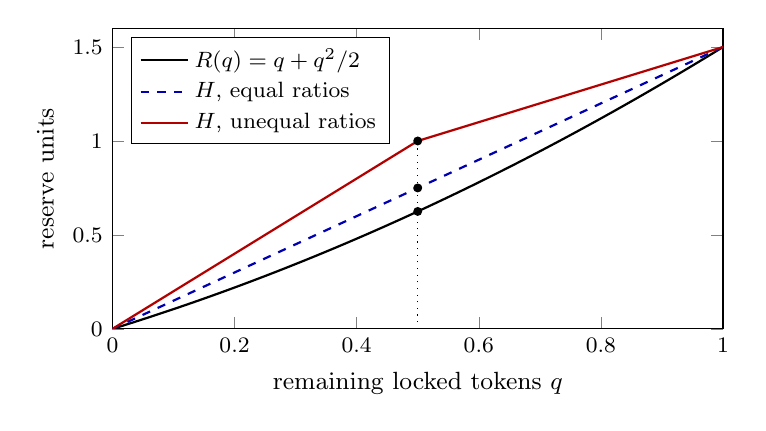
\begin{tikzpicture}
\begin{axis}[width=0.77\textwidth,height=5.4cm,
  xlabel={remaining locked tokens $q$},ylabel={reserve units},
  xmin=0,xmax=1,ymin=0,ymax=1.6,
  legend pos=north west,legend cell align=left,
  tick label style={font=\footnotesize},label style={font=\small},
  legend style={font=\footnotesize}]
\addplot[thick,black,domain=0:1,samples=101] {x+x*x/2};
\addlegendentry{$R(q)=q+q^2/2$}
\addplot[thick,dashed,blue!70!black,domain=0:1,samples=2] {1.5*x};
\addlegendentry{$H$, equal ratios}
\addplot[thick,red!70!black] coordinates {(0,0) (0.5,1) (1,1.5)};
\addlegendentry{$H$, unequal ratios}
\draw[thin,dotted] (axis cs:0.5,0) -- (axis cs:0.5,1);
\addplot[only marks,mark=*,mark size=1.4pt,black]
  coordinates {(0.5,0.625) (0.5,0.75) (0.5,1)};
\end{axis}
\end{tikzpicture}
\caption{The required reserve is the greatest vertical distance from $R$ to the debt envelope $H$. Both books have $L=1$ and $D=3/2$. Their maximum gaps occur at $q=1/2$ and are $1/8$ for equal ratios and $3/8$ for the two unequal ratios. These quantities are checked in script block CF01.}\label{cr:figure}
\end{figure}

For the linear price $p(q)=P+kq$, with $P>0$ and $k>0$, minimizing \eqref{cr:dmax} gives
\begin{equation}\label{cr:linearcapacity}
\frac{D_{\max}}L=
\begin{cases}
P, & W=0,\\[2pt]
P+\sqrt{2kW}, & 0<W\le kL^2/2,\\[2pt]
P+kL/2+W/L, & W>kL^2/2.
\end{cases}
\end{equation}
The interior minimizing depth is $\sqrt{2W/k}$. The formula describes cash coverage, not a positive residual for every borrower. An above-floor proportional loan can become worth less than its debt after a partial repayment, even when the committed reserve makes every free redemption payable. For example, in the one-token case above, $W=1/8$ pays the released half, but the remaining debt $3/4$ exceeds $R(1/2)=5/8$. A collateral-funded close is a separate requirement.

\paragraph{Cash coverage is not an incentive to repay.}
The buffer makes above-floor loans payable; it does not make them worth repaying, and the incentive results of \cref{sec:incentives} do not carry over. For exit routing, a holder whose tokens would redeem for a gross value $v$ per token receives $(1-f_s)v$ by redeeming and $(1-\phi)a$ by borrowing at the ratio $a$ and never repaying. Abandonment pays whenever $(1-\phi)\,a>(1-f_s)\,v$, the condition of \cref{prop:route} with $\gamma\Pf$ replaced by $a$. For a holder who redeems at the floor, $v=\Pf$, and a ratio $a>\Pf$ satisfies the condition unless the fees are at least as large as the lending premium, $(1-f_s)/(1-\phi)\ge a/\Pf$. The rule $\gbar+\fsbar<1$ guaranteed the opposite inequality at every fee within the cap; lending above the floor removes that guarantee.

Borrowers can do better than choose between repaying in full and abandoning. They can repay in part, redeem the collateral that the repayment releases, and abandon the rest. The next result says exactly how much this takes out.

\begin{proposition}[What a committed reserve can lose]\label{cr:extraction}
In the setting of \cref{cr:rights}, with no fees, let the book be safe under its repayment rights, that is, $W\ge W_{\min}$. Let a coalition hold all $L=S$ tokens, locked against the loans of the book, and let the reserve $W$ have been paid in by someone else.
\begin{enumerate}[label=(\alph*)]
\item If the coalition repays down to an attainable residual configuration with total lock $Q$ and total debt $B$, redeems the released tokens and never repays the rest, it receives $B-R(Q)$ more than by repaying every loan and redeeming every token. The supremum of this gain over attainable configurations, which is the maximum over their closure, is $W_{\min}$, the least reserve that \cref{cr:kernel} requires. Under proportional release the supremum is attained.
\item After a path that attains this maximum the issuer holds cash $W-W_{\min}$.
\item Under proportional release, a book that is admitted with total debt $D_{\max}$ of \eqref{cr:dmax} and $W>0$ has $W_{\min}=W$: the coalition can take the whole reserve.
\item For a coalition that buys the $L$ tokens from an empty curve and pays a buy fee $f_b$, an origination fee $\phi$ and a sell fee $f_s$, all proportional and paid out of the mechanism, the profit of the path in (a) is
\[
\Pi=B-R(Q)-f_b\,R(L)-\phi\,D-f_s\,\bigl[R(L)-R(Q)\bigr].
\]
\item Under the curve-valued contract of \cref{cr:nonlinear} every attainable configuration has $B\le R(Q)$, so the gain in (a) is never positive.
\end{enumerate}
\end{proposition}
\begin{proof}
Because the book is safe under its repayment rights, every repayment and redemption below can be executed; without that hypothesis $B-R(Q)$ is still the difference of the two cash flows as written, but the issuer may run out of cash before the redemption is paid. (a) Repaying down to the configuration costs $D-B$ and the released $L-Q$ tokens redeem for $R(L)-R(Q)$; repaying everything costs $D$ and returns $R(L)$. The difference is $B-R(Q)$. By \cref{cr:kernel} the least admissible reserve is the supremum of $\sum_ib_i-R(\sum_iq_i)$ over attainable configurations, equivalently its maximum over their closure, and it is at least zero because $(0,0)$ is attainable for every loan. (b) The proof of \cref{cr:kernel} gives the cash after the path as $W+R(Q)-B$. (c) Because $W>0$, the function $(R(q)+W)/q$ tends to infinity as $q\downarrow0$ and is continuous on $(0,L]$, so the infimum in \eqref{cr:dmax} is attained at some $q^\ast>0$, where $(D_{\max}/L)\,q^\ast=R(q^\ast)+W$. By concavity $H(q^\ast)\ge D_{\max}q^\ast/L$, so $H(q^\ast)-R(q^\ast)\ge W$, and admission requires $W_{\min}\le W$. (d) The purchase costs $(1+f_b)R(L)$, the loans pay out $(1-\phi)D$, the repayment costs $D-B$ and the redemption returns $(1-f_s)[R(L)-R(Q)]$; the sum is $\Pi$. (e) The persistent condition \eqref{cr:nonlinearcover} holds at every attainable configuration, so $B\le\gbar\sum_iR(q_i)\le R(Q)$ by \eqref{cr:superadd}.
\end{proof}

The reserve that makes a proportional book safe is thus exactly the amount that a coalition of its borrowers can extract from it. Take $R(q)=q+q^2/2$, $L=S=1$ and $W=0.08$, which is below the threshold $kL^2/8=0.125$ at which $D_{\max}$ passes the redemption value $R(L)$ of the whole collateral. Then $D_{\max}=1.4<R(1)=1.5$, so repaying in full is still better than abandoning in full. But buying the token for $1.5$, borrowing $1.4$, repaying $0.84$ to release $0.6$ tokens, redeeming them for $1.02$ and leaving $0.4$ tokens locked against a debt of $0.56$ nets $0.08$: the whole reserve. The issuer is left with no cash and a residual loan of $0.56$ against collateral that redeems for $R(0.4)=0.48$: the loan is under-collateralized, in a state that remains safe under its repayment rights. With all three fees at $1\%$ the profit is $0.0408$ (script block N16). The statement is about a strategy that is available, under the stated assumptions on access and on who funded the reserve; it is not a prediction of what borrowers do, and a borrower who paid in the reserve counts that payment as a cost. The borrower's position is the residual claim of the corporate-debt model, the right to recover the collateral by paying the debt or to walk away \citep{merton1974}, and $W_{\min}$ is capital held against the worst admissible scenario, in the spirit of, though not shown to satisfy the axioms of, a coherent risk measure \citep{artzner1999}.

Two consequences follow. At the maximum admitted credit \eqref{cr:dmax}, the committed reserve is exposed to complete loss under the strategy above: it is first-loss capital for that path, though other repayment paths return it. And the amount that must stay committed is the current $W_{\min}$, not $W$: a repayment narrows the set of residual configurations and can lower the requirement, after which the difference may be withdrawn while the loan is open. In the example, repaying $1.12$ leaves $0.2$ tokens against a debt of $0.28$ and a requirement of $0.06$, so $0.02$ of the reserve is free. A path that repays and abandons can instead use up the cash and leave the remaining requirement committed for good. The curve-valued contract below does not have the defect, by part~(e), and under $\gbar+\fsbar<1$ redeeming a lock pays more than abandoning it.

\subsection{More credit with a different release rule}\label{cr:nonlinear}\label{sec:credit-release}

There is also a way to use the curve premium without an additional committed reserve. Suppose a partial repayment reduces debt but releases no collateral until the loan is fully repaid. By \cref{cr:kernel}, with $W=0$ such a book is safe under all repayments if and only if
\begin{equation}\label{cr:fullrelease}
d_i\le R(\ell_i)\qquad\text{for every loan}.
\end{equation}
Each remaining debt is at most its initial debt at the unchanged lock, and fully repaid loans disappear. Thus \eqref{cr:fullrelease} is the largest per-loan cap compatible with these rights and with the possibility that every other borrower exits.

Partial collateral release is possible if its amount is changed. Consider the operations of \cref{sec:model}, with the following replacements. The persistent loan condition is
\begin{equation}\label{cr:nonlinearcover}
d_i\le\gbar R(\ell_i),\qquad 0<\gbar\le1.
\end{equation}
A borrow is guarded by $d_i+b\le\gamma R(\ell_i+\ell^+)$, with $0<\gamma\le\gbar$. A partial repayment of $r$ may release $u\in[0,\ell_i]$ only if $d_i-r\le\gbar R(\ell_i-u)$; full repayment releases the whole lock. A reshape preserves \eqref{cr:nonlinearcover} for every loan under the new $R$, as well as satisfying (G1) and (G2). Custody, the definitions of $A,D,W$, and the remaining operations are unchanged. The release rule and the debt anchor are both different from those of the original model.

\begin{proposition}[Safety with a curve-valued lock]\label{cr:nonlinearsafety}
These operations preserve custody, \eqref{cr:nonlinearcover} and $A+D\ge R(S)$. Every free-token gross redemption and every admitted loan can be paid in full, without any repayment by another borrower. If proportional sell fees satisfy $f_s\le\fsbar$ and $\gbar+\fsbar\le1$, every loan can also be closed from its own collateral. The close leaves a positive residual when $\gbar+\fsbar<1$.
\end{proposition}
\begin{proof}
By \eqref{cr:superadd}, $D\le\gbar\sum_iR(\ell_i)\le\gbar R(L)$. This is the aggregate bound used in the coverage and cash-payout steps of \cref{thm:safety}. The modified borrow, repayment and reshape guards preserve the new individual condition; the other induction steps are unchanged. In particular a borrow gives $D+b\le\gbar R(S)$, so $A-b\ge(1-\gbar)R(S)$. For a close, monotonicity of $p$ gives
\[
R(S)-R(S-\ell_i)\ge R(\ell_i),
\]
and net proceeds are therefore at least $(1-\fsbar)R(\ell_i)\ge d_i$. Use the atomic netting of \cref{prop:netclose}. If $G=R(S)-R(S-\ell_i)$ is the gross return, the combined reserve outflow is at most $G-d_i$, and
\[
A-(G-d_i)=W+R(S-\ell_i)-(D-d_i)\ge0,
\]
because the other locks total at most $S-\ell_i$ and satisfy \eqref{cr:superadd}. With a strict inequality between the caps, the borrower's residual is at least $(1-\fsbar-\gbar)R(\ell_i)>0$.
\end{proof}

Since $R$ is strictly increasing, the largest release allowed by the new repayment guard is
\begin{equation}\label{cr:maxrelease}
u_{\max}(r)=\ell_i-R^{-1}\!\left(\frac{d_i-r}{\gbar}\right).
\end{equation}
At a loan's limit $d_i=\gbar R(\ell_i)$, convexity implies $u_{\max}(r)\le\ell_i r/d_i$. Paying half the debt therefore need not release half the tokens. In the preceding example with $\gbar=1$, repaying $3/4$ releases $2-\sqrt{5/2}\simeq0.418861$ tokens, whose curve return is exactly $3/4$. An integer implementation must round the remaining required lock upward; this section's result is real-valued, not a verification of such an implementation.

\paragraph{The stronger reshape guard matters.}
Let $p(q)=1+q$, $S=2$, one token locked against $d=3/2$, one token free, and $A=5/2$. Replace the curve by prices $1$ on $[0,1)$ and $3$ on $[1,2)$. The floor remains $1$ and total reserve remains $R(2)=4$, so (G1) and (G2) hold. But the new $R(1)=1$ no longer covers the loan, and the free token's return $3$ exceeds cash. Requiring $d_i\le\gbar R_{p'}(\ell_i)$ rejects this change. A sufficient condition that avoids inspecting each loan is $R_{p'}(z)\ge R_p(z)$ for all $z\le S$, together with funding; water-filling raises satisfy this condition. The new release rule can depend on the curve, so the later repayment-deferral results for a fixed loan-local release rule do not automatically extend to it.

\subsection{Pooling, splitting and independent exit}\label{cr:pooling}

The additional capacity in \eqref{cr:fullrelease} depends on position size. Combining locks $x,y$ increases the maximum debt by
\begin{equation}\label{cr:poolgain}
R(x+y)-R(x)-R(y)
=\int_0^y[p(x+u)-p(u)]\,du\ge0.
\end{equation}
For $p(q)=P+kq$ the gain is $kxy$. This is the value, in lending capacity, of keeping the collateral subject to a joint release condition. A split need not be feasible after the additional credit has been drawn.

\begin{proposition}[Arbitrary independent splitting]\label{cr:splitting}
Suppose $W=0$ and a loan $(\ell,d)$ may be split into $n$ independently repayable loans $(\ell/n,d/n)$ for every positive integer $n$. If the resulting book must remain safe when any subset of the other loans is fully repaid and its released tokens are redeemed, then $d\le\Pf\ell$.
\end{proposition}
\begin{proof}
Leave one of the $n$ loans outstanding and repay all others. \Cref{cr:kernel} requires $d/n\le R(\ell/n)$. Hence $d/\ell\le R(\ell/n)/(\ell/n)$ for every $n$, whose limit is $\Pf$.
\end{proof}

There is consequently no gain from the curve premium while retaining all three properties: no committed reserve, arbitrary proportional splitting, and independent repayment and exit. A pool can obtain more credit only by changing one of those properties. Nor is the gain universal across borrowers: on a stepped curve, $R(\ell)=\Pf\ell$ for $\ell\le S_0$, so small positions entirely within the floor capacity obtain no extra credit from \eqref{cr:fullrelease}.

\subsection{The three contracts compared}\label{cr:compare}

\Cref{tab:contracts} puts the floor-cap contract beside the two extensions, with numbers for the linear price $p(q)=1+q$, a total lock of one token, loan caps of one and no fees (script block N17). The buffered contract adds $40\%$ to the credit of every lock for a reserve of $0.08$, and exposes that reserve in full. The curve-valued contract needs no reserve and has no such exposure, but what it adds depends on the size of a lock: half the lock size in relative terms on this curve, so $5\%$ for a lock of $0.1$ and $50\%$ for a single lock of the whole supply, and nothing at all for a lock that fits inside a flat floor segment. Ten equal locks together obtain $5\%$, one pooled lock $50\%$; the difference is the price of independent exit. Whether either extension is worth its cost depends on the distribution of lock sizes and on what the reserve could otherwise earn, which we do not measure.

\begin{table}[t]
\centering\small
\caption{The floor-cap contract and the two extensions of this section. Numbers are for $p(q)=1+q$, total lock $L=1$ (floor value $1$), caps $\gamma=\gbar=1$ and no fees; ``gain'' is the coalition gain of \cref{cr:extraction}.}\label{tab:contracts}
\begin{tabularx}{\textwidth}{@{}>{\raggedright\arraybackslash}p{0.2\textwidth}>{\raggedright\arraybackslash}X>{\raggedright\arraybackslash}X>{\raggedright\arraybackslash}X@{}}
\toprule
 & Floor cap (\cref{sec:model}) & Committed reserve, proportional release & Curve-valued lock\\
\midrule
Credit of a lock $\ell$ & $\Pf\ell=\ell$ & $(D_{\max}/L)\,\ell=1.4\,\ell$ at $W=0.08$ & $R(\ell)=\ell+\ell^2/2$\\
Aggregate credit & $1$ & $1.4$ & $1.05$ (ten locks) to $1.5$ (one lock)\\
Committed capital & none & $W=0.08$ & none\\
Largest gain & $0$ & $W_{\min}=0.08$, the whole reserve & $0$\\
Release on partial repayment & proportional & proportional & less than proportional at the limit: $0.419$ of a unit lock for half the debt\\
Splitting a position into independent loans & leaves credit unchanged & leaves credit unchanged & reduces capacity; unrestricted proportional splitting forces the floor bound (\cref{cr:splitting})\\
Guards on curve changes & (G1), (G2) & reserve test with the new curve & (G1), (G2) and the loan condition under the new curve\\
Check at a borrow & one inequality per loan & sorted envelope of the whole book & one inequality per loan, with $R$\\
Evidence in this paper & Lean proof, reference model, contract, tests & proofs, exact finite checks & proofs, exact finite checks\\
\bottomrule
\end{tabularx}
\end{table}

\paragraph{Scope and checks.}
The results identify feasible cash obligations and release contracts; they do not establish demand for those contracts, optimal fees, or a welfare improvement. The buffers concern the reserve asset in its own units. The original floor invariant remains a particularly simple contract with proportional release and no committed buffer. The proofs in this section are analytic and are not included in the Lean proof or the Solidity implementation. The separate exact-rational script \texttt{scripts/credit\_frontier.py} checks the examples, compares the buffer calculation with exhaustive residual-state enumeration on small books, and reproduces the finite-instance checks in \cref{cr:complexity}. These checks support the calculations; they do not replace the proofs or establish priority over related work.

\section{Incentives}\label{sec:incentives}

This section returns to the floor-cap contract of \cref{sec:model}. The alternative release contracts and buffered loan books in \cref{sec:credit} require their own behavioral analysis; the results below are not asserted for them.

\Cref{thm:safety} holds whatever borrowers do. This section asks what a borrower gains from each available action. The analysis is decision-theoretic: it compares the plans of one agent who takes the rules, the prices and the behavior of others as given. It rests on four assumptions, and takes $\gbar<1$ until \cref{sec:general}.

\begin{itemize}
\item[(A1)] The agent values reserve-asset cash flows only, discounted at an outside rate $\rho\ge0$ at which the agent can also invest.
\item[(A2)] A token pays nothing while it is held, locked or free. Its only cash flow is the proceeds of its eventual redemption.
\item[(A3)] Loans are as in \cref{sec:model}: no interest, no maturity, and an origination fee at rate $\phi\in[0,1)$ deducted from the proceeds. Every redemption pays the curve return less a proportional sell fee $f_s$, and $f_s\le\fsbar<1$ in every state and for every size.
\item[(A4)] The agent is a price taker: the agent's own choices between the plans compared do not change the schedule, the fees, or the amounts the agent later receives per token.
\end{itemize}

Throughout, $v\ge\Pf$ denotes the curve return per token that the agent would obtain by redeeming at the time considered.

Assumption (A2) excludes tokens that earn fees or rewards while locked, and (A4) excludes agents large enough to move the curve by their own financing choice. Both matter for applying the results to a particular system.

\subsection{The borrower's claim}

A borrower with loan $(\ell,d)$ holds the right, without expiry, to receive $\ell$ tokens against payment of $d$. In form this is a perpetual American call on $\ell$ tokens with strike $d$. We use the option only as a description of the borrower's rights: at the floor nothing in this section is random, and the results below are comparisons of dated cash flows, not option values. Two features of the claim matter. The strike is below the floor value of the underlying, $d\le\gbar\Pf\ell$, so the option is in the money at the gross floor in every state, and it moves further into the money whenever the floor rises. And there is no carrying cost: nothing is paid for keeping it open.

\subsection{Exit routing: redeem, or borrow and abandon}

A holder who wants cash now has two routes. Redeeming $\ell$ tokens yields $(1-f_s)\,v\,\ell$. Locking them, borrowing to the limit and never repaying yields $\gamma(1-\phi)\,\Pf\,\ell$, and leaves the holder with the claim described above.

\begin{proposition}[Exit routing]\label{prop:route}
\begin{enumerate}[label=(\alph*)]
\item If $\gamma(1-\phi)\,\Pf\ge(1-f_s)\,v$, borrowing to the limit weakly dominates redeeming: it pays at least as much cash at once and retains a claim of non-negative value. At the floor ($v=\Pf$) the condition reads $f_s\ge 1-\gamma(1-\phi)$.
\item If $\gbar+\fsbar<1$, redeeming pays strictly more cash at once than borrowing to the limit, in every state and under every policy $\gamma\le\gbar$ and $\phi\ge0$.
\end{enumerate}
\end{proposition}
\begin{proof}
(a) The borrower is never obliged to repay, so the retained claim is worth at least zero. (b) $\gamma(1-\phi)\Pf\le\gbar\Pf<(1-\fsbar)\Pf\le(1-f_s)\,v$.
\end{proof}

Part~(b) compares immediate cash only. A holder may still prefer to borrow, because the loan keeps the upside of the token; what (b) rules out is that the loan book pays \emph{more cash} than the redemption function to someone who wants to leave.

When (a) applies, a seller is better served by the credit facility than by the redemption function, and what the issuer receives changes accordingly. With fees retained in the reserve, a redemption at the floor releases one unit of floor reserve, keeps the fee $f_s$ as surplus and removes the token from the supply. An abandoned maximal loan pays out $\gamma(1-\phi)$, keeps only $\gamma\phi$ as surplus, and leaves a token locked for ever; that token continues to count in the lift cost of every later floor raise (\cref{sec:raise}).

With $\gamma=0.9$ and $\phi=0.03$, borrowing and abandoning yields $0.873$ per unit of floor value, so at the floor it pays at least as much cash as redeeming when the sell fee is $12.7\%$ or more, and strictly more above that (script block N03). Whether a given fee policy reaches that level depends on its parameters. For illustration, the policy proposed in \vone{} multiplies the base sell fee by $2.5$ at the floor and by a further size factor of up to $3$; with a base fee of $3\%$ that is $7.5\%$ for a small sale at the floor and up to $22.5\%$ for a large one. Under such a policy with a $90\%$ LTV, a sufficiently large seller at the floor would obtain more cash from the loan book than from redemption.

\subsection{Repayment}

\begin{proposition}[Deferring repayment]\label{prop:repay}
Assume (A1)--(A4), and let the release rule on partial repayment depend only on the loan and the repayment, as in \cref{sec:model}. Consider a plan in which a borrower makes a repayment at time $t$ and, until a later time $t'$, performs no operation on that loan and none with the tokens that the repayment releases. The plan that makes the same repayment at $t'$ instead, and is otherwise identical, is feasible and yields a weakly higher payoff, strictly higher if $\rho>0$. Consequently, if an optimal plan exists, there is one in which every repayment is immediately followed by a sale or other use of the released tokens. At such a moment, repaying $d$ and redeeming the $\ell$ released tokens is profitable if and only if
\begin{equation}\label{eq:close}
(1-f_s)\,v\,\ell\;>\;d .
\end{equation}
\end{proposition}
\begin{proof}
A loan has no maturity and its debt does not grow, and by hypothesis neither the loan nor the released tokens are used between $t$ and $t'$, so the loan's state when the repayment is made is the same in both plans, the release rule returns the same number of tokens, and the delayed plan is feasible. By (A2) the released tokens produce nothing in the interval, and by (A4) nothing else changes. The two plans differ only in the date of one payment, and paying later is weakly better at any rate $\rho\ge0$, strictly if $\rho>0$. The last claim compares the net proceeds of the redemption with the repayment.
\end{proof}

This is the classical observation that an American call on an asset without payouts need not be exercised early \citep{merton1973}, in a setting where waiting is free. The hypothesis that the tokens are left idle matters: a borrower who repays to re-lock the tokens and borrow more is using them, and the proposition does not apply to that repayment, although a top-up achieves the same without repaying.

The consequence for the loan book is that, under these assumptions, repayments have no reason to arrive at any regular rate. They arrive when borrowers want to use or sell their tokens. A borrower with $\rho>0$ who does not intend to sell has no reason to repay. Loans that stay open for a long time are therefore what one should expect from long-term holders, and are not by themselves evidence of lost keys.

Condition \eqref{eq:close} also shows when abandoning a loan is the better choice.

\begin{corollary}[Loans worth closing]\label{cor:close}
If $\gbar+\fsbar<1$, then \eqref{eq:close} holds for every loan in every reachable state: closing a loan to redeem always leaves a positive amount. If instead $d\ge(1-f_s)\,\Pf\,\ell$ for some loan, closing it to redeem pays only if the curve return per token exceeds $d/((1-f_s)\ell)$.
\end{corollary}
\begin{proof}
$d\le\gbar\Pf\ell<(1-\fsbar)\Pf\ell\le(1-f_s)\,v\,\ell$.
\end{proof}

\subsection{Utilization}

\begin{proposition}[Borrow or hold]\label{prop:util}
Assume (A1)--(A4) with $\rho>0$. A holder of $\ell$ tokens intends to redeem them at a time $T\in(0,\infty)$ and, by (A4), receives the same net proceeds then whether or not the tokens were locked in the meantime. Compared with holding the tokens free until $T$, locking them, borrowing $b\le\gamma\Pf\ell$ now and repaying at $T$ changes the holder's present value by
\begin{equation}\label{eq:util}
b\,\bigl[(1-\phi)-e^{-\rho T}\bigr],
\end{equation}
which is positive if and only if
\begin{equation}\label{eq:Tstar}
T\;>\;T^\ast=\frac{1}{\rho}\,\ln\frac{1}{1-\phi}.
\end{equation}
If $\rho=0$ the change is $-\phi b\le0$. A holder who never intends to redeem gains $(1-\phi)\,b$ by borrowing and never repaying.
\end{proposition}
\begin{proof}
The holder receives $(1-\phi)b$ now and pays $b$ at $T$; the proceeds at $T$ are the same in both plans.
\end{proof}

With $\phi=3\%$ and $\rho=5\%$ a year, $T^\ast$ is $7.3$ months; with $\phi=1\%$ and $\rho=4\%$ it is $3.0$ months (script block N02). The comparison ignores the option not to repay, which only favors borrowing, and a rising floor adds borrowing capacity on the same lock. Under the assumptions, then, every holder whose horizon exceeds $T^\ast$ borrows to the limit, and the debt tends to $\gamma\Pf$ times the supply held by such holders. As a share of the curve reserve this is at most $\gamma\Pf S/R(S)$: close to $\gamma$ when the market is at the floor, and small when most of the reserve is premium above the floor. \Cref{thm:safety} says that any such state is safe.

Two points about pricing follow. First, an origination fee is not an interest rate: the cost of a loan held for a time $T$ is $\phi/T$ per unit of time and per unit of gross debt, or $\phi/((1-\phi)T)$ per unit of cash received, and tends to zero as $T$ grows. Raising $\phi$ for new loans changes $T^\ast$ for future borrowers and has no effect on any open loan. Second, if the reserve asset earns a yield that would otherwise accrue to the issuer, each unit lent forgoes that yield for as long as the loan is open, in exchange for $\phi$ once; lending then pays for the issuer only on loans shorter than about $\phi$ divided by that yield. A carrying cost within the limits of \cref{prop:carry} is an instrument that addresses both.

\subsection{Leverage}

The floor-valued leverage of a locked position is bounded on every path.

\begin{proposition}[Leverage bound]\label{prop:lev}
In every reachable state every loan satisfies $d_i/(\Pf\ell_i)\le\gbar$. With $\gbar<1$, the ratio of the floor value of a locked position to its floor-valued equity, $\Pf\ell_i/(\Pf\ell_i-d_i)$, is at most $1/(1-\gbar)$.
\end{proposition}
\begin{proof}
This is (J2), for records with $\ell_i>0$.
\end{proof}

The bound holds across top-ups, floor raises and reconfigurations because it is part of the invariant. It is independent of the fees: fees reduce the size of the position a given capital can build, not its ratio of debt to floor value.

A borrower can reach the bound by looping: buy, lock, borrow, buy again. Let round $k$ spend a budget $B_k$ at a price $\pi_k\Pf$ with $\pi_k\ge1$, pay a proportional buy fee $f_b$, and borrow to the limit at a fixed floor. The budget buys $B_k/(\pi_k\Pf(1+f_b))$ tokens, against which $\gamma B_k/(\pi_k(1+f_b))$ is borrowed and the fraction $1-\phi$ of that is received. So $B_{k+1}=\eta_k B_k$ with
\[
\eta_k=\frac{\gamma\,(1-\phi)}{\pi_k\,(1+f_b)}\;\le\;\gamma(1-\phi)<1 .
\]
If the purchase price does not fall from round to round, $\eta_k\le\eta_0$ and total purchases are at most $B_0/(1-\eta_0)$. \Cref{tab:loop} gives the full accounting for the example used in \vone. The table there lists the net proceeds, $6{,}874$; the outstanding debt, which includes the fees, is $7{,}087$. The quantity $1/(1-\eta)=7.87$, called leverage there, is the ratio of total purchases to initial capital. The position's debt-to-floor-value ratio is $\gamma=0.9$, and its floor-valued leverage is $10$, for every fee level.

\begin{table}[t]
\centering\small
\caption{Accounting of the leverage loop with initial budget $B_0=1{,}000$, $\gamma=0.90$, $\phi=0.03$, purchases at the floor, no trading fee. Script block N01.}\label{tab:loop}
\begin{tabular}{@{}lr@{}}
\toprule
Reinvestment ratio $\eta=\gamma(1-\phi)$ & $0.873$\\
Total purchases, equal to the floor value of tokens held & $7{,}874.02$\\
Outstanding debt (gross) & $7{,}086.61$\\
Origination fees paid & $212.60$\\
Net proceeds reinvested & $6{,}874.02$\\
Equity at floor value (= initial budget $-$ fees) & $787.40$\\
Purchases / initial budget, $1/(1-\eta)$ & $7.87$\\
Floor value / equity, $1/(1-\gamma)$ & $10.00$\\
\bottomrule
\end{tabular}
\end{table}

Leverage of this kind cannot be liquidated, but it has consequences for others. Each round of the loop mints tokens further up the curve with money that the previous round borrowed from the reserve, so the marginal price reflects purchases of up to $1/(1-\eta_0)$ times the capital actually committed.

\subsection{Closing without a liquidator}

\begin{proposition}[Collateral-netted close]\label{prop:netclose}
For a loan $(\ell_i,d_i)$ in a state with supply $S$, define \op{Close}$(i)$ as the atomic composition of \op{Repay}$(i,d_i)$, which releases all $\ell_i$ tokens, and \op{Sell}$(i,\ell_i)$, in which the repayment is taken from the sale proceeds. It is executable if and only if $(1-f_s)\,[R(S)-R(S-\ell_i)]\ge d_i$, it preserves $\J$, and it pays the borrower the difference. If $\gbar+\fsbar\le1$ it is executable for every loan in every reachable state. The same holds in integer arithmetic when the net proceeds are rounded down once, with a residual that is non-negative but may be zero.
\end{proposition}
\begin{proof}
It is a composition of two operations that preserve $\J$; netting only removes the need for the borrower to hold $d_i$ beforehand. The condition says the net amount is non-negative. For the second claim, $R(S)-R(S-\ell_i)\ge\Pf\ell_i$ and $d_i\le\gbar\Pf\ell_i\le(1-\fsbar)\Pf\ell_i$. For the integer claim, $d_i$ is an integer not exceeding $(1-f_s)[R(S)-R(S-\ell_i)]$, hence not exceeding its integer part.
\end{proof}

Under the rule, a borrower can thus always leave with the residual value of the position and no outside capital, and the issuer never needs a liquidator to make that possible.

\Citet{dabc2026} suggest, as a remedy for loans that stay open, that after a period of inactivity a third party may repay a loan and have the released tokens burned. Such a buyout needs the borrower's prior consent to fit \cref{def:liqfree}: without it, locked tokens are removed by an operation other than the borrower's own repayment, and the option that a borrower can rationally hold open (\cref{prop:repay}) ends. A design also has to say who receives the borrower's residual value $\Pf\ell_i-d_i$. Mechanisms that respect the definition exist: loans can be made transferable so that a borrower can sell the position; a borrower can authorize a close in advance at a stated price; and capped accrual (\cref{prop:carry}) charges for keeping a loan open without removing any token.

\subsection{A parameter rule}

\begin{figure}[t]
\centering
\begin{tikzpicture}
\begin{axis}[width=0.72\textwidth,height=6.2cm,xlabel={sell fee at the floor},ylabel={LTV},
  xmin=0,xmax=0.30,ymin=0.6,ymax=1.0,legend cell align=left,
  legend style={at={(0.5,-0.3)},anchor=north,legend columns=2,font=\footnotesize,/tikz/every even column/.append style={column sep=1em}},
  xtick={0,0.05,0.10,0.15,0.20,0.25,0.30},xticklabels={0,5\%,10\%,15\%,20\%,25\%,30\%},
  tick label style={font=\footnotesize},label style={font=\small}]
\addplot[very thick,blue!70!black] table[x=fs,y=gRC] {figures/regions.dat};
\addlegendentry{$\gamma=1-f_s$}
\addplot[thick,dashed,red!70!black] table[x=fs,y=gER] {figures/regions.dat};
\addlegendentry{$\gamma(1-\phi)=1-f_s$, $\phi=3\%$}
\addplot[only marks,mark=*,mark size=2pt] coordinates {(0.03,0.90) (0.075,0.90) (0.225,0.90)};
\node[font=\footnotesize,anchor=north] at (axis cs:0.03,0.89) {$3\%$};
\node[font=\footnotesize,anchor=north] at (axis cs:0.075,0.89) {$7.5\%$};
\node[font=\footnotesize,anchor=north] at (axis cs:0.225,0.89) {$22.5\%$};
\node[font=\footnotesize,align=center] at (axis cs:0.09,0.70) {redeeming pays more cash;\\closing leaves a residual};
\node[font=\footnotesize,align=center] at (axis cs:0.235,0.95) {abandoning\\pays more cash};
\end{axis}
\end{tikzpicture}
\caption{A maximal loan at the floor, as a function of the LTV and of the sell fee charged on a redemption at the floor. Below the solid line, closing the loan to redeem leaves a positive residual. On or above the dashed line, borrowing and never repaying pays at least as much cash as redeeming. The rule $\gbar+\fsbar<1$ keeps every admissible pair below the solid line. The marked points are an LTV of $90\%$ with sell fees of $3\%$, $7.5\%$ and $22.5\%$.}\label{fig:regions}
\end{figure}

Several results of this section follow from one inequality between two caps,
\begin{equation}\label{eq:rule}
\gbar+\fsbar\;<\;1 ,
\end{equation}
equivalently $\gbar\Pf$ is below the net floor $(1-\fsbar)\Pf$. Under \eqref{eq:rule} redemption always pays more cash than borrowing and abandoning (\cref{prop:route}), closing a loan to redeem always leaves a positive amount (\cref{cor:close}), and every loan can be closed from its own collateral (\cref{prop:netclose}). The rule is a uniform sufficient condition. It is an inequality between immutable caps, so it can be enforced at deployment; but $\fsbar$ must bound the sell fee on \emph{every} redemption, not only at the floor, since a fee above $\fsbar$ on a redemption above the floor can make that redemption pay less than the loan. The two thresholds behind the rule are distinct, as \cref{fig:regions} shows: at the floor, abandoning pays at least as much cash as redeeming when $f_s\ge1-\gamma(1-\phi)$; and closing a maximal loan leaves nothing at $f_s=1-\gamma$ and is not covered by the proceeds above that. The rule does not address utilization (\cref{prop:util}), which is a consequence of zero carry and is unaffected by any choice of $\gbar$ and $\fsbar$.

\subsection{Full-floor loans, earning collateral and other fee shapes}\label{sec:general}

Deployed designs differ from assumptions (A2) and (A3) in three ways that matter. Loans may be granted at the full floor value ($\gbar=1$). Locked tokens may earn fees or rewards. And the sell fee may not be proportional to the whole price: Baseline charges it on the part of the price above the floor \citep{baselinedocs}. The results of this section extend to these cases with two changes of notation.

\begin{definition}[Net-floor ratio]
The \emph{net-floor ratio} of a fee policy is the largest $n\in(0,1]$ such that every redemption of $x$ tokens, in every state, pays at least $n\,\Pf\,x$ net of fees.
\end{definition}

A proportional sell fee that never exceeds $\fsbar$ has $n\ge1-\fsbar$, with equality if the fee at the floor can reach the cap. A fee that is charged only on the part of the price above the floor has $n=1$.

\begin{itemize}
\item[(A2$'$)] A token pays a flow $e_F\ge0$ per unit of time while it is free and $e_L\ge e_F$ while it is locked; its other cash flow is the proceeds of its eventual redemption.
\end{itemize}

\begin{proposition}[Generalized incentive results]\label{prop:general}
Assume (A1), (A2$'$), (A4), loans without interest or maturity with origination fee $\phi$, any $\gbar\le1$, and a fee policy with net-floor ratio $n$.
\begin{enumerate}[label=(\alph*)]
\item \emph{Exit routing.} If $\gbar(1-\phi)<n$, redeeming pays strictly more cash at once than borrowing to the limit, in every state.
\item \emph{Close.} If $\gbar\le n$, the collateral-netted close of every loan is covered by its proceeds in every reachable state, with residual at least $(n-\gbar)\Pf\ell_i$.
\item \emph{Deferral.} The deferral statement of \cref{prop:repay} holds, and repaying $d$ to redeem the released tokens is profitable if and only if the net proceeds of that redemption exceed $d$.
\item \emph{Borrow or hold.} For $\rho>0$ and a finite horizon $T$, borrowing $b$ against $\ell$ tokens now and repaying at $T$ changes the holder's present value by
\[
b\,\bigl[(1-\phi)-e^{-\rho T}\bigr]+\ell\,(e_L-e_F)\,\frac{1-e^{-\rho T}}{\rho},
\]
which is positive for every $T>T^\ast$. For a fixed $T$ and $b>0$ it is positive if and only if $\phi<(1-e^{-\rho T})\bigl(1+\ell\,(e_L-e_F)/(\rho b)\bigr)$.
\end{enumerate}
\end{proposition}
\begin{proof}
(a) Borrowing to the limit pays at most $\gbar(1-\phi)\Pf$ per token and redeeming at least $n\Pf$. (b) The net proceeds of redeeming the lock are at least $n\Pf\ell_i$ and the debt is at most $\gbar\Pf\ell_i$. (c) In the proof of \cref{prop:repay}, the released tokens now earn $e_F$ between $t$ and $t'$ where the locked tokens would have earned $e_L\ge e_F$, so delaying remains weakly better. (d) The first term is as in \cref{prop:util}; the second is the present value of the difference in earnings over $[0,T]$. The condition on $\phi$ rearranges the inequality.
\end{proof}

For a design with full-floor loans, a positive origination fee, a sell fee on the premium only, and the same earnings for locked and free staked tokens ($\gbar=1$, $n=1$, $e_L=e_F$), the proposition gives: redeeming pays more cash than borrowing and abandoning, because of the origination fee; every loan can be closed from its collateral, with a residual that is positive exactly when the net proceeds of the redemption exceed the current debt: zero for a loan at the limit, $d=\Pf\ell$, redeemed at the floor, and positive if the debt is below the floor value of the lock (as after a floor raise that has not been borrowed against) or if the redemption leaves a positive premium after fees; repayment is deferred until the tokens are used; and a holder gains by borrowing when the horizon exceeds $T^\ast$. With $\phi=1\%$ and $\rho=5\%$ a year, $T^\ast$ is $2.4$ months. \Cref{sec:empirics} compares these statements with data from such a design.

\section{Equilibrium in the Floor Economy}\label{sec:equilibrium}

\Cref{sec:incentives} compares the plans of one agent. This section aggregates those plans for the case in which the market is at the floor, and derives the loan book, the growth of the floor and the issuer's fee income. It is a conditional benchmark: arrivals and horizons are given, and \cref{sec:participation} shows that agents who value cash only would not supply them. The case is the one in which the price-taking assumption (A4) holds exactly, so that nothing is assumed about how agents interact.

\subsection{The economy}

The schedule is flat: every token is minted and redeemed at the floor price $\Pf(t)$, and capacity never binds. There is a continuum of holders. New holders arrive at a constant flow and buy $\nu>0$ tokens per unit of time, paying $(1+f_b)\Pf(t)$ per token. Each holder has a \emph{horizon} $T>0$, known to the holder on arrival. The distribution $F$ of horizons is over tokens bought, not over accounts: $\nu\,dF(T)$ is the flow of tokens bought by holders with horizon $T$. It has a density and a finite mean $\bar\tau$. If accounts differ in size, an account that buys $\ell$ tokens counts $\ell$ times, so that in terms of accounts the locked share \eqref{eq:U} below is $\mathbb E[\ell\,T\,\mathbf 1\{T>T_0\}]/\mathbb E[\ell\,T]$. At age $T$ the holder redeems all tokens, closing any loan first, and receives $(1-f_s)\Pf$ per token. Holders satisfy (A1) with $\rho>0$, (A2) and (A3), the policy LTV is a constant $\gamma\le\gbar$, and $\gbar+f_s\le1$.

The issuer applies a fraction $\alpha\in[0,1]$ of every fee to the floor in the transaction that pays it, and skims the rest. With a flat schedule, raising the floor by $d\Pf$ costs $S\,d\Pf$ (\cref{sec:raise}).

Because the schedule is flat, what a holder receives per token at exit is $(1-f_s)\Pf$ at the exit date, whatever the other holders do and whatever the holder's own borrowing was. A holder is infinitesimal and does not affect the path of the floor. Assumption (A4) therefore holds.

\begin{definition}[Stationary equilibrium with given arrivals]
A \emph{stationary equilibrium} consists of a growth rate $g\ge0$ of the floor, $\Pf(t)=\Pf(0)e^{gt}$, and a borrowing plan for each horizon $T$, such that (i) each plan maximizes the present value of its holder's cash flows given the path of the floor, and (ii) the floor grows at the rate $g$ when the supply is stationary and the fees are those generated by the plans.
\end{definition}

\subsection{Equilibrium}

Let $T_0=\frac1\rho\ln\frac1{1-\phi}$, the break-even horizon of \cref{prop:util}.

\begin{theorem}[Equilibrium of the floor economy]\label{thm:eq}
\begin{enumerate}[label=(\alph*)]
\item \emph{Plans.} For every continuous non-decreasing path of the floor, the following plan is optimal for a holder with horizon $T$: borrow every unit of borrowing capacity as soon as it becomes available while the remaining horizon exceeds $T_0$; borrow nothing during the last $T_0$ before exit; repay at exit. For $T\ne T_0$ it is the only optimal plan among those that repay at exit only, up to a set of ages of measure zero; a holder with $T=T_0$ on a constant floor is indifferent about borrowing at arrival. A plan that repays before exit is weakly dominated. If $\phi=0$ a holder can also repay and borrow again at the same moment at no cost, which adds to gross borrowing and changes no payment and no debt. The plan does not depend on the path of the floor or on the plans of other holders.
\item \emph{Loan book.} In the stationary state the supply is $S=\nu\bar\tau$, the locked supply is $L=\nu\,\mathbb E\bigl[T\,\mathbf 1\{T>T_0\}\bigr]$, and the share of the supply that is locked is
\begin{equation}\label{eq:U}
U=\frac{\mathbb E\bigl[T\,\mathbf 1\{T>T_0\}\bigr]}{\bar\tau}.
\end{equation}
\item \emph{Growth.} All stationary equilibria have the same growth rate and the same aggregate loan book; individual plans are determined for almost every horizon, apart from the costless round trips at $\phi=0$, which generate no fee. The growth rate is
\begin{equation}\label{eq:g}
g^\ast=\frac{\alpha\,\bigl[f_b+f_s+\phi\gamma\,(1-F(T_0))\bigr]}{\bar\tau-\alpha\,\phi\gamma\;\mathbb E\bigl[(T-T_0)^+\bigr]} .
\end{equation}
\end{enumerate}
\end{theorem}
\begin{proof}
A \emph{plan} of a holder is a non-decreasing right-continuous function of age giving cumulative borrowing, together with finitely many repayments before exit and the repayment of the remaining debt at exit; the debt may never exceed the limit. All plans have finite discounted cash flows: with $N$ repayments before exit, gross borrowing is at most $N+1$ times the limit at exit.

(a) We first show that a plan with a repayment before exit is weakly dominated by one without. Let a plan repay $r$ at age $a_1<T$, when its debt is $D_1$, and make no other repayment between $a_1$ and exit. Change it as follows: do not repay at $a_1$, and cancel later borrowings, in order, up to a total of $r$. The debt of the changed plan at any later age $a$ is the larger of $D_1$ and the debt of the original plan; both are at most the limit at age $a$, because the limit is non-decreasing, so the changed plan is feasible. It saves the payment $r$ at $a_1$; it forgoes at most $(1-\phi)c$ of later proceeds, where $c\le r$ is the amount canceled; and it repays $r-c$ more at exit. All of these later amounts are discounted more heavily than $a_1$, and $(1-\phi)c+(r-c)\le r$, so the present value does not fall. By (A2) the tokens are idle until exit in both plans. Applying this to each repayment in turn, starting with the last, we may restrict attention to plans that repay at exit only. Such a plan is a non-decreasing function $B(a)$ with $B(0^-)=0$, the cumulative amount borrowed up to age $a\in[0,T]$ (a loan at arrival is a jump at $a=0$), with $B(a)\le \bar B(a)$, where $\bar B(a)=\gamma\Pf(t_0+a)\ell$ is the borrowing limit at age $a$ of a holder who arrived at $t_0$ with $\ell$ tokens. A unit borrowed at age $a$ pays $1-\phi$ at once and costs $1$ at age $T$, so the present value of the plan, apart from terms that do not depend on $B$, is the Stieltjes integral $\int_{[0,T]} \omega(a)\,dB(a)$ with $\omega(a)=(1-\phi)e^{-\rho a}-e^{-\rho T}$. The function $\omega$ is strictly decreasing, and it is positive exactly for $a<a^\ast=T-T_0$. If $a^\ast\le0$ the integral is maximized by $B\equiv0$. Otherwise, integrating by parts on $[0,a^\ast]$, where $\omega(a^\ast)=0$,
\[
\int_0^{T}\omega\,dB=\int_0^{a^\ast}B(a)\,\bigl(-\omega'(a)\bigr)\,da+\int_{a^\ast}^{T}\omega\,dB .
\]
The first term is at most $\int_0^{a^\ast}\bar B\,(-\omega')\,da$, with equality if and only if $B=\bar B$ almost everywhere on $[0,a^\ast]$; the second is at most $0$, with equality if and only if $B$ is constant on $[a^\ast,T]$. This is the stated plan, and for $T\ne T_0$ it is the only maximizer up to ages of measure zero. If $T=T_0$ then $a^\ast=0$ and $\omega(0)=0$, so a loan at arrival neither adds nor subtracts value. At exit the debt is at most $\gamma\Pf\ell\le(1-f_s)\Pf\ell$, so the loan can be closed from the proceeds (\cref{prop:netclose}). Nothing in the argument uses the form of the path or the behavior of others.

(b) A token bought by a holder with horizon $T$ stays in the supply for a time $T$, so the stationary supply is $\nu\int T\,dF=\nu\bar\tau$. By (a), holders with $T>T_0$ lock their tokens on arrival and keep them locked until exit, and the others never lock; hence $L=\nu\int_{T_0}^\infty T\,dF$.

(c) Measure fee flows in units of the current floor price. Buyers pay $\nu f_b$ and redeemers $\nu f_s$ per unit of time. Origination fees are $\phi$ times the gross flow of new debt. By (a) that flow has two parts: the first loans of arriving holders with $T>T_0$, which are $\nu\gamma\,(1-F(T_0))$; and the top-ups of holders whose remaining horizon exceeds $T_0$, whose tokens number $\nu\,\mathbb E[(T-T_0)^+]$ and whose limit grows at the rate $g$, which are $g\gamma\nu\,\mathbb E[(T-T_0)^+]$. The floor rises at the rate $g$ when the fraction $\alpha$ of the fees equals the lift cost $gS=g\nu\bar\tau$:
\[
g\,\nu\bar\tau=\alpha\,\nu\Bigl[f_b+f_s+\phi\gamma\,(1-F(T_0))+\phi\gamma\,g\,\mathbb E\bigl[(T-T_0)^+\bigr]\Bigr].
\]
This equation is linear in $g$, and its coefficient $\bar\tau-\alpha\phi\gamma\,\mathbb E[(T-T_0)^+]$ is positive because $\alpha\phi\gamma<1$ and $\mathbb E[(T-T_0)^+]\le\bar\tau$. Its unique solution is \eqref{eq:g}. The plans in (a) do not depend on $g$, and because $F$ has a density the horizon $T_0$ has probability zero, so the indifference there does not affect the aggregates.
\end{proof}

Part~(a) is the reason the analysis of \cref{sec:incentives} was not misleading for being about one agent: at the floor, borrowing is a decision problem with a dominant plan, not a game. Credit is non-rivalrous (\cref{cor:nonrival}), and the only channel between holders is the floor, which every holder takes as given and which affects the two plans being compared in the same way.

For exponentially distributed horizons with mean $\tau$, \eqref{eq:U} is
\begin{equation}\label{eq:Uexp}
U=\Bigl(1+\frac{T_0}\tau\Bigr)e^{-T_0/\tau},
\end{equation}
and $\mathbb E[(T-T_0)^+]=\tau e^{-T_0/\tau}$. With $\rho=5\%$ a year and $\tau$ of one year, the locked share is $98.2\%$ for an origination fee of $1\%$ and $87.5\%$ for a fee of $3\%$. With $f_b=f_s=1\%$, $\phi=3\%$, $\gamma=0.9$ and all fees applied to the floor, the floor grows at $3.5\%$ a year (script block N11).

\begin{corollary}[Comparative statics]\label{cor:statics}
The locked share $U$ is non-increasing in the origination fee $\phi$ and non-decreasing in the outside rate $\rho$; it does not depend on $\gamma$, $f_b$, $f_s$ or $\alpha$. The growth rate $g^\ast$ is non-decreasing in $\alpha$, $f_b$, $f_s$ and $\gamma$.
\end{corollary}
\begin{proof}
$T_0$ is increasing in $\phi$ and decreasing in $\rho$, and $U$ is non-increasing in $T_0$. In \eqref{eq:g} the numerator is non-decreasing and the denominator non-increasing in each of $\alpha$ and $\gamma$, and $f_b$, $f_s$ enter the numerator only.
\end{proof}

\subsection{The issuer's fee}\label{sec:fee}

Suppose the issuer chooses the origination fee before holders arrive and skims all fees ($\alpha=0$), so that the floor is constant. The flow of origination fees is $\phi\gamma\nu\,(1-F(T_0(\phi)))$ in units of the floor price. This is a gross figure: it does not charge the issuer for the time during which the lent cash is out of the reserve. We treat the gross fee first and the issuer's present value second.

\begin{proposition}[Gross-fee optimum]\label{prop:fee}
With exponentially distributed horizons of mean $\tau$ and $\alpha=0$, the flow of origination fees is proportional to $\phi\,(1-\phi)^{1/(\rho\tau)}$ and is maximized at
\[
\phi^\ast=\frac{\rho\tau}{1+\rho\tau}.
\]
At $\phi^\ast$ the break-even horizon is $T_0=\tau\,\ln(1+\rho\tau)/(\rho\tau)$, and the locked share \eqref{eq:Uexp} tends to $2/e\approx74\%$ as $\rho\tau\to0$.
\end{proposition}
\begin{proof}
$1-F(T_0)=e^{-T_0/\tau}=(1-\phi)^{1/(\rho\tau)}$. The derivative of $\phi(1-\phi)^k$ with $k=1/(\rho\tau)$ is $(1-\phi)^{k-1}\,[1-\phi-k\phi]$, which changes sign from positive to negative at $\phi=1/(1+k)$. At that fee $1-\phi^\ast=1/(1+\rho\tau)$, so $T_0/\tau=\ln(1+\rho\tau)/(\rho\tau)\to1$.
\end{proof}

With $\rho=5\%$ and $\tau$ of one year, $\phi^\ast$ is $4.8\%$ and the locked share at that fee is $74.5\%$ (script block N11). To first order $\phi^\ast$ is the product of the outside rate and the mean horizon: it prices the mean holding period at the borrowers' own rate.

Now let the issuer value cash at a rate $r_I\ge0$, the return the reserve could earn if it were not lent. A loan of $b$ that is repaid after a time $T$ costs the issuer $(1-\phi)b$ today and returns $b$ at $T$. The loan carries no credit risk, because the locked tokens are redeemable for at least the debt, so $r_I$ is a pure time value.

\begin{proposition}[The issuer's side of a loan]\label{prop:issuer}
\begin{enumerate}[label=(\alph*)]
\item The issuer's present value of a loan of $b$ with horizon $T$ is $b\,[e^{-r_IT}-(1-\phi)]$. For $r_I>0$ it is positive if and only if $T<\frac1{r_I}\ln\frac1{1-\phi}$; for $r_I=0$ it equals the fee $\phi b$.
\item If $r_I=\rho$, the issuer's present value is the negative of the borrower's gain \eqref{eq:util}. Every loan from which a borrower gains then has negative value to the issuer, at every fee $\phi<1$; a loan taken at indifference has zero value to both.
\item With exponentially distributed horizons of mean $\tau$, $\alpha=0$ and $r_I<\rho$, the issuer's present value of lending per arriving token is
\[
\gamma\,(1-\phi)^{1/(\rho\tau)}\Bigl[\frac{(1-\phi)^{r_I/\rho}}{1+r_I\tau}-(1-\phi)\Bigr],
\]
and it is maximized at
\[
\phi_I=1-(1+\rho\tau)^{-\rho/(\rho-r_I)} .
\]
$\phi_I$ equals the gross-fee optimum $\phi^\ast$ if $r_I=0$, increases in $r_I$, and tends to $1$ as $r_I\to\rho$.
\end{enumerate}
\end{proposition}
\begin{proof}
(a) is the present value of the two payments. (b) The borrower's gain is $b\,[(1-\phi)-e^{-\rho T}]$, and the issuer's value is its negative. (c) A loan is taken at arrival by holders with $T>T_0$ and repaid at $T$; with a constant floor there are no top-ups. Per arriving token the value is $\gamma\int_{T_0}^\infty[e^{-r_IT}-(1-\phi)]\,\tau^{-1}e^{-T/\tau}\,dT=\gamma e^{-T_0/\tau}\,[e^{-r_IT_0}/(1+r_I\tau)-(1-\phi)]$, and $e^{-T_0/\tau}=(1-\phi)^{1/(\rho\tau)}$, $e^{-r_IT_0}=(1-\phi)^{r_I/\rho}$. Write $z=1-\phi$, $m=1/(\rho\tau)$ and $\theta=r_I/\rho<1$. The value is $\gamma\,[z^{m+\theta}/(1+r_I\tau)-z^{m+1}]$, whose derivative in $z$ vanishes where $z^{\theta-1}=(m+1)(1+r_I\tau)/(m+\theta)=1+\rho\tau$, because $m+\theta=(1+r_I\tau)/(\rho\tau)$ and $m+1=(1+\rho\tau)/(\rho\tau)$. The value is zero at $z=0$, negative at $z=1$ if $r_I>0$, and positive at the stationary point, which is therefore the maximum. Solving for $z$ gives $\phi_I$.
\end{proof}

Part (b) is the observation that a zero-interest loan is a transfer of time value, and that at a common discount rate the borrower gains exactly what the lender loses. Lending is worth something to both sides only if the issuer's cash is worth less to the issuer than to the borrower. The gross-fee optimum $\phi^\ast$ is the issuer's best fee in the extreme case $r_I=0$, in which the reserve has no other use; a reserve that sits idle by design is such a case. If the reserve could earn $3\%$ while borrowers discount at $5\%$ and $\tau$ is one year, the best fee is $\phi_I=11.5\%$, not $4.8\%$, and the locked share at that fee is $30\%$ (script block N13). A fee far below $\phi^\ast$, such as $1\%$, leaves the time value to borrowers and produces a loan book close to the whole supply.

\subsection{Participation}\label{sec:participation}

\Cref{thm:eq} takes the arrivals as given. We now ask whether a holder with preferences (A1) and (A2) would choose to arrive. Take a stationary equilibrium with growth rate $g$, and measure a holder's cash flows per token in units of the floor price on arrival. A holder with horizon $T$ pays $1+f_b$ at age $0$ and receives $(1-f_s)e^{gT}$ at age $T$. If $T>T_0$ the holder also receives $(1-\phi)\gamma$ at age $0$, receives $(1-\phi)\gamma g e^{ga}\,da$ at each age $a\in(0,T-T_0)$ from top-ups, and repays $\gamma e^{g(T-T_0)}$ at age $T$. The \emph{entry value} $V(T)$ is the present value of these flows at the rate $\rho$:
\begin{multline}\label{eq:V}
V(T)=-(1+f_b)+(1-f_s)e^{(g-\rho)T}
+\mathbf 1\{T>T_0\}\,\gamma\Bigl[(1-\phi)-e^{-\rho T}\\
+g\int_0^{T-T_0}\bigl((1-\phi)e^{(g-\rho)a}-e^{-\rho T}e^{ga}\bigr)\,da\Bigr].
\end{multline}
Let $\bar V=\int V\,dF$ be its mean over arriving tokens. Three stationary quantities enter the result, all in units of the current floor price. The debt is $D_n$. The issuer's cash is $A_n=\nu\bar\tau-D_n$: we take a state without retained surplus, $A+D=R(S)$, and all fees are applied to the floor or skimmed as they are paid, so the reserve continues to hold exactly $R(S)-D$. The skim is $s$, the fraction $1-\alpha$ of the fee flow. Finally let $X$ be the \emph{continuation value} of the holders present at a given date: the present value at the rate $\rho$ of all payments they will receive less all payments they will make from that date on.

\begin{theorem}[Entry value]\label{thm:entry}
In a stationary equilibrium without retained surplus, with $g<\rho$ and $\gamma+f_s\le1$,
\begin{equation}\label{eq:entry}
\nu\,\bar V=-\bigl(g\,A_n+s\bigr)-(\rho-g)\,X,
\end{equation}
with $A_n\ge(1-\gamma)\nu\bar\tau\ge0$, $s\ge0$ and $X\ge0$. Hence $\bar V\le0$, and $\bar V<0$ if $\gamma+f_s<1$.
\end{theorem}
\begin{proof}
Let $N$ be the net flow of payments from the issuer to all holders, in units of the current floor price. It is constant in a stationary state. The issuer's cash $A_n\Pf(t)$ changes by what holders pay in net, less the skim: $\frac{d}{dt}\bigl(A_n\Pf\bigr)=-N\Pf-s\Pf$, so $N=-(gA_n+s)$. The debt of a holder is at most $\gamma$ times the current floor value of the holder's tokens, so $D_n\le\gamma\nu\bar\tau$ and $A_n\ge(1-\gamma)\nu\bar\tau$.

Fix a date $0$ and take present values at that date, in units of $\Pf(0)$. All payments between the issuer and holders from date $0$ on are worth $\int_0^\infty e^{-\rho t}Ne^{gt}\,dt=N/(\rho-g)$. Each of these payments goes to or comes from a holder who either is present at date $0$ or arrives later. Those of the first kind are worth $X$. A holder who arrives at $t>0$ with horizon $T$ has cash flows worth $V(T)\Pf(t)$ per token at date $t$, so the payments of the second kind are worth $\int_0^\infty e^{-\rho t}\nu\bar Ve^{gt}\,dt=\nu\bar V/(\rho-g)$. The integrals converge absolutely because $g<\rho$ and every term of \eqref{eq:V} is bounded in $T$. Hence $N/(\rho-g)=X+\nu\bar V/(\rho-g)$, which is \eqref{eq:entry}.

For the sign of $X$, take a holder at some age, with $r$ of the horizon remaining, tokens worth $P$ at the current floor and $P'\ge P$ at the floor on exit, and current debt $d\le\gamma P$. The holder's remaining flows are the redemption $(1-f_s)P'$ and the repayment of $d$ at exit, worth $e^{-\rho r}[(1-f_s)P'-d]\ge e^{-\rho r}(1-f_s-\gamma)P'\ge0$, and the future top-ups with their repayments, each of which has a non-negative present value because it is borrowed while $\omega>0$ in the proof of \cref{thm:eq}. If $\gamma+f_s<1$ the first amount is positive for every holder, so $X>0$.
\end{proof}

The identity is a budget identity, and we do not present it as more: what entrants as a group receive is what the mechanism pays out, and a mechanism that accumulates or skims cash pays out less than it takes in. Its content is the size and the sign of the terms. It has a direct reading. Entrants as a group pay for two things. The first term is the cash that the issuer accumulates or skims: a floor that rises at the rate $g$ on a stationary supply needs a reserve that grows at the rate $g$, and only holders can supply it. The second is the time cost of the capital that holders keep in the system, which appreciates at $g$ while its owners discount at $\rho$. The loans return part of that cost to borrowers, and \eqref{eq:entry} shows that they cannot return all of it.

\begin{corollary}[No voluntary entry of cash-only agents]\label{cor:noentry}
Let potential buyers satisfy (A1) and (A2) and buy only if their entry value is non-negative, whatever the distribution of horizons among them. Then there is no stationary equilibrium of the floor economy in which a positive flow of them buys, the horizons of those who buy have a density and a finite mean, $g<\rho$ and $\gamma+f_s<1$.
\end{corollary}
\begin{proof}
In such an equilibrium the horizons of the agents who buy have a distribution $F$ and the floor grows at the rate that \cref{thm:eq} gives for $F$. \Cref{thm:entry} applies to that pair, however the set of buyers came about: the mean of $V$ over buyers is negative, so a set of buyers of positive measure has $V(T)<0$, which contradicts their decision to buy.
\end{proof}

Under these conditions the mechanism cannot carry itself on the motive that \cref{sec:incentives} gives its borrowers. The conditions matter: with $\gamma=1$ and no fees the entry value is zero for every horizon, and the case $g\ge\rho$ is discussed below. Buyers must receive something that the cash flows above do not contain, worth at least $-\bar V$ per token on average: a price above the floor that they expect to rise, a payment on held or locked tokens, or exposure that they value for its own sake. In the example after \cref{thm:eq} ($\rho=5\%$, $\tau$ of one year, $\phi=3\%$, $\gamma=0.9$, $f_b=f_s=1\%$, $\alpha=1$), $g^\ast=3.52\%$ and the mean entry value is $-1.10\%$ of the floor price on arrival. A holder with a horizon of one year has $V=-1.75\%$: the purchase and redemption cost $3.45\%$, and the loan and its top-ups return $1.70\%$. The entry value is negative for horizons below $1.61$ years, which is $80\%$ of arriving tokens. In \eqref{eq:entry}, per unit of $\nu$, $A_n=0.216$ and $X=0.234$, and the two terms are $0.76\%$ and $0.35\%$. A benefit paid at a constant rate of $1.16\%$ of the arrival floor price per token and year for as long as a token is held would bring the mean entry value to zero (script block N12).

The theorem does not cover $g\ge\rho$. By \eqref{eq:g} that case arises when horizons are short relative to the fees, roughly when $\alpha\,(f_b+f_s+\phi\gamma)$ exceeds $\rho\bar\tau$. The absolute-convergence argument used in the proof then fails, so this proof does not establish the identity in that regime; it can still hold there (at $g=\rho$ it reduces to $\nu\bar V=-(gA_n+s)$ whenever the quantities are finite), and the integrability and boundary conditions need a separate analysis. Any gain of a long-horizon holder must be funded by other cash flows, including later buyers. Purchases measured in the reserve asset, $\nu\Pf(t)$, must grow at a rate of at least $\rho$ without end. The situation resembles the one studied in the literature on rational bubbles, where an asset can be valued above its payouts only if the economy that buys it grows fast enough \citep{tirole1985,santos1997}. We note the resemblance only: we have not derived a fundamental value, a bubble component or a participation equilibrium for this regime, and we do not analyze it.

\subsection{Service value and refundable capital}\label{sec:deposit-benchmark}

The participation result concerns the cash flows in \eqref{eq:V}. A service can make a token useful without paying a cash dividend, but a comparison must hold that service fixed. The following elementary benchmark states the capital cost that such a benefit would have to cover; it does not supply an adoption equilibrium.

\begin{samepage}
\begin{proposition}[Refundable-capital benchmark]\label{prop:deposit-benchmark}
Let the mint and redemption price be a constant $P>0$, with no fees or interest. A holder buys one token, immediately borrows $\gamma P$ against it, and closes and redeems at a fixed time $T>0$, where $0\le\gamma\le1$ and $\gamma=0$ denotes no borrowing. Suppose the holder discounts at $\rho>0$ and receives service benefit at a constant rate $\sigma\ge0$, in reserve-equivalent units, whether the token is free or locked. The value of entering is
\begin{equation}\label{eq:deposit-benchmark}
V_{\mathrm{service}}(T)
=\left(\frac{\sigma}{\rho}-(1-\gamma)P\right)(1-e^{-\rho T}).
\end{equation}
It is non-negative if and only if $\sigma\ge\rho(1-\gamma)P$. The dated net cash flows and service benefits are identical to those of a refundable deposit of $(1-\gamma)P$ that provides the same service until $T$.
\end{proposition}
\end{samepage}
\begin{proof}
The initial net payment is $-(1-\gamma)P$ and the terminal net receipt is $(1-\gamma)P$. The service is worth $\int_0^T \sigma e^{-\rho t}\,dt=\sigma(1-e^{-\rho T})/\rho$. Adding the three terms gives \eqref{eq:deposit-benchmark}. A deposit of the stated amount with the same refund date and service has precisely these flows.
\end{proof}

For example, with $P=1{,}000$ and $\rho=5\%$ a year, the required annual service benefit is $50$ without borrowing and $5$ at $\gamma=0.9$. Credit reduces the net capital commitment, but a deposit of $100$ replicates the latter arrangement. The comparison concerns net dated flows: without atomic purchase-and-borrow settlement, the token route also needs temporary funding of the gross purchase. Fees, a changing floor and purchases above the floor change the comparison. A service benefit is not cash available to pay the platform's operating costs.

The economic question is therefore which friction, commitment or service makes this arrangement preferable to a refundable deposit or outside finance. Token adoption, productive platform finance and coordination through costly purchases already have developed models \citep{cong2021tokenomics,cong2022finance,limann2025}. Reserve credit changes both the capital committed by a user and the user's exit rights. Establishing whether those changes support participation requires a model of those frictions and the platform's budget, not the addition of an unexplained positive utility term to \eqref{eq:V}.

\subsection{What each assumption supplies}

\Cref{tab:assumptions} states, for each assumption of \cref{sec:incentives}, the results that rest on it and what replaces them when it fails.

\begin{table}[t]
\centering\small
\caption{The four assumptions: what each supplies and what changes when it fails.}\label{tab:assumptions}
\begin{tabular}{@{}p{0.17\linewidth}p{0.36\linewidth}p{0.41\linewidth}@{}}
\toprule
Assumption & Supplies & If it fails \\
\midrule
(A1) cash only, outside rate $\rho$ & The break-even horizon $T_0$, the value of deferral, the plans of \cref{thm:eq}. & The model has no price above the floor and no beliefs about it. An agent who expects that price to rise may borrow to buy more tokens while valuing cash only; what is missing is portfolio choice under beliefs, not a different preference. Under (A1), (A2), $g<\rho$ and $\gamma+f_s<1$, buyers do not arrive (\cref{cor:noentry}). \\
(A2) tokens pay nothing & Locking is free, so borrowing and holding differ only in the loan. & If locked tokens earn at least what free tokens earn, the results hold with a larger gain (\cref{prop:general}). If only free tokens earn, locking has a cost and $T_0$ rises. \\
(A3) no interest, no maturity, proportional sell fee & Deferral of repayment is free; the debt at exit is known at origination. & With interest, deferral has a price and repayment before exit can be optimal; debt can outgrow the floor value unless accrual is capped (\cref{sec:model}). \\
(A4) price taker & One agent's plan does not change the agent's own proceeds. Exact on a flat schedule. & Above the floor, proceeds depend on the order of exit (\cref{cor:run}) and on other agents' trades (\cref{sec:extraction}); exit becomes a game, which is not solved here. \\
\bottomrule
\end{tabular}
\end{table}

\subsection{What the floor economy leaves out}

Three limits apply. First, horizons and arrivals are exogenous. \Cref{cor:noentry} shows that this is a substantive restriction and not a simplification: the model has no demand side, and it says nothing about how fees affect demand. Second, above the floor the curve return of a redemption depends on the order of exit (\cref{cor:run}), which makes holders' exit decisions interdependent; the equilibrium of that game is not solved here, and \cref{thm:eq} should not be read as covering it. Third, borrowers are assumed to want cash. A borrower who uses the loan to buy more tokens is taking a leveraged position on the price. The model does not represent that use, and in the Baseline data it accounts for \ELeverAmtPct\% of new debt by amount (\cref{sec:empirics}). The data do not show what these buyers expect; the deployed design also pays rewards, and beliefs are not observed. Price exposure, fee rewards and service value are distinct candidate benefits; the data do not separate their contributions to entry. For this reserve-lending contract, we leave a model of participation and leverage under stated beliefs, with rewards and a funded service where relevant, to future work.

\section{Extraction}\label{sec:extraction}

\Cref{thm:safety} protects the reserve. It does not protect a trader from other traders. A mint-and-burn curve has a deterministic price path, and anyone who can order transactions can trade along it. This section analyzes two strategies that need nothing but the primary curve, and three smaller points.

Throughout, a buyer pays $(1+f_b)$ times the curve cost and a seller receives $(1-f_s)$ times the curve return, with constant rates $f_b\ge0$ and $0\le f_s<1$. (If the buy fee is instead deducted from the amount paid in, at rate $f$, set $1+f_b=1/(1-f)$.) The \emph{round-trip fee factor} is
\[
\kappa=\frac{1+f_b}{1-f_s}.
\]
A token unit bought at price $q$ and sold at price $q'$ makes a profit before transaction costs exactly when $q'/q>\kappa$.

\subsection{Sandwiching a buyer on the primary curve}\label{sec:sandwich}

At supply $S$ a victim is about to buy $w>0$ tokens. An attacker buys $a>0$ tokens first and sells them immediately after the victim's purchase, where $S+a+w\le C$. Let $\chi\ge0$ be the attacker's transaction cost.

\begin{proposition}[Sandwich profit]\label{prop:sandwich}
The attacker's profit is
\begin{equation}\label{eq:sandwich}
\Pi(a,w)=\int_0^a\Bigl[(1-f_s)\,p(S+w+u)-(1+f_b)\,p(S+u)\Bigr]du\;-\;\chi ,
\end{equation}
and a sandwich of the order $w$ is profitable exactly when $\Pi(a,w)>0$ for some admissible $a$. Two sufficient conditions follow.
\begin{enumerate}[label=(\alph*)]
\item If $p(x+w)\le\kappa\,p(x)$ for all $x\in[S,S+a)$, then $\Pi(a,w)\le -\chi$.
\item If $S+w<C$ and $p(S+w)>\kappa\,p(S)$, there is an $a>0$ with $\Pi(a,w)+\chi>0$.
\end{enumerate}
\end{proposition}
\begin{proof}
The attacker pays $(1+f_b)[R(S+a)-R(S)]$ and, after the victim has moved the supply to $S+a+w$, receives $(1-f_s)[R(S+a+w)-R(S+w)]$. Writing both differences as integrals of $p$ gives \eqref{eq:sandwich}. In (a) the integrand is non-positive. In (b) the integrand is positive at $u=0$ and right-continuous, hence positive on some interval $[0,\varepsilon)$.
\end{proof}

No secondary market is involved: the attacker enters and leaves through the issuer. The quantity that matters is the ratio $p(x+w)/p(x)$ by which a shift of size $w$ moves the price, \emph{along the whole stretch of the curve the attacker buys}, compared with $\kappa$. Condition (b) is not necessary: an attacker can also profit by buying up a cheap stretch so that the victim is pushed onto an expensive one, even when the victim's order alone would not have moved the price.\footnote{Ten tokens are priced $1$ and the following ones $100$; fees are $1\%$. A victim buying one token alone has a curve cost of $1$. If an attacker first buys the ten cheap tokens for $10.1$, the victim's curve cost is $100$, and the attacker redeems ten tokens for $0.99\times109=107.91$, a profit of $97.81$. With integer settlement the attacker pays $11$ and receives $107$. Script block N04b.}

The condition $\Delta p<2fp$ of \citet{dabc2026} bounds the price ratio across one price step. A victim whose order crosses several steps moves the price by the product of the step ratios, which \cref{prop:sandwich} takes into account.

\begin{example}\label{ex:sandwich}
Steps of $1000$ tokens are priced $100,101,102,103$, with $f_b=f_s=1\%$, so $\kappa=1.0202$ and every step satisfies $\Delta p<2fp$. The attacker buys $1000$ tokens at $100$, the victim buys $3000$ tokens across the next three steps, and the attacker sells $1000$ tokens at $103$. The attacker pays $101{,}000$ and receives $101{,}970$, a profit of $970$ before transaction costs. If the victim buys only $1000$ tokens, the same attack loses $1{,}010$. Script block N04.
\end{example}

For a curve whose steps all have capacity $q$ and a constant price ratio $1+\beta$, a shift by $w$ crosses at most $\lceil w/q\rceil$ and at least $\lfloor w/q\rfloor$ step boundaries from any starting point. By \cref{prop:sandwich}, no sandwich of an order $w$ is profitable if $(1+\beta)^{\lceil w/q\rceil}\le\kappa$, and one is profitable before costs if $(1+\beta)^{\lfloor w/q\rfloor}>\kappa$. On such a curve the largest order that cannot be sandwiched is therefore about
\[
w^\ast\approx q\,\frac{\ln\kappa}{\ln(1+\beta)} ,
\]
which for small fees and steps is $q\,(f_b+f_s)/\beta$. \Cref{fig:sandwich} shows the threshold on the reference model. With $1\%$ steps and an order that covers $n$ whole steps, the attack first pays at $n=1$, $3$ and $7$ for fees of $0.3\%$, $1\%$ and $3\%$, which are the smallest $n$ with $1.01^n>\kappa$.

\begin{figure}[t]
\centering
\begin{tikzpicture}
\begin{axis}[width=0.78\textwidth,height=5.8cm,xlabel={victim order size (tokens)},ylabel={attacker profit},
  xmin=0,xmax=12000,legend pos=north west,legend cell align=left,scaled ticks=false,
  tick label style={font=\footnotesize},label style={font=\small},legend style={font=\footnotesize}]
\addplot[thick,red!70!black,mark=*,mark size=1.2pt] table[x=victim,y=profit] {figures/sandwich_30.dat};
\addlegendentry{$f_b=f_s=0.3\%$}
\addplot[thick,blue!70!black,mark=square*,mark size=1.2pt] table[x=victim,y=profit] {figures/sandwich_100.dat};
\addlegendentry{$f_b=f_s=1\%$}
\addplot[thick,green!45!black,mark=triangle*,mark size=1.4pt] table[x=victim,y=profit] {figures/sandwich_300.dat};
\addlegendentry{$f_b=f_s=3\%$}
\draw[thin,black] (axis cs:0,0) -- (axis cs:12000,0);
\end{axis}
\end{tikzpicture}
\caption{Profit before transaction costs of a sandwich with a fixed attacker size of $1000$ tokens on the reference model (integer settlement). The curve starts at price $1$ and its price rises by the factor $1.01$ every $1000$ tokens; the supply before the attack is at a step boundary and the victim buys a whole number of steps. The profit turns positive when the order crosses $1$, $3$ and $7$ steps respectively. Script block N04c.}\label{fig:sandwich}
\end{figure}

A sell order can be sandwiched symmetrically by an attacker who holds tokens: sell before the victim, buy back after; the same ratio decides.

The available protections differ in what they achieve. A limit in the victim's own transaction, such as a minimum number of tokens received for the amount paid, bounds how far a front-run can move the victim's execution and therefore bounds the attacker's size and profit; it removes the attack only where no small front-run is profitable. A bound on the order size relative to the steps, $(1+\beta)^{\lceil w/q\rceil}\le\kappa$, removes it for a single order, but an attacker can sandwich a run of adjacent small orders as a whole. Private submission helps to the extent that the recipient does not itself reorder \citep{zhou2021hft,heimbach2022sandwich}. A condition on the size of a single step, without a bound on the order, protects only orders that stay within one step.

\subsection{Minting just before a reshape}\label{sec:jit}

When fees accumulate and are applied to the curve in discrete raises, the size and timing of the next raise are public. An attacker can mint immediately before it and redeem immediately after.

\begin{proposition}[Mint, reshape, redeem]\label{prop:jit}
At supply $S<C$ an attacker mints $a>0$ tokens, a reshape replaces $p$ by $p'$ at supply $S+a$, and the attacker redeems the $a$ tokens. The attacker's profit is
\[
\Pi=\int_0^a\Bigl[(1-f_s)\,p'(S+u)-(1+f_b)\,p(S+u)\Bigr]du-\chi .
\]
\begin{enumerate}[label=(\alph*)]
\item If $p'(x)\le\kappa\,p(x)$ for all minted positions $x<S+a$, then $\Pi\le-\chi$. For a floor raise by water-filling to a level $y$, this holds whenever $y\le\kappa\,\Pf$.
\item Let $S>0$, let the reshape be a floor raise by water-filling with a fixed budget $c>0$, and let $y_0$ be the level it would reach at supply $S$ without the attacker. If $y_0>\kappa\,p(S)$, there is an $a>0$ with $\Pi+\chi>0$.
\end{enumerate}
\end{proposition}
\begin{proof}
The attacker pays $(1+f_b)[R_p(S+a)-R_p(S)]$ and receives $(1-f_s)[R_{p'}(S+a)-R_{p'}(S)]$, which gives the formula. (a) The integrand is at most $[(1-f_s)\kappa-(1+f_b)]\,p(S+u)=0$. After water-filling, $p'(x)=\max\{p(x),y\}\le\max\{p(x),\kappa\Pf\}\le\kappa\,p(x)$ because $p\ge\Pf$. (b) Let $y(a)$ be the level reached at supply $S+a$. The lift cost at supply $S+a$ exceeds the lift cost at supply $S$ by $\int_0^a\pos{y-p(S+u)}du$, which tends to zero uniformly on bounded sets of levels as $a\downarrow0$, so $y(a)\to y_0$. The integrand at $u$ is $(1-f_s)\max\{p(S+u),y(a)\}-(1+f_b)\,p(S+u)$, and by right-continuity of $p$ it tends to $(1-f_s)\,y_0-(1+f_b)\,p(S)>0$ as $a\downarrow0$, uniformly in $u\in[0,a)$.
\end{proof}

The attack needs the reshape to carry prices \emph{past the price at which the attacker minted}, by more than the fee factor. For a floor raise the condition is on the level reached relative to the marginal price, $y_0>\kappa\,p(S)$. A market at or near the floor with an accumulated budget satisfies it easily; a marginal price far above the floor does not rule it out if the budget is large enough.

\begin{example}
The floor is $1.00$ and all $1000$ tokens are priced at it; the next steps are $100$ tokens each at $1.1,1.2,\dots$; fees are $3\%$; a budget of $300$ has accumulated. Without interference the raise lifts the floor to $1.300$. An attacker who first mints $100$ tokens at $1.1$ pays $113.3$; the raise now reaches only $1.282$ because the budget is spread over more tokens; the attacker redeems for $124.3$ and gains $11.0$, and every other holder's floor is $0.018$ lower than it would have been. With integer settlement the amounts are $114$, $124$ and $10$. Script block N05.
\end{example}

Part~(a) gives a remedy for a single reshape: if no minted unit is repriced upward by more than the factor $\kappa$, minting before the reshape cannot pay. The guard has to cover every operation that can reprice minted units, not only the floor raise. In the reference model it is applied to every reshape (\cref{sec:evidence}). The guarantee is for one reshape. Several capped reshapes in sequence can exceed $\kappa$ cumulatively, so the cap needs a rule in time. A minimum spacing between calls is the obvious rule and is wrong when anyone may raise the floor: a caller who raises by a negligible amount starts the waiting period and blocks every larger raise until it ends, at no cost beyond the transaction. The implementation of \cref{sec:solidity} uses a budget in time instead. Time is divided into epochs of a fixed length $E$. Any number of raises may be made in an epoch, and together they may lift the floor to at most $\kappa$ times a reference price: the floor at the start of the previous epoch if that epoch had a curve change, and the floor at the start of the current epoch otherwise. A small raise then uses a small part of the budget and blocks nothing.

The look-back to the previous epoch is necessary. A budget that restarted at every boundary would be beaten at the boundary: raise to the cap in the last block of one epoch and again in the first block of the next, a repricing of $\kappa^2$ within two blocks, and a position at the floor has no downside while it waits. With the look-back, raises on both sides of a boundary share one budget, and the bound holds for every minted position and not only for the floor.

\begin{lemma}[Repricing over a window]\label{lem:window}
Let $E>0$, and let the supply be positive throughout an interval $[t-E,t]$. Write $p_\tau$ for the schedule at time $\tau$. Then for every position $x$ below the smallest supply in the interval,
\[
p_t(x)\;\le\;\kappa\,p_{t-E}(x),
\]
whatever raises and replacements are made in the interval. In particular $\Pf(t)\le\kappa\,\Pf(t-E)$.
\end{lemma}
\begin{proof}
The interval meets at most two adjacent epochs; let $t$ lie in epoch $n$. Below the smallest supply only two operations change prices. A raise to the level $y$ replaces $p(x)$ by $\max\{p(x),y\}$, and $y$ is at most $\kappa$ times its reference price. A replacement satisfies $p'(x)\le\kappa p(x)$, is the first curve change of its epoch, and requires that the previous epoch had no curve change; no raise may follow it in the same epoch. Retirement of capacity changes prices only at positions that are not minted.

The reference price of a raise in epoch $n$ is the floor at the start of epoch $n-1$ if that epoch had a change, and otherwise the floor at the start of epoch $n$, which then equals the floor throughout epoch $n-1$. In both cases it is at most $\Pf(t-E)$, because $t-E$ lies in epoch $n-1$ and the floor never falls. The same holds for a raise in epoch $n-1$, whose reference is the floor at the start of epoch $n-2$ or $n-1$.

If there is no replacement in the interval, every raise has a level $y\le\kappa\Pf(t-E)\le\kappa p_{t-E}(x)$, and $p_t(x)$ is the larger of $p_{t-E}(x)$ and the largest such level. If there is a replacement in epoch $n$, epoch $n-1$ had no change and no raise follows in epoch $n$, so the replacement is the only change and the bound is its own. If there is a replacement in epoch $n-1$, at a time $r\ge t-E$, it is the first change of that epoch and nothing follows it there, so $p_r(x)\le\kappa p_{t-E}(x)$ and the floor at $t-E$ is the floor at the start of the epoch. Epoch $n$ then admits no replacement, and its raises have that floor as reference, so their levels are at most $\kappa\Pf(t-E)\le\kappa p_{t-E}(x)$. Taking the maximum preserves the bound.
\end{proof}

A path that mints, waits through raises and replacements, and redeems within a window of length $E$ therefore cannot pay, by part~(a) of \cref{prop:jit} applied to the composite repricing. The statement is about repricing only: purchases by others inside the window move the price along the curve, and the sandwich profits of \cref{prop:sandwich} are unaffected by the cap. An agent who holds for longer than $E$ carries the price exposure of any holder in the meantime; we make no claim that this is unprofitable. If $E=0$, every call is its own window and there is no bound over time at all: $n$ raises in one transaction can reprice by $\kappa^n$. The differential test uses $E=0$ to compare the contract with the reference model, which has no clock, and so do the directed tests that do not concern time; a deployment needs $E>0$.

Three limits remain. A schedule replacement by the governing authority must be the first curve change of its epoch, and the epoch before it must have had none. Raises may follow a replacement in the next epoch, and then share the cap with it: after a replacement that lifts the floor by $1\%$ just before a boundary, a raise just after the boundary can reach $\kappa$ times the floor before the replacement and no more. Because of the first condition  a caller who raises in every epoch can delay a replacement, and since anyone may add reserve to the surplus, the caller can pay in what the smallest effective raise costs, as long as the supply is positive and the cap leaves room. A design that must guarantee the authority a slot has to reserve one that raises cannot use. Second, when a redemption of the whole supply retires the floor step, the next step becomes the floor, above the reference price; the reference is then reset to the new floor, which is safe because no token is outstanding; the inequality above does not span such a reset. Third, the cap is one-sided. A replacement that lowers prices above the floor is constrained only by (G1) and (G2): a holder who learns of it in advance can redeem before it and mint again after it, at the expense of those who stay. The model gives the authority that power, \cref{sec:reconf} measures what it moves, and no guard in this paper bounds it. Applying each fee to the floor in the transaction that pays it removes the accumulated budget and with it the discrete event; we do not claim that it removes every ordering strategy around other users' fee payments.

\subsection{Fees that depend on the previous trade}

A fee that is a function of state left behind by earlier trades can be steered by whoever trades first. The size multiplier of \vone{} (their Equation~18) is computed from the size of the \emph{most recent} trade relative to supply, lagged by one trade. A trader who faces a high multiplier can precede the intended trade with a minimal one, which resets the multiplier, and the large trade then sets a high multiplier for whoever comes next. A size penalty is harder to steer when it is computed from the size of the trade it is charged on. More generally, when the fee at execution can differ from the fee at signing, the transaction should carry a maximum fee or a minimum output.

\subsection{The secondary market}\label{sec:secondary}

Suppose the token also trades on a secondary venue at a price $P_{\mathrm{sec}}$, and that marginal amounts can be traded on both venues at a proportional cost $c_a$ per token for the round trip. Then, as long as free tokens exist ($S>L$), a price $P_{\mathrm{sec}}<(1-f_s)\,p(S^-)-c_a$ offers an arbitrage: buy on the secondary venue and redeem. \Cref{cor:redeem} guarantees that the redemption leg can be executed. As long as mint capacity remains ($S<C$), a price $P_{\mathrm{sec}}>(1+f_b)\,p(S)+c_a$ offers the opposite arbitrage. Between these two bounds there is no arbitrage force toward either edge. For trades of finite size the bounds are the corresponding average curve prices, and the depth of the secondary venue enters.

Consider the lower bound. In the absence of arbitrage the secondary price is not bounded below by the gross floor $\Pf$ but only by a quantity that can be as low as the net floor less costs, $(1-\fsbar)\Pf-c_a$. A secondary price below $\Pf$ by up to the sell fee is therefore consistent with a correctly functioning mechanism, and nothing in the mechanism pulls it back to $\Pf$. We make no claim about how fast a price outside the band returns to it; that depends on the capital and the costs of arbitrageurs.

\subsection{Governance}

The guards (G1) and (G2) bound what a reshaping authority can do to safety: nothing. They do not bound redistribution; that is the role of a limit on the exit distortion $\Delta$ (\cref{sec:reconf}), and such a limit is only as strong as the rule for resetting it. \op{Skim} is limited to the surplus. Any privileged function outside these operations, such as one that sets a reserve counter directly, is outside the model, and the theorem says nothing about a system that has one.

\section{Evidence}\label{sec:evidence}

The results of \cref{sec:model,sec:credit,sec:incentives,sec:equilibrium,sec:extraction} are proved in the text. This section distinguishes a formal proof of the floor-cap safety theorem, randomized tests of its integer reference model, tests of a floor-cap Solidity implementation, and exact finite checks of the new credit-capacity calculations. Each supports a different claim. The saved output of every command is in the supplementary material (\cref{app:repro}).

\subsection{An executable reference model}

The supplementary material contains a reference model of the mechanism on a stepped curve, in about 350 lines of Python (\texttt{scripts/dabc\_model.py}). It uses integers only. Prices are scaled by $10^{18}$, and the reserve function is computed exactly as an integer numerator. The operations are those of \cref{sec:model} other than \op{Transfer}, together with \op{Close} (\cref{prop:netclose}) and \op{Accrue} (\cref{prop:carry}); transfers of free tokens are covered by the Lean development and by the Solidity invariant tests, not by the reference model or the differential traces, and the rounding rules are those of \cref{prop:int}: purchase cost rounded up, the net proceeds of a sale rounded down once, the borrowing guard evaluated as an exact integer inequality, a full repayment releasing the whole lock, the release on partial repayment rounded down, and the reshape guards evaluated exactly. Fees are retained in the reserve. The floor raise is the water-filling of \cref{prop:raise}: lift costs are subtracted from the budget exactly, only the final level is rounded down, unminted capacity priced at or below the new floor is retired, and a raise that would not move the level is refused. When a sale takes the supply below the floor capacity, that capacity is reduced to the supply, and an exhausted floor step is dropped; the last remaining step is never reduced, and a reshape retires nothing. The capacity therefore stays positive and the floor price is always the price of the first unit of the curve. Inputs and configuration values are validated, and an operation whose guard fails leaves the state unchanged.

The model is not the implementation of any deployed system. It is a precise statement of the mechanism, small enough to be read in full, against which an implementation can be tested.

\subsection{Randomized stateful tests}

The test program (\texttt{scripts/test\_model.py}) generates random curves with one to three sloped segments and prices that are not round numbers, an LTV cap between $50\%$ and $100\%$, and random fee rates. Five accounts apply random sequences of buys, sells, loans, top-ups, partial and full repayments, collateral-netted closes, accruals, skims, floor raises, reconfiguration attempts, LTV changes and reserve inflows. After every executed operation the program checks the validity of the state, (J1), (J2), (J3), the coverage inequality \eqref{eq:coverage} for the whole free supply including its slack term, and that the floor did not fall. It also checks that each sale of $x$ token units had an integer curve return of at least $\lfloor\Pf x\rfloor$; that a full repayment released the whole lock; that a floor raise consumed no more than its budget; that every floor raise reached exactly the level given by an independent water-filling computation in rational arithmetic (the smaller of that level and the cap, when the lift cap is on); that no sale, loan, close or skim was refused for lack of reserve; that no close was refused for lack of proceeds when $\gbar+f_s\le1$; and that no floor raise within the surplus was refused for lack of funding. A separate set of directed tests checks boundary cases: complete redemption, reconfiguration at zero supply, minting at the floor after a redemption from the last step and after a full redemption, an integer close under the parameter rule, and $19$ invalid calls and five invalid configurations, each of which must be rejected without any change of state.

\begin{table}[t]
\centering\small
\caption{Randomized stateful tests of the reference model. An episode is a sequence of 300 attempted operations; operations whose guard fails are not counted as executed. Command: \texttt{python3 -I scripts/test\_model.py 20000 300}.}\label{tab:tests}
\begin{tabularx}{\textwidth}{@{}Xrrr@{}}
\toprule
Configuration & Episodes & Executed operations & Episodes with a violation\\
\midrule
Specified mechanism & \TSpecEp & \TSpecOps & \TSpecFail\\
Specified mechanism with the lift cap of \cref{prop:jit} & \TCapEp & \TCapOps & \TCapFail\\
\addlinespace
Defect: lock rounded down & \TLockEp & \TLockOps & \TLockFail\\
Defect: reshape without floor guard (G1) & \TFloorEp & \TFloorOps & \TFloorFail\\
Defect: debt cap at spot price & \TSpotEp & \TSpotOps & \TSpotFail\\
\bottomrule
\end{tabularx}
\end{table}

\Cref{tab:tests} gives the results. The specified mechanism executes \TTotalOps{} operations in the two configurations without a violation. A test that never fails proves little unless it can fail, so the same program is run on three variants, each with one of the defects discussed in this paper. All three are detected. With the lock rounded down, (J2) fails in \TLockJTwo{} of \TLockEp{} episodes and the coverage inequality in \TLockCov; an operation is refused for lack of reserve in up to \TLockLiqMax{} episodes per operation type. The test curves use small integer amounts, which makes a rounding error of one unit large relative to a position; the purpose is to show that the property is violated, not to estimate a loss. Without the floor guard, the floor falls in \TFloorDec{} episodes, (J2) fails in \TFloorJTwo{} and coverage in \TFloorCov. With the debt cap at the spot price, (J2) fails in \TSpotJTwo{} episodes and coverage in \TSpotCov. The directed examples of \cref{sec:tight} and \cref{ex:reconf} exhibit the last two failures deterministically.

Two further properties are tested on random instances. In \TSandTrials{} sandwich instances the attacker's profit never exceeds $a\,[(1-f_s)\,p_{\mathrm{top}}-(1+f_b)\,p(S)]$, where $p_{\mathrm{top}}$ is the highest minted price after the victim's trade; this bound follows from \eqref{eq:sandwich}, and the test allows no tolerance. In \TRNoTrials{} instances of minting, reshaping with the whole surplus (by a floor raise or by a reconfiguration to a flat schedule) and redeeming, the sequence is profitable \TRNoWins{} times without the lift cap. With the lift cap applied to every reshape, the reshape is refused in \TRCapRefused{} instances and the sequence is profitable in \TRCapWins{}.

These tests are evidence about the model. They are not a proof, they do not cover properties that are not listed above, and they say nothing about any contract. Their value is that the specification is unambiguous and that the failure modes discussed in this paper are demonstrably observable.

\subsection{A machine-checked proof of the safety theorem}\label{sec:lean}

\Cref{thm:safety} is proved in the Lean~4 proof assistant with the Mathlib library \citep{lean4,mathlib} (file \texttt{lean/Safety.lean}, about 460 lines). The formal development states the model over the real numbers for an arbitrary finite set of accounts. The reserve function is abstract: a predicate records the two properties of Lemma~\ref{lem:R} that the proof uses, $R(0)=0$ and $\Pf\,(b-a)\le R(b)-R(a)$ for $0\le a\le b\le C$, and a separate theorem proves that $R(x)=\int_0^x p$ has these properties whenever $p$ is non-decreasing and at least $\Pf$ on $[0,C]$. The operations are an inductive relation with one constructor for each of \op{Buy}, \op{Sell}, \op{Borrow}, full and partial \op{Repay}, \op{SetLTV}, \op{Reshape}, \op{Skim} and \op{Accrue}, each with the guard of \cref{sec:model}. The checked theorems are:
\begin{itemize}
\item \texttt{coverage}, \texttt{sell\_payable}: part~(b) of \cref{thm:safety}, with the slack term;
\item \texttt{borrow\_payable}, \texttt{skim\_payable}: part~(c);
\item \texttt{inv\_empty}, \texttt{step\_preserves}, \texttt{reach\_inv}: part~(a), for every $\gbar\in(0,1]$, including \cref{prop:carry};
\item \texttt{reach\_sell\_payable}: on every reachable path every sale by a holder of free tokens can be paid its full curve return.
\end{itemize}
Lean checks the file without errors and without unproved assumptions (\texttt{outputs/lean\_run.txt}); the step relation includes the transfer of free tokens, and the formal statements are reproduced in \cref{app:lean}; the theorems depend only on the three standard axioms of Lean's classical logic (\texttt{propext}, \texttt{Classical.choice}, \texttt{Quot.sound}).

The formal model is slightly more permissive than \cref{sec:model}, which does not weaken the result: a loan is a pair of non-negative numbers, with $(0,0)$ for ``no loan'', so records with a lock and no debt are allowed; a partial repayment may release any amount within the bound, not the value of one fixed rule; and the bridge theorem takes $p$ on the closed interval $[0,C]$, which a bounded non-decreasing schedule on $[0,C)$ extends to.

What is \emph{not} machine-checked: every result in \cref{sec:credit}, the tightness result, the water-filling and reconfiguration results, the integer refinement, and everything in \cref{sec:incentives,sec:equilibrium,sec:extraction}. The formal model is the real-valued model of \cref{sec:model}; it is not a model of the Solidity code below.

\subsection{A Solidity implementation and its tests}\label{sec:solidity}

The supplementary material contains a Solidity implementation of the mechanism written for this paper (\texttt{contracts/src/FloorCreditIssuer.sol}, about 430 lines). It implements \op{Buy}, \op{Sell}, \op{Borrow}, \op{Repay}, \op{Close}, the floor raise, \op{Reshape}, \op{Skim} and \op{SetLTV} with the rounding rules of the reference model; it has no \op{Accrue}. Its constructor enforces the parameter rule $\gbar+f_s<1$. The floor raise and \op{Reshape} enforce (G1), (G2) and the lift cap of \cref{prop:jit}. The cap is budgeted in time as described in \cref{sec:extraction}: anyone may raise the floor any number of times in an epoch, up to $\kappa$ times the floor at the start of the previous epoch if that epoch had a curve change and of the current epoch otherwise, and the governor may replace the schedule once per epoch, as its first curve change and only if the previous epoch had none. With an epoch length of zero every curve change is its own window, which is the per-operation cap of the reference model and gives no bound over time. A function that adds reserve to the surplus without changing the curve is open to anyone. Capacity is retired in two places: a floor raise retires unminted capacity priced at or below the new floor, and a redemption that takes the supply below the floor capacity retires the difference, which leaves the prices of all minted units unchanged; a \op{Reshape} retires nothing, and redemptions are not subject to the epoch rule. Only the borrower can repay. The contract keeps its own account of the reserve; reserve tokens sent to it outside these operations do not enter that account. It has not been audited and is not offered for deployment.

The supplied Foundry suite (\texttt{forge test}) has three kinds of test:
\begin{itemize}
\item \emph{Directed tests} (30, and one fuzz test of the buy--sell round trip): each reproduces an example or boundary case of this paper on the contract, among them the rounding of the borrowing guard, the reshape that would lower the floor (\cref{ex:reconf}), the water-filling of \cref{fig:raise}, minting before a raise, the lift cap at a moved breakpoint of the schedule, one schedule replacement per epoch at the epoch boundary, a small raise followed by a larger one in the same epoch, the shared cap of the raises of one epoch, raises on both sides of an epoch boundary, a replacement followed by a raise across a boundary, the bounds on total capacity and on the largest price, curve changes after a very large contribution of reserve, a borrow request of absurd size, a first raise in the first epoch of the clock, a raise after a redemption of the whole supply in the same epoch, the order of replacement and raise within an epoch, a raise too small to move the level, an unsolicited transfer of reserve, and the integer close under the parameter rule.
\item \emph{Stateful invariant tests} (8 invariants): four accounts and a governor perform random sequences of the contract's operations, among them token transfers between accounts, inflows of reserve, upward repricing of the last step, attempts to lower the floor, and unsolicited transfers of reserve to the contract. After every call the tests check (J1), (J2), (J3), that the floor has not fallen and that no schedule with a lower floor was accepted, the coverage inequality with slack, that the token balance equals the accounting plus the unsolicited transfers, that the schedule is valid, and that no sale, loan, close or skim was refused. Each invariant is checked over 256 sequences of 150 calls.
\item \emph{Differential test}: 150 random traces of 200 operations each are generated by the reference model, with the lift cap on, and replayed on a contract with an epoch length of zero. The traces contain buys, sells, loans and top-ups, repayments, closes, floor raises, skims, LTV changes, inflows of reserve and replacements of the schedule (1{,}441 of them, of which 1{,}048 are admissible and 393 must be refused: a repriced step, a changed capacity, an added or split step, a raised or lowered floor, with or without an injection). The epoch rule is not exercised by these traces, because the reference model has no clock; it is covered by the directed tests. After each of the 30{,}000 operations the contract must agree with the model exactly on whether the operation succeeded, on the supply, cash, locked supply, debt, floor price, surplus, capacity and policy LTV, and on the free balance, lock and debt of the account that acted.
\end{itemize}
All 189 tests pass (\texttt{outputs/forge\_run.txt}). Each boundary case that the paper discusses has a directed test. The tests added for defects found during development were each run against a contract without the fix and failed there; those runs are the author's and are not part of the saved log. The floor invariant of the stateful tests records a violation in a flag that persists, since a handler that reverted on a bad state would undo the state with it; with the guard (G1) deleted from the contract the campaign fails, in the saved run in five of the eight invariants (\texttt{outputs/forge\_mutant\_run.txt}; the number varies with the random sequences). The accepted schedules are closed under floor raises: the total capacity and every price are bounded by $2^{96}-1$, and a raise stops at that price. There is no explicit cap on the cash, and the two places where it met a product are written without one: the budget of a raise is cut at the largest value that can be scaled, which no raise can spend, and the funding guard compares $\lceil R_{p'}(S)\rceil$ with cash plus debt directly. A borrow request of $2^{160}$ or more is refused before any product is formed. We assume a reserve token whose total supply is below $2^{255}$. The guarantee is for funded and admissible operations: a call with an absurd argument, such as a purchase of $2^{256}-1$ tokens, can still end in an arithmetic revert, which changes nothing.

\Cref{tab:map} relates the objects of \cref{sec:model} to the contract, so that the conformance of this implementation can be checked by reading.

\begin{table}[t]
\centering\small
\caption{The model of \cref{sec:model} and its counterpart in \texttt{FloorCreditIssuer.sol}.}\label{tab:map}
\begin{tabularx}{\textwidth}{@{}l>{\raggedright\arraybackslash}X>{\raggedright\arraybackslash}X@{}}
\toprule
Model & Contract & Where enforced or tested\\
\midrule
$S$, $A$, $L$, $D$ & \texttt{totalSupply}, \texttt{cash}, \texttt{totalLocked}, \texttt{totalDebt} & compared with the reference model after every replayed operation\\
schedule $p$, floor $\Pf$ & \texttt{\_steps}, \texttt{floorPrice()} & \texttt{\_validate}; invariant on the schedule\\
$h_u$; loan $(\ell_i,d_i)$ & \texttt{balanceOf}; \texttt{loans} & (J1) and (J2) invariants\\
$\gamma\le\gbar$ & \texttt{gammaBps}, immutable \texttt{gammaCapBps} & \texttt{setGamma}; constructor requires $\gbar+f_s<1$\\
\op{Buy}, \op{Sell} & \texttt{buy}, \texttt{sell} & cost rounded up, proceeds rounded down once\\
\op{Borrow} with guard \eqref{eq:ltv} & \texttt{borrow}, error \texttt{LtvExceeded} & exact integer inequality after the update\\
\op{Repay}, close from collateral & \texttt{repay}, \texttt{close} & full repayment releases the whole lock; \texttt{CloseNotCovered} never raised in the invariant tests\\
floor raise (\cref{sec:raise}) & \texttt{raiseFloor} & water-filling test; epoch budget tests\\
\op{Reshape}, (G1), (G2) & \texttt{reshape}, \texttt{\_install}; errors \texttt{FloorDecrease}, \texttt{Underfunded} & directed tests; floor invariant, shown to fail without (G1)\\
lift cap (\cref{prop:jit}) & \texttt{\_checkLiftCap}, \texttt{kappaLimit}, \texttt{\_enterEpoch} & breakpoint test; replayed replacements\\
\op{Skim} & \texttt{skim}, bounded by \texttt{surplus()} & refusal counter in the invariant tests\\
(J3) & \texttt{cash + totalDebt} against \texttt{reserveNum(totalSupply)} & (J3) invariant; token balance equals \texttt{cash} plus unsolicited transfers\\
\bottomrule
\end{tabularx}
\end{table} The differential test found errors of its own: its first run exposed two discrepancies, both in the handling of floor capacity (a reshape at zero supply dropped the untouched floor step, and a floor raise too small to move the level still retired capacity in the model). Both were corrected in the contract and the model, and each has a directed regression test. The contract is tested, not verified: there is no machine-checked proof of the Solidity code.

\subsection{Exact finite checks of credit capacity}\label{sec:credit-checks}

The separate script \texttt{scripts/credit\_frontier.py} uses exact rational arithmetic for the calculations in \cref{sec:credit}; its saved run is \texttt{outputs/credit\_frontier\_run.txt}. The sorted-envelope algorithm agrees with independent exhaustive enumeration on 240 small books over five curves and 160{,}640 rational residual states. The fixtures put every possible interval maximum on the enumeration grid, so these are exact comparisons for the specified instances. Twenty-four capacity-boundary cases are feasible, and increasing the debt by $1/100$ violates the buffer in each. The script also executes 144 nonlinear-release paths and 328 atomic collateral-funded closes without a cash shortfall, and compares 125 whole-position books and 2{,}696 subsets with both a dynamic program and an independent subset-sum calculation.

Four directed mutations are detected by actual cash shortfalls: testing only current aggregate coverage, replacing the sorted envelope by an average-ratio proxy, skimming committed reserve, and using the original reshape guards after adopting a curve-valued loan cap. \Cref{cr:checks} explains the fixtures and the narrowly isolated use of floating-point arithmetic for a displayed irrational number. These calculations do not formally verify the new theorems, and none of the alternative loan contracts is implemented in the floor-cap Solidity code.

\subsection{Conformance requirements for an implementation}\label{sec:conformance}

\Cref{thm:safety} applies to an implementation only if the implementation is an instance of the model. The following lists state hypotheses of the results above; they are sufficient conditions, grouped by the result they support, and are not claimed to be a complete audit checklist.

\paragraph{For safety (\cref{thm:safety}, \cref{prop:int}).}
\begin{enumerate}[label=C\arabic*.,leftmargin=2.4em]
\item \textbf{Custody.} Locked tokens are held by the facility and cannot be sold, transferred or redeemed while locked.
\item \textbf{Immutable LTV cap.} The policy LTV can never be set above an immutable $\gbar\le1$. A cap of $100\%$ leaves no margin; it is safe only if every rounding is conservative.
\item \textbf{Rounding.} The borrowing guard holds as an exact inequality after every borrow and top-up (a required lock is rounded up); a full repayment releases the whole lock; purchase costs are rounded up and sale returns down.
\item \textbf{No debt growth without a guard.} Any accrual is capped as in \cref{prop:carry}.
\item \textbf{Floor guard.} Every function that can change the curve enforces $\Pf'\ge\Pf$.
\item \textbf{Funding guard.} Every such function enforces $R_{p'}(S)\le$ cash $+$ debt, with cash measured as the actual balance attributable to the mechanism.
\item \textbf{No other writer.} No privileged function changes the reserve accounting, the debts or the locks outside the operations of \cref{sec:model}.
\item \textbf{Reserve accounting.} The reserve token has no transfer fee and does not rebase, and the cash $A$ is an account kept by the mechanism that never exceeds its actual token balance. (The balance can exceed $A$, since anyone can send tokens to a contract.)
\end{enumerate}

\paragraph{For the incentive results (\cref{sec:incentives}).} These results also assume (A1) and (A4), which concern the agent and not the implementation.
\begin{enumerate}[label=C\arabic*.,leftmargin=2.4em,resume]
\item \textbf{Parameter rule.} $\gbar+\fsbar<1$ for an immutable cap $\fsbar$ on the sell fee of every redemption, with net proceeds rounded once. In integer settlement the rule guarantees that a close is covered by its proceeds, with a residual that may be zero, and a strict comparison of cash amounts can become an equality. An implementation that needs a strictly positive residual must require $\lfloor(1-f_s)[R(S)-R(S-\ell)]\rfloor\ge d+1$.
\item \textbf{Assumptions (A2)--(A3).} No interest and no maturity; locked tokens earn nothing; the release rule on partial repayment depends only on the loan and the repayment. Where locked tokens earn at least as much as free ones, \cref{prop:general} applies in place of the basic results; other reward structures need a new derivation.
\end{enumerate}

\paragraph{Against the extraction strategies (\cref{sec:extraction}).} One condition is proved sufficient; the others are mitigations with a narrower effect.
\begin{enumerate}[label=C\arabic*.,leftmargin=2.4em,resume]
\item \textbf{Bounded repricing (proved, \cref{prop:jit}(a)).} No single operation reprices a minted unit upward by more than the factor $\kappa$, on every entry point that can change the curve. This excludes a profitable mint--reshape--redeem around one reshape. Where anyone can trigger a repricing, the bound over time is a budget per epoch and not a waiting period per call, so that a negligible repricing cannot block a larger one.
\item \textbf{Mitigations.} Applying fees to the floor in the transaction that pays them removes the accumulated budget. A minimum output and, where fees depend on state, a maximum fee in buy, sell and borrow transactions bound the execution a user accepts; they do not by themselves exclude a sandwich. An order is protected from sandwiching on a uniform geometric curve if it satisfies $(1+\beta)^{\lceil w/q\rceil}\le\kappa$ (\cref{sec:sandwich}).
\end{enumerate}

\paragraph{Relation to the earlier verification.} \Citet{dabc2026} report rule-level checks of the arithmetic libraries with the Certora Prover and Halmos, and invariant fuzzing of an implementation. The Lean proof of \cref{sec:lean} adds the invariant $\J$ over the full operation set of the abstract model. A proof for a production state machine remains to be done, and \cref{sec:conformance} lists what it has to establish.

\section{Evidence from Baseline}\label{sec:empirics}

This section sets the incentive results beside transaction-level data from a deployed design. It is descriptive: the data come from one protocol over seven months, the quantities that the theory conditions on (horizons, outside rates) are not observed, and nothing here identifies a causal effect. Its main finding is a limit of the model. By amount, \ELeverAmtPct\% of the new debt in the sample was borrowed to buy more of the token, a use that \cref{sec:incentives,sec:equilibrium} do not contain.

\subsection{Setting and data}

Baseline's current system went live on 20 April 2026. Its documentation states the terms of its credit: a holder borrows the full floor value (``BLV'') of the locked tokens in the pool's reserve asset, pays a one-time origination fee, and faces no interest, no expiry and no liquidation \citep{baselinedocs,baselinefaq}; borrowers are staked automatically and are eligible for the same rewards as other stakers \citep{baselinestake}; and the sell fee is charged on the part of the price above the floor \citep{baselinefees}. These are the documented terms; we have not verified the deployed contracts, which are upgradeable. The log records \EUpgrades{} component upgrades on \EUpDates{} dates in the window: \EUpCredit{} of the credit component, \EUpSwap{} of the swap component, \EUpController{} of the controller, \EUpFactory{} of the factory and \EUpLens{} of the read-only lens. We do not know what each upgrade changed. Two checks bound the risk to the reconstruction. First, every event type that we decode has the same number of indexed fields and the same data length throughout the sample, except the carry-over event at launch, whose data are arrays. This check establishes stable topic counts and data lengths; it does not establish that the encoding or the meaning of a field remained unchanged. Second, the reconstructed totals equal the contract's own at the last block. The last upgrade of the credit component is at block \EUpLastCredit, and we report the main estimate on both sides of it. In the notation of \cref{sec:general} the documented terms correspond to $\gbar=1$, $n=1$ and $e_L=e_F$. \Cref{prop:general} is the relevant benchmark for a system with those terms; whether the deployed system satisfies its other hypotheses is not something we have established, and we do not claim that it is an instance of the model. In every borrow event in our data the fee is $\EFeeMedian\%$ of the gross amount. Two composite operations exist: \emph{leverage} borrows and buys tokens in one transaction, and \emph{deleverage} sells collateral and repays in one transaction, which is the collateral-netted close of \cref{prop:netclose} applied to all or part of a position.

We collected every event log of the system's contract on Ethereum from its deployment (block \EStartBlock) to block \EEndBlock: \ELogs{} logs over \EDays{} days, covering \EPools{} pools. Events were decoded with the event definitions of the project's public software kit (version 1.3.0); every log is either decoded, or belongs to a listed set of administrative and fee-distribution event types, or is the one log of an event type that we could not identify, whose data is a single address and which we exclude. A separate ledger decodes the fee-distribution events and reward claims from the supplied ABI definitions (\cref{sec:rewards}). An \emph{account} is a pair of a pool and an address. The collateral and debt of each account are reconstructed from the events that carried accounts over from the previous version at launch and from the post-state recorded in every later credit event; staked balances are reconstructed from the staking events, and the analysis checks that in every pool the reconstructed stake covers the collateral and does not exceed the contract's token balance. Each stored log carries the emitting address, the block hash, the transaction hash, the transaction index and the log index, so that the sample can be checked against any archive node. At the last block we also read the contract's own state for each pool: floor price, pool price, total collateral, total debt, total stake and circulating supply. The reconstructed collateral, debt and stake of every pool equal the contract's totals exactly, and the analysis stops if they do not. All six pools use the same reserve asset (wrapped ether). Durations in days are computed from block timestamps, interpolated linearly between the timestamps of fetched anchor blocks. Time windows are measured in blocks: \EHourBlocks{} blocks are about one hour and \EWeekBlocks{} blocks about seven days. The scripts and the raw logs are in the supplementary material (\cref{app:repro}).

Four limits apply to everything below. Most accounts were carried over from the previous version and show no later activity, so inactivity and deliberate deferral cannot be told apart for them. The floor did not change in \EFlatPools{} of the \EPools{} pools during the window. We observe addresses, not people, and an event that names an account need not have been initiated by its owner. And the pools belong to one protocol and are not independent observations.

\subsection{Results}

\begin{table}[t]
\centering\small
\caption{Baseline credit on Ethereum by pool, block \EStartBlock{} to \EEndBlock. All state variables are read at the last block. ``Locked share'' is collateral divided by the circulating supply that the contract reports, which excludes the pool's own inventory. ``Debt/floor'' is total debt divided by the value of total collateral at the floor price. ``Premium'' is the pool price divided by the floor at the first and last swap. ``Floor changes'' counts changes of the floor between consecutive swaps. ``Incr.'' counts borrow and leverage events, including increases of existing loans. Command: \texttt{python3 -I empirics/analyze.py}.}\label{tab:baseline}
\setlength{\tabcolsep}{4pt}
\begin{tabular}{@{}lrrrrrrrrrrrr@{}}
\toprule
 & \multicolumn{2}{c}{Accounts} & Locked & Debt/ & \multicolumn{2}{c}{Premium} & Floor & \multicolumn{2}{c}{Carried over} & \multicolumn{3}{c}{Credit events}\\
\cmidrule(lr){2-3}\cmidrule(lr){6-7}\cmidrule(lr){9-10}\cmidrule(lr){11-13}
Pool & ever & in debt & share & floor & first & last & changes & all & in debt & incr. & repay & delev.\\
\midrule
\EPoolRows
\bottomrule
\end{tabular}
\end{table}

\paragraph{The loan book is large relative to circulating supply.} In pool B, which has the most accounts, \EBShare\% of the circulating supply is locked as collateral, in \EBOpen{} accounts, and total debt is \EBLtv\% of the floor value of the collateral (\cref{tab:baseline}). Across the six pools the locked share ranges from \EShareMin\% to \EShareMax\%. The denominator matters in one pool. For ONYX the contract reports a total supply of \EOnyxLensTotal{} tokens, while the token's total supply on Ethereum is \EOnyxErcTotal; the difference of \EOnyxOff{} tokens is part of the circulating supply of \EOnyxCirc{} that the contract reports. We conjecture, and have not confirmed, that these are tokens on other chains. If they are left out of the denominator, the locked share of ONYX is \EOnyxShareErc\%. For comparison, \cref{thm:eq} gives a locked share of $98\%$ for an origination fee of $1\%$, an outside rate of $5\%$ and exponentially distributed horizons with a mean of one year. The horizon distribution and the outside rates are not observed, and most positions were inherited from the previous version, so this is an illustration and not a test. Most of the circulating supply of most pools is borrowed against. The separate debt/floor ratio conditions on the collateral already locked: if a facility sizes the lock to support the requested debt, this ratio can be close to one mechanically. It does not measure whether an account borrowed against all its eligible holdings. That requires a history of eligible balances, including unlocked tokens, which we do not reconstruct.

\paragraph{Plain repayments are mostly followed by sales.} There are \EReduce{} debt-reducing events. Of these, \EDeleverage{} (\EDelevPct\%) are deleverage operations, in which a sale of collateral and the repayment are one transaction. They coincide with a sale by construction and are evidence about how loans are closed, not about why: of the full closures, \EFullDelev{} were made by a deleverage and \EFullRepay{} by a plain repayment, so the netted close of \cref{prop:netclose} is the usual way out.

The informative events are the \ERepay{} plain repayments, after which the borrower is free to keep the released tokens. \ECatSold{} of them (\ERepaySoldPct\%) are followed within \EWeekBlocks{} blocks by a sale of tokens by the same account, \ESoldHour{} of them within \EHourBlocks{} blocks; \ECatReborrow{} are followed by a new loan and no sale, and \ECatNeither{} by neither. Every repayment has a complete follow-up window inside the sample. The events are concentrated: two accounts in the ONYX pool made \ETopTwoEvents{} of the repayments (\ETopTwoPct\%), and without them the share followed by a sale is \ERestPct\% (\ERestSold{} of \ERestN). Counting accounts, \EAcctSoldAfter{} of the \ERepayAccts{} accounts that made a plain repayment sold within \EWeekBlocks{} blocks after one. Weighting by the amount repaid, \EAmtSoldPct\% is followed by a sale. The share is the same for full repayments (\EFullRepSold{} of \EFullRepN) and partial ones (\EPartRepSold{} of \EPartRepN), and it is \ENoOnyxSold{} of \ENoOnyxN{} without the ONYX pool. For a base rate, take the same accounts at an arbitrary date in the sample: weighting each account by its number of repayments, a sale by the account falls in \EBaseRate\% of week-long windows. A sale is thus more than twenty times as frequent after a repayment as at a random date. The comparison shows that repayments and sales cluster in time. It does not show that the repayment is made to sell, since both can be parts of one decision to leave. Resampling the \ERepayClusters{} accounts, not the events, gives a 95\% interval of \ERepayCILo\% to \ERepayCIHi\% for the share of events (\EAddrCILo\% to \EAddrCIHi\% when the \EAddrClusters{} addresses are resampled, an address being able to hold accounts in several pools); the interval describes the dependence on which accounts are in the sample and is not a test of a model. The estimate is not uniform (\cref{tab:repaypool}). It is \ERegOneSold{} of \ERegOneN{} up to the last upgrade of the credit component and \ERegTwoSold{} of \ERegTwoN{} after it, \EHalfOneSold{} of \EHalfOneN{} in the first half of the window and \EHalfTwoSold{} of \EHalfTwoN{} in the second, and in pool B it is one half. We do not know whether the change over time reflects the upgrade, the fall of the premium, or the two ONYX accounts, whose repayments are late in the window. We cannot tell whether the tokens sold are the tokens released. A window before the repayment is not a clean placebo, because accounts unwind in repeated steps of repaying and selling: \ESoldBeforeHour{} repayments are also preceded by a sale within \EHourBlocks{} blocks. As a rough comparison over a much longer window, of the \ENeverReduced{} accounts that were in debt at the end and never reduced their debt, \ENeverReducedSold{} (\ENeverReducedSoldPct\%) made any sale at all. Between half and four fifths of plain repayments, depending on the weighting, are thus followed by a sale. That is the direction \cref{prop:repay} predicts, on a small and concentrated sample, and it does not establish the mechanism.

\begin{table}[t]
\centering\small
\caption{Plain repayments by pool, and how many are followed within \EWeekBlocks{} blocks by a sale by the same account.}\label{tab:repaypool}
\begin{tabular}{@{}lrrr@{}}
\toprule
Pool & Repayments & Accounts & Followed by a sale\\
\midrule
\ERepayPoolRows
\bottomrule
\end{tabular}
\end{table}

\paragraph{Loans stay open.} Of the \ESnap{} accounts carried over at launch, \ESnapOpen{} (\ESnapOpenPct\%) were still in debt at the end of the window and \ESnapSame{} (\ESnapSamePct\%) had the same collateral and debt as at launch. \EActive{} of the carried-over accounts appear in some later event (a credit operation, a swap, a reward claim, a withdrawal of stake, or a deposit of stake more than ten blocks after the carry-over, which excludes the deposits that belong to the migration itself), and of those \EActiveClosed{} (\EActiveClosedPct\%) closed their loan. Most open loans are thus loans of accounts that show little or no activity. That is consistent with \cref{prop:repay}, under which a borrower who does not want to sell has no reason to act; it is equally consistent with inattention or lost access, and these data cannot separate the explanations.

\paragraph{New accounts mostly enter through leverage, and many episodes are short.} Gross new debt in the window is \EAmtLever{} units of the reserve asset from leverage operations and \EAmtBorrow{} from plain loans, a leverage share of \ELeverAmtPct\%. \ENewAccts{} accounts that were not carried over opened \EEpisodes{} loan episodes in the window; \EEpLeverage{} episodes were opened by a leverage operation and \EEpBorrow{} by a plain loan. \EEpClosed{} episodes were closed in the window, at a median age of \EEpMedianClose{} days, \EEpClosedThirty{} of them within thirty days; these short episodes belong to \EAcctsShort{} of the accounts. The other \EEpOpen{} episodes were still open at the end of the window, at a median age of \EEpMedianOpenAge{} days. Episodes that begin late in the window are censored, so the closed episodes overstate how short loans are. A Kaplan--Meier estimate, which counts each episode once and assumes that the date an episode begins is unrelated to its length, puts the share of new episodes still open at \EKMThirty\% after 30 days and at \EKMNinety\% after 90 and after 180 days. About half of new loan episodes end within a month. The numbers of episodes still under observation at 30, 90 and 180 days are \EKMRiskThirty, \EKMRiskNinety{} and \EKMRiskHalfYear. The estimated curve is flat between days 90 and 180, and \EKMLateCloses{} episode in the sample closes later than that. For the first episode of each new account alone the estimates are \EKMFirstThirty\%, \EKMFirstNinety\% and \EKMFirstHalfYear\%. An episode is the life of a loan and not the time for which its owner holds the token, so these durations do not estimate the horizons $T$ of \cref{sec:equilibrium}. Of the first episodes of the \ENewAccts{} accounts, \EFirstClosed{} were closed and \EFirstClosedThirty{} within thirty days. A loan held for a few days at a fee of $1\%$ is far inside the break-even horizon of $2.4$ months that \cref{prop:util} gives for a holder who borrows for cash at an outside rate of $5\%$. Borrowers who enter through leverage borrow to buy more of the token. That motive is outside the assumptions of \cref{sec:incentives,sec:equilibrium}, so their behavior does not bear on those results either way. It is a use of credit outside the benchmark. We do not observe beliefs, outside rates or account-specific accrued rewards, so the data do not test \cref{cor:noentry} and do not identify what brings buyers in.

\paragraph{The floor rose in one pool only.} We observe the floor at every swap and in the contract's state at the last block, not continuously. In \EFlatPools{} of the \EPools{} pools the floor was the same at the last swap as at the first and at every swap between, and in those pools the floor read from the contract at the last block equals the floor at the last swap, which lies up to \EMaxSwapGap{} days before the end. In the same pools the premium of the pool price over the floor shrank; in pool B it went from \EBPremFirst{} to \EBPremLast. A floor that cannot fall is not a floor that rises: as \cref{sec:raise} makes explicit, it rises only when reserve is paid in and applied to it. In the sixth pool, ELEFENT, the floor changed \EElChanges{} times and rose by a factor of \EElRatio. That pool has only \EElAccounts{} credit accounts, \EElOpen{} of them in debt, and their debt is \EElLtv\% of the value of their collateral at the floor of the last block, which is \EElFloorEndPct\% above the floor at the last swap. The ratio is lower than in any other pool: these few borrowers had not borrowed all the capacity that the rising floor gave them. Taken at face value this is evidence against the top-up plan of \cref{thm:eq}(a), under which a borrower with a long horizon draws every unit of new capacity. It concerns five accounts in one pool, and we do not know their horizons or whether the fee makes small top-ups unattractive; the model has no fixed cost of a transaction. The sample is too small to say more about top-ups, and we did not examine minting ahead of the floor changes in this pool.

\subsection{Fee allocations and reward claims}\label{sec:rewards}

The same logs contain \RNDistributions{} \texttt{Distributed} events, whose ABI records a total amount and its allocation to the protocol, creator and staking. We decode these fields directly from the supplied ABI and require, for every event, that the three allocations sum exactly to the total. The ledger records \RTotal{} WETH allocated, including \RStaking{} WETH to staking (\cref{tab:rewards}). These are fee destinations recorded by events, not measured earnings of particular accounts. The table reports the separate \RNClaims{} \texttt{Claim} events, totaling \RClaimed{} WETH, without assigning them to the distributions of this window. Opening accruals, each account's reward history and the reward-accounting rules have not been reconstructed. Subtracting claims from allocations therefore does not identify an unclaimed balance, and neither column is an estimate of a holder's yield.

\begin{table}[t]
\centering\small
\caption{Recorded fee allocations and reward claims, in WETH, in the sample of \cref{tab:baseline}. The four allocation columns reconcile exactly in integer units; displayed amounts are rounded. Claims are a separate series and need not settle rewards allocated in the same window. Command: \texttt{python3 -I empirics/rewards.py}.}\label{tab:rewards}
\begin{tabular}{@{}lrrrrr@{}}
\toprule
Pool & Total allocated & Protocol & Creator & Staking & Claimed\\
\midrule
\RPoolRows
\bottomrule
\end{tabular}
\end{table}

An allocation is assigned to a fee source only when the next borrow, leverage or swap event for the same pool in the same transaction supplies an exactly matching amount, with each source used once. The matching amounts are the recorded borrow fee, the debt added less reserves used in a leverage, and the swap fee less its liquidity allocation. All \RCreditN{} origination events match \RCreditTotal{} WETH of distributions, of which \RCreditStaking{} WETH is allocated to staking; all \RSwapN{} swap events match \RSwapTotal{} WETH. The remaining \RUnassignedN{} distributions, totaling \RUnassignedTotal{} WETH, retain their recorded allocations but are left unassigned. These matches reconcile event accounting; they do not establish who ultimately bears or receives the fees. In particular, reserves used in a leverage are borrowed funds spent in its composite purchase, not a separate cash contribution by the user.

This ledger measures a payout channel excluded by (A2) of the basic incentive benchmark and admitted by the extension in \cref{sec:general}. Since borrowers are eligible for staking rewards, part of the fees generated by credit may flow to borrowers as members of that group. The data do not identify their share, their net financing costs, or whether rewards cause borrowing. Establishing those quantities requires account reward accruals, opening inventories and the complete asset transfers of each transaction. The allocations also differ across pools, but six pools in one protocol do not provide a causal comparison of reward policies.

\subsection{Assessment}

Two observations are consistent with the theory under its assumptions. At a low origination fee most of the circulating supply of most pools is borrowed against. And most plain repayments are followed by a sale by the same account, although two accounts supply almost half of those events, the share is one half in the pool with the most accounts, and it differs between the early and the late part of the window. The prevalence of the netted close shows which operation borrowers use and is not evidence about motive. One observation shows that the model does not describe this market: nine tenths of new debt finances purchases of the token, and about half of new loan episodes end within a month. The borrower of \cref{sec:incentives}, who wants cash and holds for longer than the break-even horizon, is the minority among new borrowers here. The fee ledger further shows an aggregate reward channel that the no-payout benchmark omits, without identifying individual earnings. The statements about extraction and exit routing were not examined; the sell fee at the floor is close to zero by design, and the floor moved in one small pool only. A study across protocols, over a period in which floors move, with a model of leveraged demand and fee redistribution to guide it, is the natural next step.

\section{Discussion and Limitations}\label{sec:discussion}

\paragraph{What the safety results protect.}
The floor-cap theorem and the credit-capacity results concern a balance sheet in units of the reserve asset. They give no protection against a fall in the value of that asset, a reserve token that stops being transferable, or reserve investments that cannot be redeemed at once. An earning reserve changes the opportunity cost of lending; a temporarily illiquid reserve fails the immediate cash requirement for as long as it is unavailable.

\paragraph{The economic cost of additional credit.}
The floor is a boundary imposed by a combination of promises: proportional collateral release, independent repayment and no additional committed reserve. \Cref{sec:credit} shows exactly how relaxing one of those promises permits more credit. A buffer commits cash that would otherwise be withdrawable. A curve-valued lock restricts release and splitting, and needs stronger guards when the curve changes. These are different allocations of cash and withdrawal rights. Greater nominal borrowing capacity does not establish a welfare gain, a positive borrower residual, or demand for the resulting contract. The original floor cap remains attractive for its simple local check, permissive release and robustness to every funded reshape that preserves the floor. In stepped designs, borrowers whose locks fit within the floor capacity gain no extra credit from the nonlinear cap.

\paragraph{Where a higher floor comes from.}
Without accrual, reserve for a floor raise comes from a buyer's premium, a trader's fee, an origination fee or an external contribution. A fee-funded raise transfers resources from fee payers to those holding tokens at the time. Capped accrual can instead fund a raise through increased borrower obligations (\cref{sec:carry}), reducing borrowers' residual value. These accounting operations do not create additional financial resources. A platform can nevertheless provide a valuable service, and liquidity can matter when users face financing frictions. Such benefits need to be modeled and funded. \Cref{prop:deposit-benchmark} shows why borrowing against a redeemable service token must be compared with a refundable deposit offering the same service.

\paragraph{How far the aggregate results reach.}
\Cref{thm:eq} determines borrowing plans and aggregate quantities at the floor with given arrivals and horizons. \Cref{cor:noentry} shows that cash-only agents would not supply positive arrivals when growth is below their discount rate and the cap is below the net floor. Above the floor, exit order changes redemption proceeds and decisions become interdependent. A model of participation and leveraged exposure under stated beliefs, rewards and any service value is still needed. The case $g\ge\rho$, in which the floor outgrows the discount rate on later buyers' fees, also remains outside the analysis. Adding an arbitrary positive benefit would make an entry inequality hold without explaining demand.

\paragraph{What the evidence establishes.}
The Lean development covers the real-valued floor-cap invariant. It does not cover the new credit-capacity results, the integer refinement or a production state machine. The original Solidity implementation is tested, not formally verified or audited; the proposed alternative contracts are not implemented there. Exact-rational checks reproduce the new examples and compare independent finite algorithms, while the quantified claims rest on their analytic proofs. The empirical study concerns one protocol, six pools and seven months, with no floor movement in five pools. Fee allocations and claim events document separate parts of the reward mechanism; they do not measure account earnings, borrower rebates or returns. Neither the observed use of leverage nor the repayment patterns identify a causal response to the contract's terms.

\paragraph{Disclosure.} The author is a co-founder of House Markets, which develops token issuance and credit mechanisms of the kind analyzed here, and is a co-author of \vone, on which this paper builds (\cref{app:errata}); the authors of that paper were affiliated with Floors Finance and House Markets. The author holds no tokens of Baseline or Nirvana, the two deployed systems discussed. The data, the scripts and every number of \cref{sec:empirics} are in the supplementary material.

\paragraph{Use of AI tools.} During the preparation of this work, the author used AI assistants (Anthropic Claude and OpenAI Codex) to draft and edit text, write and test code, construct and check proofs, including the Lean~4 formalization, and review the manuscript. The author reviewed, edited and verified all output, and takes full responsibility for the content of this paper.

\paragraph{Further tests that would change the conclusions.}
Three directions follow directly from the results. First, an integer implementation and machine-checked refinement could establish whether the new guards remain tractable and safe with storage, rounding and token transfers. Second, an endogenous participation model should compare the mechanism with deposits and outside finance while paying for service costs; its prediction should distinguish leveraged exposure from demand for liquidity. Third, a broader event study with complete account inventories and reward accounting could estimate realized outcomes and test responses to identifiable changes in terms. The present data do not supply that identification. The theoretical capacity gain should also be measured against actual position sizes and floor capacity before it is claimed to be economically material.

\section{Conclusion}

Lending the redemption reserve is compatible with redeeming every unlocked token because the collateral is removed from circulation. The floor-cap mechanism makes that argument precise through custody, a per-loan floor bound and adequate cash plus debt, maintained by a complete set of operation guards. The preservation of those conditions is machine-checked for the real-valued model.

The larger design question is which future collateral withdrawals a loan promises. Current aggregate coverage does not answer it. With proportional release and no committed buffer, every loan must respect the floor value of its collateral. A sorted residual-debt envelope gives the exact buffer for exceeding that bound and the maximum aggregate credit for a fixed reserve. A curve-valued loan cap can use more of the collateral's reserve value, but changes partial release, splitting and permissible repricing. Additional credit therefore has a precise contractual or capital cost.

These safety results leave the participation question open. Under the floor-cap assumptions, long-horizon holders gain by borrowing and deferring repayment, yet the stationary floor economy cannot attract cash-only entrants when growth is below their discount rate and the loan cap is below the net floor. Service value can cover the capital cost, but an equivalent refundable deposit is a relevant benchmark. The Baseline sample documents substantial leveraged purchasing and fee allocations to staking. It does not establish the beliefs or net benefits behind those choices. The paper supplies conditions for safe obligations and sharper tests for a demand theory; it does not infer economic success from accounting safety.


\bibliographystyle{plainnat}
\bibliography{references}

\appendix
\section{Differences from the Earlier Paper}\label{app:errata}

This appendix lists where the statements of this paper differ from those of \vone. Section and equation numbers refer to Cryptology ePrint Archive paper 2026/483, the version received on 8 March 2026.

\begin{enumerate}[leftmargin=2em,itemsep=4pt]
\item \textbf{Reconfiguration (Definition~3.5).} The definition lists reserve equality, a bounded spot-price loss and a cumulative budget; that the floor price does not fall appears as an onchain precondition of Proposition~3.4. Here it is part of the guard, (G1), because solvency depends on it (\cref{ex:reconf}).
\item \textbf{Loan invariant (Theorem~4.2).} The bound $d\le\gamma\Pf\ell$ is stated there with the current $\gamma$. When $\gamma$ can be lowered, the bound that persists is the one with the cap $\gbar$ (\cref{rem:gamma}). The induction here also covers rebalancing, as \op{Borrow} with $\ell^+=0$.
\item \textbf{Structure of the proofs.} The earlier paper states coverage, floor monotonicity and loan safety separately, with references between them. \Cref{thm:safety} proves them together by one induction over all operations.
\item \textbf{Borrowing and liquidity (Section~4.1).} By \cref{thm:safety}(c), a borrow whose guard holds does not fail for lack of cash.
\item \textbf{Leverage example (Section~4.5).} The table there lists the net proceeds of each loan. With the fees included, the outstanding debt for an initial capital of $1{,}000$, $\gamma=0.9$ and $\phi=0.03$ is $7{,}086.61$ (\cref{tab:loop}). \Cref{prop:lev} gives a leverage bound that does not assume a fixed floor or one loan per purchase.
\item \textbf{Sandwich condition (Equation~20).} The condition $\Delta p<2fp_j$ concerns one price step. \Cref{prop:sandwich} treats orders that cross several steps (\cref{ex:sandwich}).
\item \textbf{Interest (Section~4.1).} The earlier paper excludes interest. Capped accrual is also compatible with liquidation-free credit (\cref{prop:carry}).
\item \textbf{Dormant loans (Section~5.6).} A third-party repayment after a period of inactivity needs the borrower's prior consent to fit \cref{def:liqfree}; \cref{sec:incentives} lists alternatives.
\item \textbf{Gross and net floor.} Redemption ``at or above the floor'' refers to the curve return before the sell fee (\cref{prop:net}).
\item \textbf{Discrete and continuous curves (Section~3.6).} The safety results do not depend on discreteness; they hold for every non-decreasing schedule.
\item \textbf{Dynamic fees (Section~5.7).} The size multiplier is computed from the previous trade (\cref{sec:extraction}). The present paper does not rely on the fee simulation study.
\end{enumerate}

\section{Formal Statements}\label{app:lean}

The file \texttt{lean/Safety.lean} states the following, in the namespace \texttt{FloorCredit}. We give each statement in the notation of the paper, with the name it has in the file.

\begin{description}[leftmargin=1.2em,itemsep=3pt]
\item[\texttt{Sched R Pf C}] (hypothesis on the reserve function). $\Pf>0$, $C>0$, $R(0)=0$, and $R(b)-R(a)\ge\Pf\,(b-a)$ for all $0\le a\le b\le C$. Nothing else is assumed about $R$; in particular $p$ need not be monotone.
\item[\texttt{State}, \texttt{Valid}, \texttt{Inv}.] A state is $(R,\Pf,C,S,A,\gamma,h,\ell,d)$ with $h,\ell,d$ indexed by a finite set of accounts. \texttt{Valid} is: \texttt{Sched}; $0\le S\le C$; $A\ge0$; $0<\gamma\le\gbar$; $h_u,\ell_i,d_i\ge0$. \texttt{Inv} is \texttt{Valid} together with (J1) $\sum_uh_u+\sum_i\ell_i=S$, (J2) $d_i\le\gbar\Pf\ell_i$ for every $i$, and (J3) $R(S)\le A+\sum_id_i$.
\item[\texttt{Step}.] The relation between a state and its successor under one operation whose guard holds: buy, sell, borrow, full repayment, partial repayment with any release $u\ge0$ such that $u\,d_i\le\ell_i\,r$, transfer of free tokens between two distinct accounts, change of $\gamma$, reshape with (G1) and (G2), skim, and capped accrual.
\item[\texttt{coverage}.] If \texttt{Inv} holds, $\gbar\ge0$ and $0\le x\le S-L$, then $R(S)-R(S-x)+(1-\gbar)R(L)\le A$.
\item[\texttt{sell\_payable}, \texttt{borrow\_payable}, \texttt{skim\_payable}.] If \texttt{Inv} holds and $0\le\gbar\le1$: a holder's sale of $0<x\le h_u$ satisfies $R(S)-R(S-x)\le A$; a loan $b$ whose guard holds satisfies $b\le A-(1-\gbar)R(S)$; a skim whose guard holds satisfies $w\le A$.
\item[\texttt{inv\_empty}.] The empty state with a \texttt{Sched} reserve function and $0<\gamma\le\gbar$ satisfies \texttt{Inv}.
\item[\texttt{step\_preserves}.] If $0<\gbar\le1$, \texttt{Inv} holds in $s$ and \texttt{Step} relates $s$ to $s'$, then \texttt{Inv} holds in $s'$.
\item[\texttt{reach\_inv}, \texttt{reach\_sell\_payable}.] If $0<\gbar\le1$ and \texttt{Inv} holds in $s_0$, then \texttt{Inv} holds in every state reachable from $s_0$ by finitely many steps, and in every such state every sale of free tokens satisfies $R(S)-R(S-x)\le A$.
\item[\texttt{sched\_of\_integral}.] If $C>0$, $p$ is non-decreasing on $[0,C]$ and $p\ge\Pf>0$ there, then $R(x)=\int_0^xp$ satisfies \texttt{Sched}.
\end{description}

From the directory \texttt{lean/}, \texttt{lake build} checks the file with the pinned toolchain and Mathlib revision. Our run used \texttt{lake env lean Safety.lean} in a project with the same toolchain and the same Mathlib revision; it ends without output, and \texttt{\#print axioms} reports \texttt{propext}, \texttt{Classical.choice} and \texttt{Quot.sound} for the last three theorems.

\section{Reproduction}\label{app:repro}

The supplementary material contains the following. \artifactlocation{} The Python scripts need Python~3 and no packages.

\begin{sloppypar}
\begin{itemize}
\item \texttt{scripts/dabc\_model.py} is the reference model.
\item \texttt{python3 -I scripts/credit\_frontier.py} runs the exact-rational examples, envelope comparisons, capacity-boundary checks, nonlinear-release paths, subset tests and directed mutations for \cref{sec:credit}. It does not invoke Lean or Solidity.

\item \texttt{python3 -I scripts/test\_model.py 20000 300} runs the directed and randomized tests of \cref{tab:tests} and the two property tests, and exits with a non-zero status if the specified mechanism violates a checked property or if a seeded defect goes undetected. It takes a few minutes on one core.
\item \texttt{python3 -I scripts/numbers.py} prints the mechanism calculations quoted in the text, in blocks labeled N01 to N17, and writes the data files for \cref{fig:raise,fig:regions,fig:sandwich}.
\item \texttt{python3 -I scripts/make\_macros.py outputs/test\_run.txt sections/testnums.tex} converts the saved test output into the numbers of \cref{sec:evidence}.
\item \texttt{lean/Safety.lean} is the formal proof of \cref{thm:safety}. With Lean~4 (toolchain \texttt{v4.31.0}) and the Mathlib revision pinned in \texttt{lean/lakefile.toml}, \texttt{lake build} checks it.
\item \texttt{contracts/} is a Foundry project with the Solidity implementation. \texttt{forge test} runs the directed, invariant and differential tests. \texttt{python3 -I scripts/gen\_differential.py 150 200 > contracts/test/Differential.t.sol} regenerates the differential test from the reference model.
\item \texttt{python3 -I empirics/fetch.py 26414400} downloads the event logs used in \cref{sec:empirics} from a public Ethereum endpoint, \texttt{empirics/supply.py} reads the token supplies, \texttt{empirics/endpoint.py} reads each pool's state from the contract at the last block, and \texttt{python3 -I empirics/analyze.py} prints the results and writes the numbers and the table rows of that section. The raw logs are included.
\item \texttt{python3 -I empirics/rewards.py} reconciles fee allocations, reports claims as a separate series, conservatively matches distributions to fee-bearing events, and regenerates \texttt{sections/rewardnums.tex}. It uses the included raw data and makes no network calls.
\end{itemize}
\end{sloppypar}

The random number generators are seeded, so the counts in \cref{tab:tests} and the differential traces are reproduced exactly.

\section{Algorithms and Checks for Credit Capacity}\label{cr:appendix}

This appendix supplies algorithmic details for \cref{sec:credit}. It uses the same fixed-curve, gross-redemption setting. In particular, the reserve $W$ remains committed while borrowers exercise the repayment rights being tested.

\subsection{Constructing the proportional envelope}\label{cr:algorithm}

Order the loans so that $a_1\ge\cdots\ge a_n$, where $a_i=d_i/\ell_i$. Write $Q_j=\sum_{i\le j}\ell_i$, $B_j=\sum_{i\le j}d_i$, and $Q_0=B_0=0$. For $Q_{j-1}\le q\le Q_j$,
\begin{equation}\label{cr:piecewiseH}
H(q)=B_{j-1}+a_j(q-Q_{j-1}).
\end{equation}
To prove the formula, if an allocation retains some collateral from a smaller-ratio loan while a larger-ratio loan is not fully retained, transfer the smaller of the available two amounts to the larger-ratio loan. Total collateral stays fixed and remaining debt does not decrease. Repeating this exchange gives \eqref{cr:piecewiseH}. Ties have no effect on $H$.

Suppose the input represents $p$ by $m$ intervals with rational endpoints, rational affine prices $p(q)=c_j+k_jq$ on each interval, $k_j\ge0$, and non-negative jumps between intervals. The reserve function is then continuous and piecewise quadratic, with exact rational values at rational arguments. Restrict all intervals to $[0,L]$ and merge their endpoints with the $Q_j$. On any interval of this merged partition,
\[
H(q)-R(q)=b+aq-cq-\tfrac12 kq^2
\]
for an appropriate constant $b$. A maximum on that interval is attained at an endpoint or, if $k>0$, at $q=(a-c)/k$ when that point lies in the interval. If $k=0$, endpoints suffice, including the case of a constant difference. Evaluating this finite candidate list therefore finds $W_{\min}$ exactly.

Sorting requires $O(n\log n)$ comparisons. With price intervals already ordered, the merged scan takes $O(n+m)$ arithmetic operations; the number of candidates is linear in $n+m$. Rational additions, products and comparisons have polynomial bit complexity in the input length. This establishes polynomial-time exact evaluation for this representation. It makes no such computational claim for an unspecified real-valued function $p$.

Concavity also gives a useful check: the slopes of $H-R$ cannot increase. A maximizer lies where these slopes change from non-negative to non-positive, or at an endpoint. The candidate method used in the script checks every merged interval, rather than relying on an approximate numerical root. The equal-ratio comparison in \cref{cr:capacity} needs no uniqueness of this maximizer. The closed form \eqref{cr:linearcapacity} follows by minimizing $P+kq/2+W/q$: for $W>0$ its unconstrained minimum is at $q=\sqrt{2W/k}$; if that depth exceeds $L$, the constrained minimum is at $L$. For $W=0$ the infimum is the limit $P$ at zero.

\subsection{Guards for a proportional book}\label{cr:guards}

Let the extended invariant be custody, the amount-domain conditions, and $W\ge W_{\min}$, with proportional release. This implies the immediate coverage condition because $H(L)=D$:
\[
A=R(S)-D+W\ge R(S)-R(L)\ge0.
\]
After a repayment, each surviving loan has the same ratio $a_i$ and a smaller collateral capacity. Its remaining residual configurations form a subset of the earlier ones, so the maximum defining $W_{\min}$ cannot increase. The repayment leaves $W$ unchanged. A gross sale leaves both the loan book and $W$ unchanged. A sale with a smaller total reserve outflow increases $W$. A purchase whose reserve inflow covers its curve cost also increases $W$ and leaves the existing loan book unchanged.

A withdrawal of $w$ changes only $W$ and cash, so its exact safety guard is $w\le W-W_{\min}$. This bound implies that the withdrawal is affordable: $W_{\min}\ge D-R(L)$ and $R(L)\le R(S)$ give
\[
W-W_{\min}\le W-D+R(L)\le A.
\]
For a proposed new loan or top-up, calculate the resulting debt and locks and the total cash outflow. Accept only if the resulting $W'$ satisfies $W'\ge W_{\min}'$. This implies non-negative resulting cash by the preceding immediate-coverage argument. If the outflow is the gross new debt, then $W'=W$; a retained origination fee increases it. The use of resulting quantities is essential: checking only the old envelope is insufficient.

For a reshape with external inflow $c$, the proposed surplus is $W'=A+c+D-R_{p'}(S)$. Require $W'\ge W_{\min}(p',\{\ell_i,d_i\})$. Proportional rights do not change with the schedule, so this is precisely the condition for the continuation with the new curve. A floor-monotonicity rule can additionally protect the promised floor; it is not a substitute for the new buffer test. For a more general release contract, the test must use its actual residual-pair sets, not the proportional envelope. Nothing here authorizes changing a borrower's contractual release rights merely to make a proposed reshape pass.

\subsection{Whole-position release and computational complexity}\label{cr:complexity}

With whole-position release, full repayment releases the entire lock; a partial repayment, if allowed, releases none. For testing the greatest cash requirement it suffices to consider loans that are either unchanged or fully repaid. A partial repayment reduces debt at an unchanged lock and cannot increase the shortfall. Thus \cref{cr:allpairs} becomes the finite family
\begin{equation}\label{cr:subsets}
\sum_{i\in J}d_i\le W+R\!\left(\sum_{i\in J}\ell_i\right)
\qquad\text{for every subset }J.
\end{equation}
For $W=0$ this reduces to the per-loan conditions $d_i\le R(\ell_i)$ by \eqref{cr:superadd}. With a shared positive reserve, testing all subsets can instead be a combinatorial problem.

\begin{samepage}
\begin{proposition}[Complexity of whole-position coverage]\label{cr:hardness}
Consider the decision problem \eqref{cr:subsets} with positive integer collateral amounts encoded in binary, positive rational debts, non-negative rational $W$, and $R(q)=q+q^2/2$ on a bounded domain containing the supply. Deciding whether the book is safe is coNP-complete. With integer locks of total $L$, a dynamic program with $O(nL)$ rational arithmetic operations decides it. Thus the hardness established here is weak; there is no claim of strong hardness or intractability for every class of curves and books.
\end{proposition}
\end{samepage}
\begin{proof}
An unsafe subset is a polynomial-size certificate: sum its integer locks and rational debts and compare them with $W+R(q)$ using exact rational arithmetic. The complement of safety is therefore in NP.

Reduce from PARTITION, whose input is a list of positive integers $w_i$ summing to $2B$, and whose question is whether a subset sums to $B$ \citep{karp1972}. The even-total restriction does not change NP-completeness, since odd-total instances are immediate no instances. Set
\[
\ell_i=w_i,\qquad d_i=(1+B)w_i,\qquad
W=\frac{B^2}{2}-\frac14,\qquad S=L=2B.
\]
All numbers have polynomial encoding length. A schedule $p(q)=1+q$ on $[0,2B+1)$ meets \cref{def:schedule}. For a retained subset of total lock $x$, the debt minus curve reserve is
\begin{equation}\label{cr:partitiondeficit}
(1+B)x-R(x)=Bx-\frac{x^2}{2}
=\frac{B^2}{2}-\frac{(x-B)^2}{2}.
\end{equation}
If $x=B$, it exceeds $W$ by $1/4$. Otherwise $x$ is an integer with $|x-B|\ge1$, so it is at most $B^2/2-1/2<W$. There is an unsafe subset exactly when the PARTITION instance is a yes instance. Hence unsafety is NP-hard and safety is coNP-hard; membership proves completeness.

For the dynamic program, let $M_j(x)$ be the largest debt of a subset of the first $j$ loans with total lock exactly $x$, or $-\infty$ if none exists. Start with $M_0(0)=0$ and all other values $-\infty$, and use
\[
M_j(x)=\max\{M_{j-1}(x),\ M_{j-1}(x-\ell_j)+d_j\},
\]
omitting the second term for $x<\ell_j$. Test $M_n(x)\le W+R(x)$ for all $0\le x\le L$. There are $O(nL)$ states, and sums and comparisons of the rational debts have polynomial bit length. This is a pseudopolynomial algorithm because the binary encoding of $L$ can be much shorter than $L$.
\end{proof}

\paragraph{Reachability of the constructed book.}
The reduction does not rely on a negative initial cash balance. It has $D=(1+B)2B=R(2B)$ and $A=W\ge0$. It can also be reached without violating instantaneous gross coverage in a model that replaces the floor loan cap by the immediate aggregate test. Buy all $2B$ tokens at curve cost, contribute $W$, and originate every lock $w_i$ with debt $w_i$. At this stage all tokens are locked and debt is $2B$. Top up each debt to $(1+B)w_i$. Total debt never exceeds $R(2B)$, cash never falls below $W$, and there are no free tokens during the top-ups. If a partition exists, fully repay the complementary loans and redeem their $B$ released tokens. The cash shortfall is $1/4$. These top-ups are deliberately outside the original floor cap; the construction is not a counterexample to \cref{thm:safety}.

The complexity comparison also has a limited meaning. Whole-position release admits fewer repayment paths than proportional release, so for the same initial book its minimum required reserve is no greater. Its subset condition can nevertheless be harder to evaluate exactly. The one-dimensional envelope solves the divisible problem because every fractional residual allocation is permitted; it is not the exact envelope for a discrete book.

\begin{proposition}[The envelope as a guard for whole-position release]\label{cr:guardbound}
For the same book and curve let $W^{\mathrm{prop}}$ be the reserve \eqref{cr:wmin} required under proportional release and $W^{\mathrm{whole}}$ the least $W$ satisfying \eqref{cr:subsets}. Then
\[
W^{\mathrm{whole}}\;\le\;W^{\mathrm{prop}}\;\le\;W^{\mathrm{whole}}+\max_i\,(d_i-\Pf\ell_i)^+ .
\]
\end{proposition}
\begin{proof}
Every whole-position configuration is a proportional one, which gives the first inequality. For the second, let $q^\ast$ maximize $H-R$ and let $j$ be the index with $Q_{j-1}\le q^\ast\le Q_j$ in the order of \cref{cr:algorithm}, so that $H(q^\ast)=B_{j-1}+\theta d_j$ and $q^\ast=Q_{j-1}+\theta\ell_j$ with $0\le\theta\le1$. The subset of the first $j-1$ loans gives $W^{\mathrm{whole}}\ge B_{j-1}-R(Q_{j-1})$. Hence
\[
W^{\mathrm{prop}}-W^{\mathrm{whole}}\le\theta d_j-\bigl[R(Q_{j-1}+\theta\ell_j)-R(Q_{j-1})\bigr]\le\theta\,(d_j-\Pf\ell_j)
\]
by \cref{lem:R}, and the right side is at most $(d_j-\Pf\ell_j)^+$.
\end{proof}

A contract with whole-position release can therefore use the sorted envelope as its guard. For a curve given by $m$ price intervals as in \cref{cr:algorithm}, the guard takes $O(n\log n+m)$ comparisons and arithmetic operations (bit complexity aside), it is safe, and it asks for more reserve than necessary by at most the largest amount by which a single loan exceeds the floor value of its lock; for an empty book that maximum is zero. The hardness result above concerns the exact requirement and is no obstacle to a design. The dynamic program can be impractical when the total collateral remains large after dividing the locks by their greatest common unit, since its table has one row per unit; the envelope guard does not depend on the magnitude of the collateral.

The constant $1$ in the bound cannot be improved in general, and it can be improved for linear prices.

\begin{corollary}[Sharpness]\label{cr:guardsharp}
(a) For every $\varepsilon\in(0,1)$ there is a schedule and a single loan with $W^{\mathrm{whole}}=0$, $(d-\Pf\ell)^+=1$ and $W^{\mathrm{prop}}=1-\varepsilon$. (b) For a linear price $p(q)=\Pf+kq$ with $k\ge0$,
\[
W^{\mathrm{prop}}-W^{\mathrm{whole}}\;\le\;\tfrac14\,\max_i\,(d_i-\Pf\ell_i)^+ ,
\]
and the factor $\tfrac14$ is attained.
\end{corollary}
\begin{proof}
(a) Let $p=1$ on $[0,1-\varepsilon)$ and $p=1+1/\varepsilon$ on $[1-\varepsilon,1)$, and take one loan with $\ell=1$, $d=2$. Then $R(1)=2=d$, so $W^{\mathrm{whole}}=0$, while $H(q)-R(q)=2q-q=q$ on $[0,1-\varepsilon]$ gives $W^{\mathrm{prop}}=1-\varepsilon$. (b) If $H-R$ is maximal at a point $Q_j$ of the partition, the gap is zero. Otherwise the maximum is at an interior point $q^\ast=Q_{j-1}+\theta\ell_j$ with $0<\theta<1$ and $k>0$, where the slope condition is $a_j=\Pf+kq^\ast$. On $[Q_{j-1},Q_j]$ the function $H-R$ is a quadratic with leading coefficient $-k/2$ and maximum at $q^\ast$, so it falls short of its maximum by $k(\theta\ell_j)^2/2$ at $Q_{j-1}$ and by $k((1-\theta)\ell_j)^2/2$ at $Q_j$. Both endpoints are whole-position configurations, so the gap is at most $\tfrac12k\ell_j^2\min\{\theta^2,(1-\theta)^2\}$. The slope condition gives $d_j-\Pf\ell_j=k\ell_jq^\ast\ge k\theta\ell_j^2$. The ratio of the two is at most $\min\{\theta^2,(1-\theta)^2\}/(2\theta)\le\tfrac14$, with equality only at $\theta=\tfrac12$ and $Q_{j-1}=0$. One loan with $\Pf=k=\ell=1$ and $d=R(1)=\tfrac32$ attains it: $W^{\mathrm{whole}}=0$, $W^{\mathrm{prop}}=\tfrac18$ and $d-\Pf\ell=\tfrac12$.
\end{proof}

Script block N15 checks the inequalities of \cref{cr:guardbound,cr:guardsharp} on 3{,}000 random books with linear prices in exact arithmetic, and evaluates the example of part~(a).

\subsection{Exact arithmetic checks}\label{cr:checks}

The standalone script \texttt{scripts/credit\_frontier.py} uses Python's \texttt{Fraction} class and has no external dependencies. Running \texttt{python3 -I scripts/credit\_frontier.py} prints the calculations and check counts; the supplied output is \texttt{outputs/credit\_frontier\_run.txt}. The tests have four distinct roles.

First, the script evaluates the numerical examples and the curve-change counterexample directly from cash flows. The irrational release in \eqref{cr:maxrelease} is bounded between two rational numbers whose reserve values bracket $3/4$; only its displayed decimal approximation uses a floating-point square root. Second, it evaluates \eqref{cr:wmin} by the sorted-envelope algorithm and independently enumerates residual collateral on a rational grid for small books. The tested curves and ratios are chosen so that every possible interval maximum lies on that grid; agreement is therefore an equality check for these fixtures, not a claim that a coarse grid generally proves safety. Third, it enumerates whole-position subsets and compares their shortfalls with both the dynamic program and independent subset-sum answers for the reduction. Finally, directed mutations replace the buffer by current aggregate coverage or an average-ratio proxy, permit its withdrawal, or retain the original reshape guards after changing the loan anchor. Each mutation admits a specified path whose cash shortfall is then computed directly.

These are deterministic finite checks of the equations and algorithms. They do not machine-check the quantified results, cover production contract arithmetic, or establish the practical desirability of the alternative contracts. Those tasks remain separate from the analytic proofs above.


\end{document}
